\documentclass[review]{elsarticle}
\usepackage{graphicx}
\usepackage{rotating}
\usepackage{psfrag}
\usepackage{amsmath}
\usepackage{amssymb} % mathbb
\usepackage{latexsym}
\usepackage{mathrsfs}
\usepackage{amsfonts}
\usepackage{url}
\usepackage{tikz}
\usepackage{tkz-graph}
\usetikzlibrary{backgrounds}
\usepackage{multirow}
\usepackage{mathptmx}

\usepackage{lineno,hyperref}
\modulolinenumbers[5]
\def\UrlBreaks{\do\/\do-}
\journal{Journal of Theoretical Biology}

%%%%%%%%%%%%%%%%%%%%%%%
%% Elsevier bibliography styles
%%%%%%%%%%%%%%%%%%%%%%%
%% To change the style, put a % in front of the second line of the current style and
%% remove the % from the second line of the style you would like to use.
%%%%%%%%%%%%%%%%%%%%%%%

%% Numbered
%\bibliographystyle{model1-num-names}

%% Numbered without titles
%\bibliographystyle{model1a-num-names}

%% Harvard
%\bibliographystyle{model2-names.bst}\biboptions{authoryear}

%% Vancouver numbered
%\usepackage{numcompress}\bibliographystyle{model3-num-names}

%% Vancouver name/year
%\usepackage{numcompress}\bibliographystyle{model4-names}\biboptions{authoryear}

%% APA style
%\bibliographystyle{model5-names}\biboptions{authoryear}

%% AMA style
%\usepackage{numcompress}\bibliographystyle{model6-num-names}

%% `Elsevier LaTeX' style
\bibliographystyle{elsarticle-num}
%%%%%%%%%%%%%%%%%%%%%%%
%extras for automating by raaz
% Provides \labelformat, which changes how \ref references look
\usepackage{varioref}
% Make sure \autoref puts parentheses around
% equations and enumeration items (similar to \eqref)
% NOTE: This allows us to use \ref instead of \eqref
\labelformat{equation}{\textup{(#1)}}
\labelformat{enumi}{\textup{(#1)}}

% Make sure equations are numbered by section
\numberwithin{equation}{section}

%% We need to redefine \autoref. We should use
%% abbreviations inside the sentence and full names
%% at the beginning of sentences. Additionally,
%% need to handle the plural cases.

% \Autoref is for the beginning of the sentence
\let\orgautoref\autoref
\providecommand{\Autoref}
        {\def\equationautorefname{Equation}%
         \def\figureautorefname{Figure}%
         \def\subfigureautorefname{Figure}%
         \def\sectionautorefname{Section}%
         \def\subsectionautorefname{Section}%
         \def\subsubsectionautorefname{Section}%
         \def\Itemautorefname{Item}%
         \def\tableautorefname{Table}%
         \def\propositionautorefname{Proposition}%
         \def\theoremautorefname{Theorem}%
         \def\remarkautorefname{Remark}%
         \def\corollaryautorefname{Corollary}%
         \def\proofofautorefname{Proof}%
         \def\exampleautorefname{Example}%
         \orgautoref}

% \Autorefs is plural for the beginning of the sentence
\providecommand{\Autorefs}
        {\def\equationautorefname{Equations}%
         \def\figureautorefname{Figures}%
         \def\subfigureautorefname{Figures}%
         \def\sectionautorefname{Sections}%
         \def\subsectionautorefname{Sections}%
         \def\subsubsectionautorefname{Sections}%
         \def\Itemautorefname{Items}%
         \def\tableautorefname{Tables}%
         \def\propositionautorefname{Propositions}%
         \def\theoremautorefname{Theorems}%
         \def\remarkautorefname{Remarks}%
         \def\proofofautorefname{Proofs}%
         \def\exampleautorefname{Examples}%
         \orgautoref}

% \autoref is used inside a sentence
% (this is a renew of the standard)
\renewcommand{\autoref}
        {\def\equationautorefname{Eq.}%
         \def\figureautorefname{Fig.}%
         \def\subfigureautorefname{Fig.}%
         \def\sectionautorefname{Sect.}%
         \def\subsectionautorefname{Sect.}%
         \def\subsubsectionautorefname{Sect.}%
         \def\Itemautorefname{item}%
         \def\tableautorefname{Table}%
         \def\propositionautorefname{Prop.}%
         \def\corollaryautorefname{Corollary}%
         \def\theoremautorefname{Theorem}%
         \def\remarkautorefname{Remark}%
         \def\lemmaautorefname{Lemma}%
         \def\proofofautorefname{Proof}%
         \def\exampleautorefname{Example}%
         \orgautoref}

% \autorefs is plural for inside a sentence
\providecommand{\autorefs}
        {\def\equationautorefname{Eqs.}%
         \def\figureautorefname{Figs.}%
         \def\subfigureautorefname{Figs.}%
         \def\sectionautorefname{Sects.}%
         \def\subsectionautorefname{Sects.}%
         \def\subsubsectionautorefname{Sects.}%
         \def\Itemautorefname{items}%
         \def\tableautorefname{Tables}%
         \def\propositionautorefname{Props.}%
         \def\theoremautorefname{Theorems}%
         \def\theoremautorefname{Remarks}%
         \def\lemmaautorefname{Lemmas}%
         \def\proofofautorefname{Proofs}%
         \def\exampleautorefname{Examples}%
         \orgautoref}

% put your definitions there:
% please place your own definitions here and don't use \def but
% \newcommand{}{}
\newcommand{\mct}{\mathcal{T}}
\newcommand{\mcu}{\mathcal{U}}
\newcommand{\bZ}{{\mathbb Z}}
\newcommand{\bI}{{\mathbb I}}
\newcommand{\bC}{{\mathbb C}}
\newcommand{\bN}{{\mathbb N}}
\newcommand{\bX}{{\mathbb X}}
\newcommand{\bL}{{\mathbb L}}
\def\calB{\mathcal{B}}

\usepackage{dsfont}

\newcommand\pfx[3]{\vphantom{#3}#1#2#3}


\DeclareMathOperator*{\argmax}{arg\,max}
\DeclareMathOperator*{\argmin}{arg\,min}

% for the processes G_t and B_t
\newcommand{\gr}{G^{(r)}}
\newcommand{\br}{B^{(r)}}
\newcommand{\pl}[1]{\mathtt{Poisson}(#1)}
% Galton-Watson process with offspring distribution Poisson(lambda). Y_0
% may not be 1.
\newcommand{\yl}[1]{Y^{(#1)}}
\newcommand{\logr}{\log_{(1+r)}}

\renewcommand{\P}{\mathbb{P}}
\newcommand \E {\mathbb{E}}
\newcommand \tB {\tilde{B}}
\newcommand \Znk {Z^{n,k}}
\newcommand \Zk {Z^{\infty,k}}

\usepackage {tikz}
\usepackage {forest}
\definecolor {processblue}{cmyk}{0.95,0,0,0}
\definecolor {processblack}{cmyk}{0.99,0.99,0.99,0.99}
\usetikzlibrary{shapes.geometric,arrows,fit,matrix,positioning}
\tikzset
{
state/.style ={ circle ,top color =white , bottom color = processblue!20 ,
draw,processblue , text=blue , minimum width =0.5 cm},
stateI/.style ={ circle ,top color =white , bottom color = processblack!20 ,
draw,processblack , text=blue , minimum width =0.5 cm}
}

\newtheorem{remark}{Remark}%[section]
\newtheorem{theorem}{Theorem}%[section]



%%%%%%%%%%%%%%%%%%%%%%%

%\smartqed
\begin{document}

\begin{frontmatter}

\title{The Transmission Process: A Combinatorial Stochastic Process for the Evolution of Transmission Trees over Networks}

%%%%%%%%%%%%%%%%%%%%%%%%%%%%
%% Group authors per affiliation:
%\author{Raazesh Sainudiin\fnref{myfootnote}}
%\address{Laboratory for Mathematical Statistical Experiments, Christchurch Centre and \\Biomathematics Research Centre, School of Mathematics and Statistics\\University of Canterbury\\Private Bag 4800\\Christchurch 8041, New Zealand}
%\fntext[myfootnote]{Since 1880.}

%% or include affiliations in footnotes:
\author[mymainaddress,mycurrentaddress]{Raazesh Sainudiin\corref{mycorrespondingauthor}}
%\ead[url]{}
\cortext[mycorrespondingauthor]{Corresponding author}
\ead{raazesh.sainudiin@gmail.com}
\address[mymainaddress]{Laboratory for Mathematical Statistical Experiments, Christchurch Centre and\\Biomathematics Research Centre, School of Mathematics and Statistics, University of Canterbury, Private Bag 4800, Christchurch 8041, New Zealand}
\address[mycurrentaddress]{Current address: Department of Mathematics, Stockholm University, SE - 106 91 Stockholm, Sweden.}

\author[DWmainaddress]{David Welch}
\ead{david.welch@auckland.ac.nz}
\address[DWmainaddress]{Computational Evolution Group and Department of Computer Science,
University of Auckland,
Private Bag 92019,
Auckland 1142, New Zealand}


\begin{abstract}
We derive a combinatorial stochastic process for the evolution of the transmission tree over the infected vertices of a host contact network in a susceptible-infected (SI) model of an epidemic.  
Models of transmission trees are crucial to understanding the evolution of pathogen populations.  
We provide an explicit description of the transmission process on the product state space of (rooted planar ranked labelled) binary transmission trees and labelled host contact networks with SI-tags as a discrete-state continuous-time Markov chain. 
We give the exact probability of any transmission tree when the host contact network is a complete, star or path network -- three illustrative examples. 
We then develop a biparametric Beta-splitting model that directly generates transmission trees with exact probabilities as a function of the model parameters, but without explicitly modeling the underlying contact network, and show that for specific values of the parameters we can recover the exact probabilities for our three example networks through the Markov chain construction that explictly models the underlying contact network.  
We use the maximum likelihood estimator (MLE) to consistently infer the two parameters driving the transmission process based on observations of the transmission trees and use the exact MLE to characterize equivalence classes over the space of contact networks with a single initial infection. 
An exploratory simulation study of the MLEs from transmission trees sampled from three other deterministic and four random families of classical contact networks is conducted to shed light on the relation between the MLEs of these families with some implications for statistical inference along with pointers to further extensions of our models. 
The insights developed here are also applicable to the simplest models of ``meme'' evolution in online social media networks through transmission events that can be distilled from observable actions such as `likes', `mentions', `retweets' and `+1s' along with any concomitant comments.
\end{abstract}

\begin{keyword}
rooted ranked planar binary tree\sep contact network\sep susceptible-infected epidemic model\sep non-parametric combinatorial stochastic process\sep parametric Beta-splitting model\sep random graph models\sep meme evolution
\MSC[~] 92D30 \sep 05C05 \sep 05C20 \sep 60J10 \sep 60J27 \sep 05C85
\end{keyword}

\end{frontmatter}

\linenumbers

\section{Introduction}\label{sec:intro}

The detailed picture of the path an  epidemic takes through a population over its course is encapsulated in the {\em transmission tree}.  
The transmission tree represents the physical continuum of contacting hosts and thus frames the host-level structure within which pathogens are transmitted in a communicable disease.  
Therefore, models of transmission trees are crucial to understanding the evolution of pathogen populations.  Constructing models of transmission trees is the main focus of this paper.  
Although we limit ourselves here to the epidemiological context of transmissions of a communicable disease over a contact network of hosts for concreteness of language and notions from a field with a longer research history, 
most of our basic results and insights are naturally applicable, as briefly discussed in \autoref{S:D_TowardsCulturalTransmissions}, to the cultural context of transmissions of ``memes'' \citep[][p.~192]{Dawkins1976} over a social network of individuals, such as Twitter \citep{SolonWIREDHawkinsMeme2013}.  
More generally, they can be used to model transmission events in {\em Finite Markov Information Exchange} processes \citep[Sec.~2.2]{AldousIPSSSD2013} as described below.
    
To understand the process by which a transmission tree grows, we need to consider (i) the {\em structure of the population} in which the epidemic spreads and (ii) the {\em state of the individuals} in the population as the epidemic spreads.  
Network models are a natural candidate for describing population structure where the population is identified with a network in which each vertex represents an individual and an arc (a directed weighted edge) from vertex $\imath_i$ to $\imath_j$, given by a non-negative $w_{i,j} \in [0,\infty)$, represents the propensity with which the infection can be transmitted from $\imath_i$ to $\imath_j$.  
This propensity can be given meaning in terms of {\em frequency of contacts} by taking each $w_{i,j} > 0$ to specify independent rate-$w_{i,j}$ Poisson process for the contact times between $\imath_i$ and $\imath_j$, for instance (this is the ``meeting process'' of \cite{AldousIPSSSD2013}).  
We call these networks {\em contact networks} and assume that they are fixed or static through time.  
Thus, the contact network of a population summarizes `who can contact whom and how frequently' and is depicted in \autoref{F:survfig1}(a) for a small population with vertices labeled by individuals $\imath_1,\imath_2,\ldots,\imath_9$ (the edges are undirected). Note that we sometimes label the vertices starting from $\imath_0$ to stay true to the indexing convention in sageMath/python (but this should be clear from the context). 

\begin{figure}[htbp]
\begin{center}
\begin{center}
(a)\scalebox{.90}{\input{figures/networkTree1.pdf_t}}\qquad
(b)\scalebox{.90}{\input{figures/networkTree2.pdf_t}}\qquad
(c) \scalebox{.50}{\input{figures/networkTree.pdf_t}}
\end{center}
\caption{Spread of an epidemic over (a) the contact network of a population as shown by (b) a sub-network where edges representing transmission events are labelled by the time of event and the infected vertices are colored red and (c) the corresponding transmission tree.\label{F:survfig1}}
\end{center}
\end{figure}

The epidemic state of each individual at a given time can be in one of several possible states, depending on the particularities of the epidemic model.  
The simplest case, known as the SI model, involves only two states that indicate whether an individual at a given time is susceptible (S) to or infected (I) by a pathogen.  
Under this model, the only possible state transition is from S to I as specified by the contact network.  
In other words, a susceptible individual can be infected by any individual in its in-neighbourhood who is already infected.  
The contact network with its individual vertices further ``tagged'' by their epidemic states (S or I) is called the {\em tagged contact network}. 
The epidemic states of the individuals in the population after some time are shown by tagging (coloring) the infected or susceptible individuals with I or S tags (red or white colors) in \autoref{F:survfig1}(b). 
  
The {\em transmission digraph} is a directed edge-labeled subgraph of the contact network containing all infected vertices and directed edges labelled by the time of transmission.  It is a basic object of interest and is depicted in \autoref{F:survfig1}(b).  
The transmission digraph can also be represented by the more convenient {\em transmission tree} shown in \autoref{F:survfig1}(c).  
The internal vertices of the transmission tree correspond to times of transmission events, the below (or left) and above (or right) planar sub-trees encode who infected whom, and the leaf vertices correspond to the set of infected individuals.  
Since the tagged contact network co-evolves with the transmission tree, the transmission process is naturally seen as a Markov chain on the product space of tagged contact networks and transmission trees. 
We consider a stochastic model, as opposed to a deterministic one, to be natural because the spread of an epidemic is inherently probabilistic \citep{andersson2000}.  

The transmission tree captures several details about how an infection spreads through the population, including combinatorial structural information such as:
who infected whom,
order and timing of infection events,
the time it takes for a specified set of individuals to be infected,
tree shape statistics such as indices of \cite{Sackin1975} and \cite{Colless1982}, number of cherries or sub-terminal vertices \citep{McKenzie2000}, etc.,
various isomorphism classes, such as, (un)ranked/(non)planar unlabelled trees and so on, 
but also classical epidemiological univariate statistics, such as prevalence and incidence through time, reproduction numbers and total time of epidemic.  

Furthermore, by a natural extension of the pure-birth process underpinning the SI model to a birth-and-death process that is combinatorially more involved with an additional epidemic state indicating whether the individual is `removed' (R) from the population, one can extend the transmission process developed here for the SI epidemic model to the more realistic susceptible-infected-recovered (SIR) epidemic model.  
With such an extension, which we won't pursue in this elementary study of the simplest SI epidemic model (for reasons explained below), the leaves of the SIR transmission trees will not only be tagged by I but also by R and they will naturally capture various univariate statistics of interest to applied epidemiologists including the final-size or total number of infections \citep{Ludwig1975,Pellis2008,House2012}.  
We outline a set of combinatorial steps needed towards such a future direction of work in \autoref{S:D_TowardsBirthsAndDeaths}.

While various analytical results \citep[eg.][]{andersson2000} and computationally intensive methods \citep[eg.][]{House2012} are available for various univariate epidemiological statistics and can often be obtained without explicitly modelling the tree, most insights about the structural information in the tree (even for the simplest SI epidemic model) are difficult to derive analytically and so are based on simulation studies over parametric families of specific models.  

Empirical efforts to understand the transmission process have historically focused on time series and individual event times (such as infection or recovery times) as the main data source.  
These relatively sparse forms of data have been difficult to collect and not particularly informative, providing limited  information about the transmission tree \citep[but see][]{haydon2003, wallinga2004} or the underlying contact network.  

Recently, there has been an increasing attention paid to using the large amounts of viral and bacterial genomic data now available to study outbreaks.  
The key observation suggesting this data will be informative about the transmission tree is that, if there is little within-host viral genetic diversity, the phylogenetic tree of pathogenic genomes will match the transmission tree (though, in many cases, this assumption does not hold \citep{romero2015, ypma2013}).  
This insight has seen the rise of a new area of research, known as phylodynamics \citep{grenfell2004}, that specifically treats genomic data in the context of infectious diseases. 

The ultimate goal of phylodynamic methods would be to reconstruct the transmission tree (or some sampled subtree) and therefore any interesting properties of the epidemic process.  
To approach this goal, we need to have good models of how transmission trees grow which, in turn, requires a thorough understanding of how the structure of the network influences the topology of the transmission tree \citep{frost2015}. 

Previous work on how network structure influences tree topology used computer simulations to vary some property of the network while attempting to hold others constant and observing their influence on simulated transmission trees.   
For example, Leventhal et al \cite{leventhal2012} investigated a number of standard random network models (Erd\H{o}s-R\'enyi, Barab{\'a}si-Albert preferential attachment and Watts-Strogatz small-world -- we also analyze these networks via simulations in \autoref{S:RandomContactNetworks} in addition to seven other families of contact networks in \autoref{S:ClassicalSICNFamilies}) with a range of parameter values to show that gross changes in the network structure can cause significant and detectable changes in the resulting transmission tree, as measured using the Sackin index of tree imbalance.  
Frost and Volz \cite{frost2012} suggest that while this effect is real, it may be swamped by other effects such as sampling strategy.  
O'Dea and Wilk \cite{odea2010} concentrate on varying degree heterogeneity in the contact network while holding mean degree  constant and also find that heterogeneity is detectable in the transmission tree using standard phylogenetic methods.  
Welch \cite{welch2011}  employs a simulation approach to study the effect of clustering on transmission trees using exponential family random graph models (ERGMs).  
Clustering is the most basic of pure network properties, reflecting transitivity (or anti-transitivity) in relationships: if edges $(i,j)$ and $(i,k)$ are present, then high (low) clustering in the network implies that $(j, k)$ is more (less) likely present than when $(i,j)$ and $(i,k)$ are not present.  
While some changes in various measures of the transmission tree are observed as clustering changes over a wide range of values with  degree distribution  held constant, a strong effect is not observed suggesting that inference of the clustering property would be difficult.  
More recent work \citep{Colijn2014} describes a method that roughly classifies epidemics into host population structures such as homogeneous, super-spreading \citep{lloyd2005} or having a path-like contact network using machine-learning classifiers trained on simulated data. 

There is no work that we know of that explicitly estimates a contact network as we have described it here based on transmission trees or genetic data, though some early, ad-hoc attempts exist \citep{ leighbrown2011}.  
There is a series of papers \citep{britton2002, groendyke2011, groendyke2012} that uses time-series data from epidemics to infer the parameters of an ERGM but the transmission tree here is incidental and poorly inferred.  
It is suggested in \cite{groendyke2012} that inference within this framework would be greatly improved by having more informative data.

Thus, insights in the literature about the structural or topological information in the tree are primarily based on simulation-intensive programs over parametric families of specific models of the epidemic and the contact network. 
Formalizing a large class of such simulation programs as a discrete-time Markov chain with transition probabilities in \autoref{E:GenJumpchainProb} that is embedded in the continuous-time Markov chain with generator in \autoref{E:GenCTchainProb} is our first contribution.  
Such a formalization along with the SageMath/Python code in \autoref{Sec:codeA} concretizes the meaning of the transmission process, which currently does not seem to be defined unambiguously in the literature.

Models for population structure have increased in complexity over the years; from simple homogeneous models over a static complete network in which each individual has an equal propensity to infect any other individual, to ones which incorporate varying degrees of heterogeneity across the population (who can infect whom) and through time (time-varying contact networks).  
Recent reviews in \cite{pastor2015} and \cite{holme2015} summarize this literature.  

Basic population genetic models such as the coalescent \citep{kingman1982} that are used for phylodynamic inference assume a fully mixing population of genomes, an assumption that is typically violated in host populations when observed on the epidemic time-scale.  
Moving to a more complex model such as the structured coalescent \citep{hudson1990, notohara1990} or multi-type branching process \citep{stadler2012} allows incorporation of a few large population features such as country of sampling, but struggles to deal with more than four or five homogeneously mixing population groups at a time \citep{Vaughan2014, stadler2012, rasmussen2014} and is therefore far from the fine scale heterogeneity of a {\em given static contact network} --- our main focus in this paper.


Although static networks are epidemiologically reasonable approximations when the speed of epidemic spread is much faster than the speed of change in the population's structure or vice versa in the case of annealed networks \citep[III.E]{pastor2015}, our restriction to static networks in this paper is motivated by finding the simplest and yet interesting mathematical setting to formulate the transmission process.
We restrict our attention to the simplest epidemic model on a given static contact network in order to focus on explicitly modeling the {\em random} transmission tree itself, as the epidemic spreads through the population.  
To the best of our knowledge, Markov models of transmission trees, over a fixed contact network, and their probabilities are not available explicitly as a function of both branch-lengths and tree topologies even for well-known networks.  
A straightforward derivation of the probabilities of transmission trees in \autoref{S:Examples} for some simple static contact networks from the general Markov chains of \autorefs{E:GenJumpchainProb} and \ref{E:GenCTchainProb} is the second contribution of this paper.
These examples are meant to illustrate that the general formulae hold for some special cases of contact networks.

We also restrict our attention in this paper to the most basic transmission process given by an SI epidemic model in which hosts are either susceptible (S) to  or infected (I) by a pathogen.  
Our restriction to the simplest model is due to the following reasons.  
First, this model can be seen as the two-state Finite Markov Information Exchange (FMIE) process \citep[Sec.~2.2]{AldousIPSSSD2013} called the {\em Pandemic Process} \citep[Sec.~7]{AldousIPSSSD2013} that is shown to be a fundamental building-block \citep[Sec.~3.2,7]{AldousIPSSSD2013} for a large class of FMIE processes which includes various classical epidemic models \cite[see][Sec.~8,9 and references therein]{AldousIPSSSD2013}.  
For instance, the SI model exhibits the fastest possible spread of information in any FMIE model \citep[Sec.~3.2]{AldousIPSSSD2013} and it approximates the initial time evolution of the SIS (where infectious hosts return to susceptibility) and SIR (where infectious hosts are removed from the population) models \citep[II.A]{pastor2015}.  
Second, we are mainly interested in allowing the underlying contact network to be essentially `arbitrary', but fixed.  
Specifically, we develop a biparametric Beta-splitting family of models for the growth of transmission trees in \autoref{S:BetaSplit} that has the following properties:
\begin{itemize}
\item gives the exact probability of any transmission tree as a function of $\alpha$ and $\beta$ (\autoref{th:proba}),
\item avoids having to explicitly model the underlying contact network that is typically unobservable,
\item can be interpreted in terms of a Beta-splitting construction for the ``infection potential'' of the infector and the infectee in a transmission event, 
\item contains the models generated by the complete, star and path networks when $(\alpha,\beta)$ equals $(0,0)$, approaches $(\infty,-1)$ and approaches $(-1,\infty)$, respectively,
\item has explicit expressions for its maximum likelihood estimators from independent observations of transmission trees and their sufficient statistics (\autoref{th:suff}),
\item specifies an equivalence class of contact networks that have the same $(\alpha,\beta)$-specified distribution of transmission trees (\autoref{T:effectiveBetaSplitting}) and
\item is amenable to exact probability calculations for various equivalence classes of transmission trees as rooted (leaf-unlabelled) trees that are (un)ranked/(non)planar with or without continuous branch-lengths based on the results for the same Beta-splitting model, but studied in the context of species diversification \citep{SainudiinVeber2016}.
\end{itemize}
The Beta-splitting model is the third and perhaps the most important contribution of this paper and is to be contrasted with what is typically done in the literature since 2000 according to Aldous \cite[Sec.~2.4]{AldousIPSSSD2013}, whereby various quantitative statements (not of the structural properties of the transmission tree itself but of its univariate summary statistics such as the time for a random individual to be infected) are made on more complex models with increasingly elaborate update rules while considering only a standard number of fixed network ``geometries'' (or structures) as specific contact networks or as specific random contact networks. 

Finally in \autoref{S:ClassicalSICNFamilies} we explore, mostly by simulations, the nature of distributions on transmission trees that are induced by classical families of three other deterministic and four random contact networks through their most likely Beta-splitting model parameters.  
Furthermore, using a sequential family of contact networks that interpolates in the space of contact networks from the star network to the circular path network via the complete network by means of edge addition and deletion operations, we show that the maximum likelihood estimate of the Beta-splitting model that are obtained from the induced transmission trees over each contact network in the family also smoothly interpolates, in the parameter space $[-1,\infty]^2$, between that for the complete, star and path networks. 
These insights lead to some implications for statistical inference as described in \autoref{S:ImplicationsForStatisticalInference}.  This is the fourth and final contribution of our paper.

In summary, the rest of the paper is organized as follows.  
In \autoref{S:Model} we introduce the model for the random growth of a transmission tree over an arbitrary contact network as a discrete-state continuous-time Markov chain and give examples of transmission trees on three specific deterministic networks.  
In \autoref{S:BetaSplit} we introduce a parametric Beta-splitting model for the  transmission tree, derive the likelihood for a given tree, explore the relationship between this Beta-splitting model and the coupled transmission tree-contact network Markov chain model described in \autoref{S:Model}, obtain sufficient statistics, derive numerically robust expressions for the maximum likelihood estimator, and characterize the equivalence class of contact networks with the same Beta-splitting model of transmission trees.  
In \autoref{S:ClassicalSICNFamilies} we gather insights through the most likely Beta-splitting models fitted to independent samples drawn from the distributions over transmission trees that are induced by various deterministic and random contact networks carefully chosen from several classical families of networks with implications for statistical inference.  
In \autoref{S:Discussion} we discuss future directions that this work may take.

\section{Model}\label{S:Model}

Consider a population of $n$ individuals with labels in $\bI_n = \{\imath_1, \imath_2, \ldots, \imath_n\}$.  
Let $i(z):\bZ_+ \to [n]$ be a map from the set of non-negative integers $\bZ_+:=\{0,1,2,\ldots\}$ to the set of natural numbers no greater than $n$, $[n]:=\{1,2,\ldots,n\}$, 
so that, $\imath_{i(z)} \in \bI_n$ denotes the $z$-th infected individual as the epidemic evolves in the population.
Thus, $\imath_{i(0)}$ is the initially infected individual in the population.  
In the example of \autoref{F:transTreeNetwork}, $\imath_{i(0)} = \imath_2$.  

Augment each vertex $\imath_j$ in $\bI_n$ with a binary status tag:
\[
s_j = 
\begin{cases}
1 & \text{ if  $\imath_j$ is susceptible}\\
0 & \text{ if  $\imath_j$ is infected}
\end{cases}
\]
Thus the status of each vertex $\imath_j \in \bI_n$ is:
\[
s := \{s_j: \imath_j \in \bI_n\} \in \{0,1\}^{\bI_n}
\]
Let $k_n$ be the complete {\em weighted directed graph} or {\em network} over the vertex set $\bI_n$ with weighted directed edge set $w_n := \{w(\imath_i,\imath_j) \in [0,\infty): \imath_i \neq \imath_j, (\imath_i, \imath_j) \in \bI_n^2\}$.  
%Without loss of generality, we can assume $w(\imath_i,\imath_j) \in \{0,1\}$.  
Let $2^{w_n}$ be the power set of $w_n$, i.e., the set of all subsets of $w_n$.  
For the given set of labelled individuals in the population $\bI_n$, 
let the {\em susceptible-infected contact network} or SICN be the double 
\[c = (w,s) \in \mathcal{C}_n := 2^{w_n} \times \{0,1\}^{\bI_n}\]
that is comprised of a weighted directed edge set $w \in 2^{w_n}$ and status tags of the individuals $s\in \{0,1\}^{\bI_n}$.  
Now, for each $z \in \bZ_+$, let $c(z): \bZ_+ \to \mathcal{C}_n$ give the SICN at discrete time $z$ standing for the $z$-th infection event.

We can view the discrete-time discrete-space Markov chain with state space $\mathcal{T}_n \times \mathcal{C}_n$, the product space of $\mathcal{T}_n$, {\em rooted planar ranked leaf-labelled binary transmission trees}, and $\mathcal{C}_n$, the set of SICNs on $\bI_n$.  
A sample path of this Markov chain for a population of size $3$ is shown in \autoref{F:transTreeNetwork}.  We give the one-step transition probabilities for this Markov chain next. 

Let $L(m;\tau(z))$ or $R(m;\tau(z))$ denote the label of the left or right vertex, respectively, subtending from the internal vertex labelled by $m$ in $\tau(z)$, the transmission tree at time $z$.  
Let $\bL(\tau(z))$ denote the set of leaf vertices, i.e., the set of potential infectors, of $\tau(z)$ and
let $w(\imath_i,\imath_j;\,c(z))$ denote the weight of the edge between vertices labelled by $\imath_i$ and $\imath_j$ in $c(z)$, the SICN at time $z$.  Then, the one-step transition probabilities for the discrete-time discrete-space transmission Markov chain is:

\begin{multline}\label{E:GenJumpchainProb}
\Pr\left( (\tau(z+1),c(z+1)) | (\tau(z),c(z)) \right)\\
=
\begin{cases}
\frac{w(L(z+1;\tau(z+1)),R(z+1;\tau(z+1));\, c(z))}
{\sum\limits_{\substack{\forall \imath_{\ell} \in \bL(\tau(z))}} \quad
\sum\limits_{\substack{\forall \imath_j \in \bI_n :\\ s_j(z)=1}}
w(\imath_{\ell},\imath_j ; c(z))}
& \text{ if } (\tau(z),c(z)) \prec (\tau(z+1),c(z+1))\\\\
0 & \text{ otherwise}.
\end{cases}
\end{multline}

By the immediate precedence relation: $(\tau(z),c(z)) \prec (\tau(z+1),c(z+1))$, 
we mean that $(\tau(z+1),c(z+1))$ can be obtained from $(\tau(z),c(z))$ by a single transmission event.  
Note that $L(z+1;\tau(z+1))$ and $R(z+1;\tau(z+1))$ are the latest or $(z+1)$-th infector and infectee labels in $\bI_n$.  

Thus, in words, the transition probability of reaching state $(\tau(z+1),c(z+1))$ from state 
$(\tau(z),c(z))$ is $w(L(z+1;\tau(z+1)),R(z+1;\tau(z+1));\, c(z))$, the weight of the edge from the $(z+1)$-th infector to the $(z+1)$-th infectee, that is normalized by the sum of the edge-weights $w(\imath_{\ell},\imath_j ; c(z))$ from every potential infector, i.e., 
$\forall \imath_{\ell} \in \bL(\tau(z))$, to every potential infectee within its susceptible out-neighborhood of the SICN at time $z$, i.e., $\forall \imath_j \in \bI_n$ such that $s_j(z)=1$.

\begin{figure}[htbp]
\begin{center}
%\includegraphics[width=0.95\textwidth]{figures/figs-2.mps}
%$\fbox{
%\left(
\begin{forest}
[$\imath_2$,circle,draw]
\end{forest} ,
\begin {tikzpicture}[-latex ,auto ,node distance =1.0 cm and 1.0cm ,on grid ,
semithick 
]
\node[state] (C) {$\imath_3$};
\node[state] (A) [above left=of C] {$\imath_1$};
\node[stateI] (B) [above right =of C] {$\imath_2$};
%\path (A) edge [loop left] node[left] {$1/4$} (A);
\path (C) edge [bend left =25] node[below =0.15 cm] {} (A);
\path (A) edge [bend right = -15] node[below =0.15 cm] {} (C);
\path (A) edge [bend left =25] node[above] {} (B);
\path (B) edge [bend left =15] node[below=0.0 cm] {} (A);
\path (C) edge [bend left =15] node[below =0.15 cm] {} (B);
\path (B) edge [bend right = -25] node[below =0.15 cm] {} (C);
\end{tikzpicture}
%\right)
}$
$\overset{1/2}{\longrightarrow}$
$\fbox{%\left(
\begin{forest}
[$1$,circle,draw,[$\imath_2$, circle,draw][$\imath_3$, circle, draw]]
\end{forest} ,
\begin {tikzpicture}[-latex ,auto ,node distance =1.0 cm and 1.0cm ,on grid ,
semithick 
]
\node[stateI] (C) {$\imath_3$};
\node[state] (A) [above left=of C] {$\imath_1$};
\node[stateI] (B) [above right =of C] {$\imath_2$};
%\path (A) edge [loop left] node[left] {$1/4$} (A);
\path (C) edge [bend left =25] node[below =0.15 cm] {} (A);
\path (A) edge [bend right = -15] node[below =0.15 cm] {} (C);
\path (A) edge [bend left =25] node[above] {} (B);
\path (B) edge [bend left =15] node[below=0.0 cm] {} (A);
\path (C) edge [bend left =15] node[below =0.15 cm] {} (B);
\path (B) edge [bend right = -25] node[below =0.15 cm] {} (C);
\end{tikzpicture}
%\right)
}$
$\overset{1/2}{\longrightarrow}$
$\fbox{
\begin{forest}
[$1$,circle,draw,[$2$,circle,draw,[$\imath_2$, circle,draw][$\imath_1$, circle,draw]][$\imath_3$, circle, draw]]
\end{forest} ,
\begin {tikzpicture}[-latex ,auto ,node distance =1.0 cm and 1.0cm ,on grid ,
semithick 
]
\node[stateI] (C) {$\imath_3$};
\node[stateI] (A) [above left=of C] {$\imath_1$};
\node[stateI] (B) [above right =of C] {$\imath_2$};
%\path (A) edge [loop left] node[left] {$1/4$} (A);
\path (C) edge [bend left =25] node[below =0.15 cm] {} (A);
\path (A) edge [bend right = -15] node[below =0.15 cm] {} (C);
\path (A) edge [bend left =25] node[above] {} (B);
\path (B) edge [bend left =15] node[below=0.0 cm] {} (A);
\path (C) edge [bend left =15] node[below =0.15 cm] {} (B);
\path (B) edge [bend right = -25] node[below =0.15 cm] {} (C);
\end{tikzpicture}
}
$

%$\fbox{
%\left(
\begin{forest}
[$\imath_2$,circle,draw]
\end{forest} ,
\begin {tikzpicture}[-latex ,auto ,node distance =1.0 cm and 1.0cm ,on grid ,
semithick 
]
\node[state] (C) {$\imath_3$};
\node[state] (A) [above left=of C] {$\imath_1$};
\node[stateI] (B) [above right =of C] {$\imath_2$};
%\path (A) edge [loop left] node[left] {$1/4$} (A);
\path (C) edge [bend left =25] node[below =0.15 cm] {} (A);
\path (A) edge [bend right = -15] node[below =0.15 cm] {} (C);
\path (A) edge [bend left =25] node[above] {} (B);
\path (B) edge [bend left =15] node[below=0.0 cm] {} (A);
\path (C) edge [bend left =15] node[below =0.15 cm] {} (B);
\path (B) edge [bend right = -25] node[below =0.15 cm] {} (C);
\end{tikzpicture}
%\right)
}$
$\overset{1/2}{\longrightarrow}$
$\fbox{%\left(
\begin{forest}
[$1$,circle,draw,[$\imath_2$, circle,draw][$\imath_3$, circle, draw]]
\end{forest} ,
\begin {tikzpicture}[-latex ,auto ,node distance =1.0 cm and 1.0cm ,on grid ,
semithick 
]
\node[stateI] (C) {$\imath_3$};
\node[state] (A) [above left=of C] {$\imath_1$};
\node[stateI] (B) [above right =of C] {$\imath_2$};
%\path (A) edge [loop left] node[left] {$1/4$} (A);
\path (C) edge [bend left =25] node[below =0.15 cm] {} (A);
\path (A) edge [bend right = -15] node[below =0.15 cm] {} (C);
\path (A) edge [bend left =25] node[above] {} (B);
\path (B) edge [bend left =15] node[below=0.0 cm] {} (A);
\path (C) edge [bend left =15] node[below =0.15 cm] {} (B);
\path (B) edge [bend right = -25] node[below =0.15 cm] {} (C);
\end{tikzpicture}
%\right)
}$
$\overset{1/2}{\longrightarrow}$
$\fbox{
\begin{forest}
[$1$,circle,draw,[$2$,circle,draw,[$\imath_2$, circle,draw][$\imath_1$, circle,draw]][$\imath_3$, circle, draw]]
\end{forest} ,
\begin {tikzpicture}[-latex ,auto ,node distance =1.0 cm and 1.0cm ,on grid ,
semithick 
]
\node[stateI] (C) {$\imath_3$};
\node[stateI] (A) [above left=of C] {$\imath_1$};
\node[stateI] (B) [above right =of C] {$\imath_2$};
%\path (A) edge [loop left] node[left] {$1/4$} (A);
\path (C) edge [bend left =25] node[below =0.15 cm] {} (A);
\path (A) edge [bend right = -15] node[below =0.15 cm] {} (C);
\path (A) edge [bend left =25] node[above] {} (B);
\path (B) edge [bend left =15] node[below=0.0 cm] {} (A);
\path (C) edge [bend left =15] node[below =0.15 cm] {} (B);
\path (B) edge [bend right = -25] node[below =0.15 cm] {} (C);
\end{tikzpicture}
}
$

\begin{center}
\scalebox{.75}{
$\fbox{
%\left(
\begin{forest}
[$\imath_2$,circle,draw]
\end{forest} ,
\begin {tikzpicture}[-latex ,auto ,node distance =1.0 cm and 1.0cm ,on grid ,
semithick 
]
\node[state] (C) {$\imath_3$};
\node[state] (A) [above left=of C] {$\imath_1$};
\node[stateI] (B) [above right =of C] {$\imath_2$};
%\path (A) edge [loop left] node[left] {$1/4$} (A);
\path (C) edge [bend left =25] node[below =0.15 cm] {} (A);
\path (A) edge [bend right = -15] node[below =0.15 cm] {} (C);
\path (A) edge [bend left =25] node[above] {} (B);
\path (B) edge [bend left =15] node[below=0.0 cm] {} (A);
\path (C) edge [bend left =15] node[below =0.15 cm] {} (B);
\path (B) edge [bend right = -25] node[below =0.15 cm] {} (C);
\end{tikzpicture}
%\right)
}$
$\overset{1/2}{\longrightarrow}$
$\fbox{%\left(
\begin{forest}
[$1$,circle,draw,[$\imath_2$, circle,draw][$\imath_3$, circle, draw]]
\end{forest} ,
\begin {tikzpicture}[-latex ,auto ,node distance =1.0 cm and 1.0cm ,on grid ,
semithick 
]
\node[stateI] (C) {$\imath_3$};
\node[state] (A) [above left=of C] {$\imath_1$};
\node[stateI] (B) [above right =of C] {$\imath_2$};
%\path (A) edge [loop left] node[left] {$1/4$} (A);
\path (C) edge [bend left =25] node[below =0.15 cm] {} (A);
\path (A) edge [bend right = -15] node[below =0.15 cm] {} (C);
\path (A) edge [bend left =25] node[above] {} (B);
\path (B) edge [bend left =15] node[below=0.0 cm] {} (A);
\path (C) edge [bend left =15] node[below =0.15 cm] {} (B);
\path (B) edge [bend right = -25] node[below =0.15 cm] {} (C);
\end{tikzpicture}
%\right)
}$
$\overset{1/2}{\longrightarrow}$
$\fbox{
\begin{forest}
[$1$,circle,draw,[$2$,circle,draw,[$\imath_2$, circle,draw][$\imath_1$, circle,draw]][$\imath_3$, circle, draw]]
\end{forest} ,
\begin {tikzpicture}[-latex ,auto ,node distance =1.0 cm and 1.0cm ,on grid ,
semithick 
]
\node[stateI] (C) {$\imath_3$};
\node[stateI] (A) [above left=of C] {$\imath_1$};
\node[stateI] (B) [above right =of C] {$\imath_2$};
%\path (A) edge [loop left] node[left] {$1/4$} (A);
\path (C) edge [bend left =25] node[below =0.15 cm] {} (A);
\path (A) edge [bend right = -15] node[below =0.15 cm] {} (C);
\path (A) edge [bend left =25] node[above] {} (B);
\path (B) edge [bend left =15] node[below=0.0 cm] {} (A);
\path (C) edge [bend left =15] node[below =0.15 cm] {} (B);
\path (B) edge [bend right = -25] node[below =0.15 cm] {} (C);
\end{tikzpicture}
}
$

}
\end{center}
\caption{A sequence of states from the product state space of transmission trees and contact networks in the discrete-time discrete-space jump Markov chain embedded in the transmission process.  
Initially (left panel) the transmission tree has the root vertex labelled by the first infected individual $\imath_{i(0)} = \imath_2$ with the corresponding complete contact network $k_3$ with vertices colored by their susceptible (lightly shaded) or infected status (darkly shaded) over a population of $3$ individuals labelled by $\bI_3=\{\imath_1,\imath_2,\imath_3\}$.  
After the first transmission event from $\imath_2$ to $\imath_3$ with probability $1/2$, 
the transmission tree splits with the internal vertex labelling the first infection event by $1$ and the first infector $\imath_2$ labelling its left leaf vertex and the first infectee $\imath_{i(1)}=\imath_3$ labelling its right leaf vertex (middle panel).  
In the final absorbing state (right panel), with probability $1/2$, the transmission tree has a new internal vertex labelled by $2$ for the second infection event with its left leaf vertex labelled by the second infector $\imath_3$ and its right leaf vertex labelled by the second infectee $\imath_{i(2)}=\imath_1$.\label{F:transTreeNetwork}}
\end{center}
\end{figure}

Independent samples of transmission trees from the Markov chain with transition probabilities in \autoref{E:GenJumpchainProb} over a given SICN {\tt C} and an initial infected individual {\tt initialI} can be generated using {\tt transmissionProcessTC(C,initialI)}, an algorithmic implementation using SageMath/Python \citep{sage} in \autoref{Sec:codeA}.

By allowing the time for each infection event to be exponentially distributed with rate $\lambda>0$, we obtain a continuous-time discrete-space Markov chain from the jump chain in \autoref{E:GenJumpchainProb} with the following generator: 
\begin{multline}\label{E:GenCTchainProb}
q\left( (\tau(z),c(z)), (\tau(z+1),c(z+1)) \right)\\
=
\begin{cases}
\lambda \, w(L(z+1;\tau(z+1)),
& \text{ if } (\tau(z),c(z)) \\
\qquad \quad R(z+1;\tau(z+1));\, c(z)) 
& \qquad  \prec (\tau(z+1),c(z+1))\\\\
-\lambda \, {\sum_{\substack{\forall \ell \in \bL(\tau(z))}}
\sum_{\substack{\forall \imath_j \in \bI_n :\\ s_j(z)=1}}
w(\imath_{\ell},\imath_j ; c(z))} 
& \text{ if } (\tau(z),c(z)) %\\
%& \qquad 
= (\tau(z+1),c(z+1))\\\\
0 & \text{ otherwise}.
\end{cases}
\end{multline}

\noindent Note that the parameter $\lambda$ is usually called $\beta$ in the epidemiology literature; we use $\lambda$ to avoid confusion with notation introduced later in the article.

\begin{remark}
This continuous-time transmission Markov chain and its embedded jump chain is  nonparametric since the underlying state space allows for transmission trees to encode an SI epidemic evolving on arbitrary contact networks, i.e., any element of $2^{w_n}$.  
We mainly formulate the model to be concrete about what is typically simulated by computational epidemiologists. 
%DW this is actually your (nonparametric) urn within urn scheme...
We will often, as done in epidemiology, assume that the edges are bi-directional or ``undirected''.  
We also focus on connected contact graphs under the assumption that the ideas can be applied to each connected component of a disconnected contact network (but see \autoref{S:Discussion} for generalization to generic digraphs that may contain a strongly connected giant component).
\end{remark}

To gain concrete insights, let us consider the generator of \autoref{E:GenCTchainProb} for three specific cases of the contact network. 

\subsection{Examples}\label{S:Examples}
Let us look at \autoref{E:GenCTchainProb} for specific initial SICN and initial distributions for the $0$-th infected individual.  
We focus on three of the simplest contact networks to concretely study the effect on the transmission tree distributions they induce.  

\subsubsection{Transmission on complete network}\label{EX:TrCompleteNetwork}
If the contact network is initially the complete network, i.e., complete weighted directed graph, $k_n$ on $\bI_n$ with weights $w(\imath_i,\imath_j)=1$ for each $\imath_i \neq \imath_j$, then 
since there are $z$ infected individuals and $n-z$ individuals in each of their susceptible out-neighborhoods after the $z$-th infection event, the one-step transition probability in \autoref{E:GenJumpchainProb} simplifies to the following:
\begin{equation}\label{E:GenJumpchainProbkn}
\Pr\left( (\tau(z+1),c(z+1)) | (\tau(z),c(z)) \right)\\
=
\begin{cases}
\frac{1}{z(n-z)}
& \text{ if } (\tau(z),c(z)) \prec (\tau(z+1),c(z+1))\\\\
0 & \text{ otherwise},
\end{cases}
\end{equation}
and the generator \autoref{E:GenCTchainProb} simplifies to the following:
\begin{multline}\label{E:GenCTchainProbkn}
q\left( (\tau(z),c(z)), (\tau(z+1),c(z+1)) \right)\\
=
\begin{cases}
\lambda 
& \text{ if } (\tau(z),c(z))  \prec (\tau(z+1),c(z+1))\\
-\lambda \, z(n-z) 
& \text{ if } (\tau(z),c(z)) = (\tau(z+1),c(z+1)), |\bL(\tau(z))|=z\\
0 & \text{ otherwise}.
\end{cases}
\end{multline}

If we assume that the first infected individual $\imath_{i(0)}$ is uniformly distributed in $\bI_n$, then
the probability of a discrete transmission tree $\tau(m)$ with $m$ infection events, where $1\leq m < n$ is
\begin{align}\label{E:GenCTchainProbknTree}
\Pr(\tau(m),c(m)) 
&= \Pr(\tau(0),c(0)) \times \prod_{z=1}^m \Pr((\tau(z),c(z)) | (\tau(z-1),c(z-1)) ) \notag\\
&= \frac{1}{n} \times \prod_{z=1}^{m} \left( \frac{1}{z} \times \frac{1}{n-z}\right) = \frac{(n-m-1)!}{n! \ m!}
\end{align}

Due to independent exponential waiting times at rate $\lambda$, the probability of a transmission tree with branch-lengths 
$t_{1:m} := (t_1,t_2,\ldots,t_m)$ belonging to $t_{1:m}+dt_{1:m}$, after $m$ infection events, is:
\begin{align}
\Pr(\tau(m),c(m),t_{1:m}+dt_{1:m}) 
&= \Pr(\tau(m),c(m)) \times \Pr\{ t_{1:m}+dt_{1:m} \} \notag \\
&= \Pr(\tau(m),c(m)) \times \prod_{z=1}^m {z(n-z)} \lambda \exp(-\lambda z (n-z) t_z) dt_z \notag \\
&= \frac{1}{n}\prod_{z=1}^m \left(\lambda \exp(-\lambda z (n-z) t_z) \right)dt_z
\end{align}
Note that when $z=n-1$ and the entire population is infected, then each of the discrete transmission trees (ignoring the branch-lengths) with $n$ leaves labelled by $\bI_n$ is equally likely:
\[
\Pr(\tau(n-1),c(n-1)) = \frac{1}{n} \times \prod_{j=1}^{n-1} \left( \frac{1}{j} \times \frac{1}{n-j}\right) = \frac{1}{n!(n-1)!}
\]
Thus, the number of discrete transmission trees over the complete SI contact network, initialized uniformly at random from any individual in $\bI_n$, for different values of $n \in \{1,2,3,4,5,6,7,8,9,10,\ldots\}$ is given respectively by:
\[
\{1,2,12,144,2880,86400,3628800,203212800, 14631321600, 1316818944000,\ldots\}\enspace .
\]

\subsubsection{Transmission on star network}\label{EX:TrStarNetwork}

If the only initially infected individual is $\imath_{i(0)}=\imath_{\star} \in \bI_n$ 
and the initial SI contact network is the star network, $\star_n$, 
centered at $\imath_{\star}$ with directed edge weights
$\{w(\imath_{\star},\imath_j)=1: \imath_j \in \bI_n \setminus \imath_{\star}\}$, 
then since there are $n-z$ individuals in the non-empty susceptible out-neighborhood of the only 
possible infector $\imath_{\star}$ after the $z$-th infection event, 
the one-step transition probability in \autoref{E:GenJumpchainProb} simplifies to the following:
\begin{equation}\label{E:GenJumpchainProbsn}
\Pr\left( (\tau(z+1),c(z+1)) | (\tau(z),c(z)) \right)\\
=
\begin{cases}
\frac{1}{(n-z)}
& \text{ if } (\tau(z),c(z)) \prec (\tau(z+1),c(z+1))\\\\
0 & \text{ otherwise},
\end{cases}
\end{equation}
and the generator in \autoref{E:GenCTchainProb} simplifies to the following:
\begin{multline}\label{E:GenCTchainProbsn}
q\left( (\tau(z),c(z)), (\tau(z+1),c(z+1)) \right)\\
=
\begin{cases}
\lambda 
& \text{ if } (\tau(z),c(z))  \prec (\tau(z+1),c(z+1))\\
-\lambda \, (n-z) 
& \text{ if } (\tau(z),c(z)) = (\tau(z+1),c(z+1)), |\bL(\tau(z))|=z\\
0 & \text{ otherwise}.
\end{cases}
\end{multline}

Let $\mathds{1}_{\imath_{\star}}(\imath_{i(0)})=1$ if the only initially infected individual is $\imath_{\star}$ on the star SICN with source vertex $\imath_{\star}$, and $0$ otherwise.  
Then the probability of a discrete transmission tree $\tau(m)$ with $m$ infection events, where $1\leq m < n$ is
\begin{align}\label{E:GenCTchainProbrsnTree}
\Pr(\tau(m),c(m)) 
&= \Pr(\tau(0),c(0)) \times \prod_{z=1}^m \Pr((\tau(z),c(z)) | (\tau(z-1),c(z-1)) ) \notag\\
&= \mathds{1}_{\imath_{\star}}(\imath_{i(0)}) \times \prod_{z=1}^{m} \left( \frac{1}{n-z}\right) = \mathds{1}_{\imath_{\star}}(\imath_{i(0)}) \frac{(n-m-1)!}{(n-1)!}
\end{align}

Due to independent exponential waiting times at rate $\lambda$, the probability of a transmission tree with branch-lengths 
$t_{1:m} := (t_1,t_2,\ldots,t_m)$ belonging to $t_{1:m}+dt_{1:m}$, after $m$ infection events, is:
\begin{align}
\Pr(\tau(m),c(m),t_{1:m}+dt_{1:m}) 
&= \Pr(\tau(m),c(m)) \times \Pr\{ t_{1:m}+dt_{1:m} \} \notag \\
&=  \Pr(\tau(m),c(m)) \times \prod_{z=1}^m {(n-z)} \lambda \exp(-\lambda (n-z) t_z) dt_z \notag \\
&= \mathds{1}_{\imath_{\star}}(\imath_{i(0)}) \prod_{z=1}^m \left(\lambda \exp(-\lambda (n-z) t_z) \right)dt_z .
\end{align}

\begin{figure}
\begin{center}
\begin {center}
\scalebox{.75}{
$\fbox{
%\left(
\begin{forest}
[$\imath_3$,circle,draw]
\end{forest} ,
\begin {tikzpicture}[-latex ,auto ,node distance =1.0 cm and 1.0cm ,on grid ,
semithick 
]
\node[stateI] (C) {$\imath_3$};
\node[state] (A) [above left=of C] {$\imath_1$};
\node[state] (B) [above right =of C] {$\imath_2$};
\path (C) edge [bend left =25] node[below =0.15 cm] {} (A);
\path (C) edge [bend left =15] node[below =0.15 cm] {} (B);
\end{tikzpicture}
%\right)
}$
$\overset{1/2}{\longrightarrow}$
$\fbox{%\left(
\begin{forest}
[$1$,circle,draw,[$\imath_3$, circle,draw][$\imath_1$, circle, draw]]
\end{forest} ,
\begin {tikzpicture}[-latex ,auto ,node distance =1.0 cm and 1.0cm ,on grid ,
semithick 
]
\node[stateI] (C) {$\imath_3$};
\node[stateI] (A) [above left=of C] {$\imath_1$};
\node[state] (B) [above right =of C] {$\imath_2$};
\path (C) edge [bend left =25] node[below =0.15 cm] {} (A);
\path (C) edge [bend left =15] node[below =0.15 cm] {} (B);
\end{tikzpicture}
%\right)
}$
$\overset{1}{\longrightarrow}$
$\fbox{
\begin{forest}
[$1$,circle,draw,[$2$,circle,draw,[$\imath_3$, circle,draw][$\imath_2$, circle,draw]][$\imath_1$, circle, draw]]
\end{forest} ,
\begin {tikzpicture}[-latex ,auto ,node distance =1.0 cm and 1.0cm ,on grid ,
semithick 
]
\node[stateI] (C) {$\imath_3$};
\node[stateI] (A) [above left=of C] {$\imath_1$};
\node[stateI] (B) [above right =of C] {$\imath_2$};
\path (C) edge [bend left =25] node[below =0.15 cm] {} (A);
\path (C) edge [bend left =15] node[below =0.15 cm] {} (B);
\end{tikzpicture}
}
$

}
\end{center}
\caption{A sequence of states from the product state space of transmission trees and contact networks in the discrete-time discrete-space jump Markov chain embedded in the transmission process.  
Initially (left panel) the transmission tree has the root vertex labelled by the first infected individual $\imath_{i(0)} = \imath_{\star} = \imath_3$ with the corresponding star network $\star_3$ with vertices colored by their susceptible (lightly shaded) or infected status (darkly shaded) over a population of $3$ individuals labelled by $\bI_3=\{\imath_1,\imath_2,\imath_3\}$.  
After the first transmission event from $\imath_3$ to $\imath_1$ with probability $1/2$, 
the transmission tree splits with the internal vertex labelling the first infection event by $1$ and the first infector $\imath_3$ labelling its left leaf vertex and the first infectee $\imath_{i(1)}=\imath_1$ labelling its right leaf vertex (middle panel).  
In the final absorbing state (right panel), with probability $1$, the transmission tree has a new internal vertex labelled by $2$ for the second infection event with its left leaf vertex labelled by the second infector $\imath_3$ and its right leaf vertex labelled by the second infectee $\imath_{i(2)}=\imath_2$.\label{F:transTreeNetworkStar}}
\end{center}
\end{figure}

Note that if $z=n-1$ and the entire population is infected then each of the discrete transmission trees, 
with the ``left-branching comb'' topology (ignoring the branch-lengths) such that the left-most leaf is labelled by the the first infected individual $\imath_{i(0)}=\imath_{\star}$ and the remaining $n-1$ leaves are labelled uniformly from $\bI_n \setminus \imath_{\star}$, is equally likely as follows:
\[
\Pr(\tau(n-1),c(n-1)) = \mathds{1}_{\imath_{\star}}(\imath_{i(0)}) \times \prod_{j=1}^{n-1}  \frac{1}{n-j} = \mathds{1}_{\imath_{\star}}(\imath_{i(0)}) \frac{1}{(n-1)!} \enspace.
\]
Thus, the number of discrete transmission trees over a star contact network on $\bI_n$ with the initially infected individual having degree $n-1$ is $(n-1)!$.

\subsubsection{Transmission on path network}\label{EX:TrPathNetwork}

If the contact network is the path network on $\bI_n$ with directed edge weights equalling $1$ along a linear path, 
and the initial infected individual $\imath_{i(0)}$ is at the beginning or source vertex of the path, 
then since there is exactly $1$ individual in the non-empty susceptible out-neighborhood of the only possible infector after the $z$-th infection event, 
the one-step transition probability in \autoref{E:GenJumpchainProb} simplifies to the following:
\begin{equation}\label{E:GenJumpchainProbpn}
\Pr\left( (\tau(z+1),c(z+1)) | (\tau(z),c(z)) \right)\\
=
\begin{cases}
1
& \text{ if } (\tau(z),c(z)) \prec (\tau(z+1),c(z+1))\\\\
0 & \text{ otherwise},
\end{cases}
\end{equation}
and the generator in \autoref{E:GenCTchainProb} simplifies to the following:
\begin{multline}\label{E:GenCTchainProbpn}
q\left( (\tau(z),c(z)), (\tau(z+1),c(z+1)) \right)\\
=
\begin{cases}
\lambda 
& \text{ if } (\tau(z),c(z))  \prec (\tau(z+1),c(z+1))\\
-\lambda 
& \text{ if } (\tau(z),c(z)) = (\tau(z+1),c(z+1)),\\
0 & \text{ otherwise},
\end{cases}
\end{multline}

Let $\mathds{1}_{\imath_{\hookrightarrow}}(\imath_{i(0)})=1$ if the only initially infected individual is $\imath_{\hookrightarrow}$ at the beginning of the path and $0$ otherwise.  
Then the probability of a discrete transmission tree $\tau(m)$ with $m$ infection events, where $1\leq m < n$ is
\begin{align}\label{E:GenCTchainProbrpnTree}
\Pr(\tau(m),c(m)) 
&= \Pr(\tau(0),c(0)) \times \prod_{z=1}^m \Pr((\tau(z),c(z)) | (\tau(z-1),c(z-1)) ) = \mathds{1}_{\imath_{\hookrightarrow}}(\imath_{i(0)}) 
\end{align}

Due to independent exponential waiting times at rate $\lambda$, the probability of a transmission tree with branch-lengths 
$t_{1:m} := (t_1,t_2,\ldots,t_m)$ belonging to $t_{1:m}+dt_{1:m}$, after $m$ infection events, is:
\begin{align}
\Pr(\tau(m),c(m),t_{1:m}+dt_{1:m}) 
&= \Pr(\tau(m),c(m)) \times \Pr\{ t_{1:m}+dt_{1:m} \} \notag \\
&=  \mathds{1}_{\imath_{\hookrightarrow}}(\imath_{i(0)}) \times \prod_{z=1}^m \lambda \exp(-\lambda t_z) dt_z \notag
\end{align}

\begin{figure}
\begin{center}
\begin {center}
\scalebox{.75}{
$\fbox{
\begin{forest}
[$\imath_3$,circle,draw]
\end{forest} ,
\begin {tikzpicture}[-latex ,auto ,node distance =1.0 cm and 1.0cm ,on grid ,
semithick 
]
\node[stateI] (C) {$\imath_3$};
\node[state] (A) [above left=of C] {$\imath_1$};
\node[state] (B) [above right =of C] {$\imath_2$};
\path (C) edge [bend left =25] node[below =0.15 cm] {} (A);
\path (A) edge [bend left =25] node[above] {} (B);
\end{tikzpicture}
}$
$\overset{1}{\longrightarrow}$
$\fbox{
\begin{forest}
[$1$,circle,draw,[$\imath_3$, circle,draw][$\imath_1$, circle, draw]]
\end{forest} ,
\begin {tikzpicture}[-latex ,auto ,node distance =1.0 cm and 1.0cm ,on grid ,
semithick 
]
\node[stateI] (C) {$\imath_3$};
\node[stateI] (A) [above left=of C] {$\imath_1$};
\node[state] (B) [above right =of C] {$\imath_2$};
\path (C) edge [bend left =25] node[below =0.15 cm] {} (A);
\path (A) edge [bend left =25] node[above] {} (B);
\end{tikzpicture}
}$
$\overset{1}{\longrightarrow}$
$\fbox{
\begin{forest}
[$1$,circle,draw,[$\imath_3$, circle,draw][$2$,circle,draw,[$\imath_1$, circle, draw][$\imath_2$,circle,draw]]]
\end{forest} ,
\begin {tikzpicture}[-latex ,auto ,node distance =1.0 cm and 1.0cm ,on grid ,
semithick 
]
\node[stateI] (C) {$\imath_3$};
\node[stateI] (A) [above left=of C] {$\imath_1$};
\node[stateI] (B) [above right =of C] {$\imath_2$};
\path (C) edge [bend left =25] node[below =0.15 cm] {} (A);
\path (A) edge [bend left =25] node[above] {} (B);
\end{tikzpicture}
}
$

}
\end{center}
\caption{A sequence of states from the product state space of transmission trees and contact networks in the discrete-time discrete-space jump Markov chain embedded in the transmission process.  
Initially (left panel) the transmission tree has the root vertex labelled by the first infected individual $\imath_{i(0)} = \imath_3$ with the corresponding path network with directed edge set $\{(\imath_3,\imath_1),(\imath_1,\imath_2)\}$ and vertices colored by their susceptible (lightly shaded) or infected status (darkly shaded) over a population of $3$ individuals labelled by $\bI_3=\{\imath_1,\imath_2,\imath_3\}$.  
After the first transmission event from $\imath_3$ to $\imath_1$ with probability $1$, 
the transmission tree splits with the internal vertex labelling the first infection event by $1$ and the first infector $\imath_3$ labelling its left leaf vertex and the first infectee $\imath_{i(1)}=\imath_1$ labelling its right leaf vertex (middle panel).  
In the final absorbing state (right panel), with probability $1$, the transmission tree has a new internal vertex labelled by $2$ for the second infection event with its left leaf vertex labelled by the second infector $\imath_1$ and its right leaf vertex labelled by the second infectee $\imath_{i(2)}=\imath_2$.\label{F:transTreeNetworkPath}}
\end{center}
\end{figure}

Thus when $z=n-1$ and the entire population is infected, the discrete transmission tree with the ``right-branching comb'' topology (ignoring the branch-lengths) with the right-most leaf labelled by the latest infectee is the only possible one.


% Raaz's computations for next Figure
% E(T_k) for the three examples in sage
%sage: n=50; ps=[(k,1/(1*(n-k))) for k in range(1,n)]; p=line(ps,legend_label='$\star_n, \lambda=1$', color='black',scale='semilogy',linestyle='-', marker=r'$\star$')
%sage: n=50; ps=[(k,1/(1*k*(n-k))) for k in range(1,n)]; p+=line(ps,legend_label='$k_n, \lambda=1$', color='black',scale='semilogy',linestyle='-', marker=r'$\bullet$')
%sage: n=50; ps=[(k,1) for k in range(1,n)]; p+=line(ps,legend_label='$p_n, \lambda=1$', color='black',scale='semilogy',linestyle='-', marker=r'$\circ$')
%sage: p.show(ymax='1.25',axes_labels=['$z$','$E(T_z)$'], axes_labels_size=2.0,figsize=[10,6],axes=true)
\begin{figure}[htbp]
\begin{center}
\begin {center}
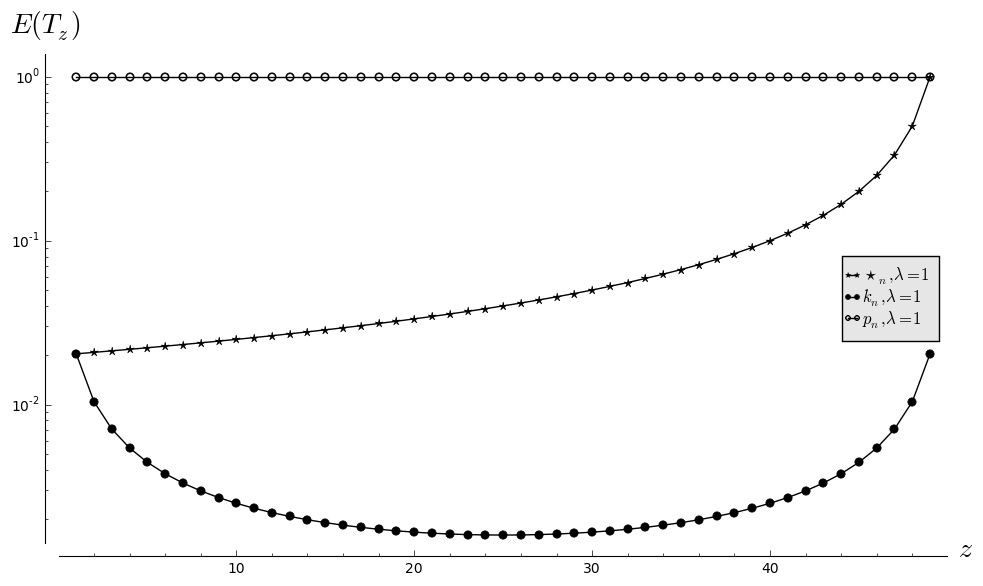
\includegraphics[scale=0.45]{figures/ETk.png}
\end{center}
\caption{Expected branch-lengths when there are $z$ infection events or $z+1$ infected individuals, $E(T_z)$, for the three cases. Here $n=50$ and $\lambda=1$. $E(T_z)=1/\lambda=1$ with the path network $p_n$ of \autoref{EX:TrPathNetwork}, $E(T_z)=1/(\lambda(n-z))=1/(50-z)$ with the star network $\star_n$ of \autoref{EX:TrStarNetwork} and $E(T_z)=1/(\lambda z(n-z))=1/(z(50-z))$ with the complete network $k_n$ of \autoref{EX:TrCompleteNetwork} as $z$ ranges in $\{1,2,\ldots,n-1=49\}$.\label{F:ETk}}
\end{center}
\end{figure}

\subsection{Branch-lengths}
We can obtain the expected branch-length of the transmission tree between the $(z-1)$-th and $z$-th infection event or equivalently when there are $z$ infected individuals by simply taking the mean of the exponentially distributed holding-time random variable in the generators given by \autorefs{E:GenCTchainProbkn}, \ref{E:GenCTchainProbsn} and \ref{E:GenCTchainProbpn} as shown in \autoref{F:ETk}.  
Here we take the $0$-th infection event as the initial infection.

\begin{figure}[htbp]
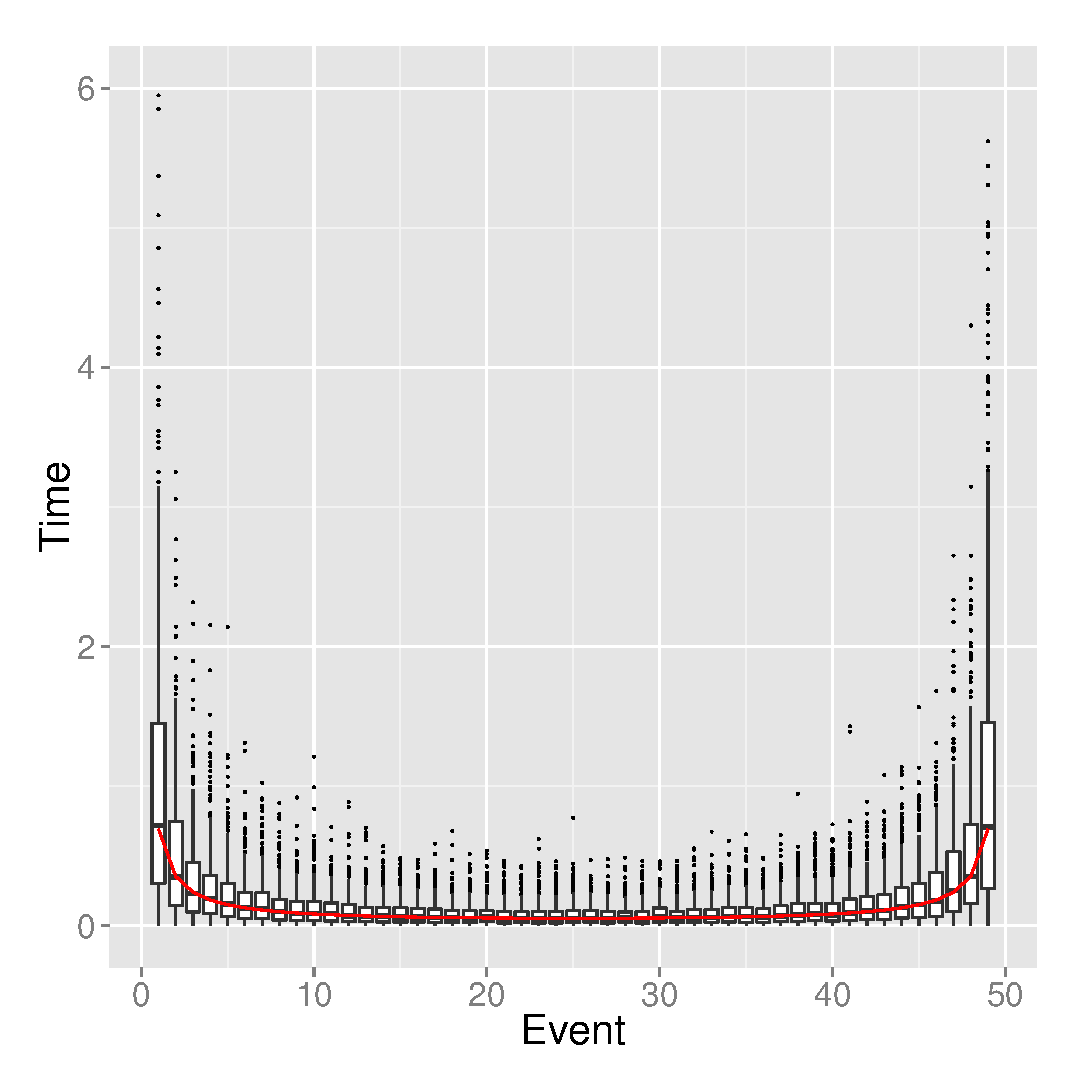
\includegraphics[width=0.95\linewidth]{figures/timesbox.eps}
\caption{The sampling distribution of $T_z$, branch-lengths (times in y-axis) of the transmission tree when there are exactly $z$ infected individuals or between the $(z-1)$-th and $z$-th infection event (x-axis), where $z \in \{1,2,\ldots,n-1\}$, from 500 independent simulations of the transmission tree over the complete SI contact network for a population of size $n=50$ (as box plots) and the median branch-lengths given by $E(T_z) \log 2=(\lambda z (n-z))^{-1}\log 2$, with $\lambda=1/(n-1)$ (as red solid line).\label{F:timesbox}}
\end{figure}

Thus, if the underlying SI contact network is $k_n$ then 
initially at the start of the transmission, the transition rate is $\lambda 1\times(n-1)$ 
with expected branch-length $E(T_1)=1/(\lambda (n-1))$, where $T_1$ is the duration of the epoch when there is only one infected individual.  
In general, $T_z$ is the duration of time when there are $z$ infected individuals and is the length of the transmission tree when there are $z$ branches, where $z \in [n-1]$.  
The transition rate $\lambda z \times (n-z)$ increases and the expected branch-length 
$E(T_z)=1/(\lambda z \times (n-z))$ decreases at the 
$z$-th infection event as $z$ increases to $n/2$.  
The expected branch-length is smallest at $4/(\lambda n^2)$ when $z=n/2$ and then starts increasing to $1/(\lambda (n-1))$ as $z \to n-1$ when all $n$ individuals are infected.  
This is shown as a ``bath-tub'' curve in \autoref{F:ETk}.  
This means that the branch length of the tree at the $z$-th transmission step, 
which gives the duration of continuous time taken for the $z$-th infection event, 
will have mean length $1/(\lambda z \times(n-z))$, 
such that any one of the $z$ infected leaf vertices can branch with uniform probability $1/z$ at equal rate $\lambda (n-z)$ to infect one of the $(n-z)$ susceptible (and yet uninfected) individuals with uniform probability $1/(n-z)$.  
The sampling distribution of branch-lengths between consecutive infection events from 500 independent simulations of the transmission tree is shown in \autoref{F:timesbox} and two typical transmission trees with branch-lengths and topologies over the complete SI contact network for a population of size $n=50$ is shown in \autoref{F:tree-rand12}.

Furthermore, by rescaling time in units of population size with $\lambda=1/(n-1)$, the 
time of the $z$-th infection event, $T_z$, is independent exponential random variable with rate $z(n-z)/(n-1)$ and satisfies the following {\em randomly-shifted-logistic-limit} (see for eg.~\cite[Eq. 7.13]{AldousIPSSSD2013}):
\[
T_{\lfloor un \rfloor} - \log n \overset{d}{\rightarrow} F^{-1}(u) + G, \quad 0<u<1,
\]
where, $F$ is the logistic function:
\[
F(t) = \frac{\exp(t)}{1+\exp(t)}, \quad -\infty < t < \infty
\]
and $G$ has Gumbel distribution with $\Pr(G<x)=\exp(e^{-x})$.

\begin{figure}[htbp]
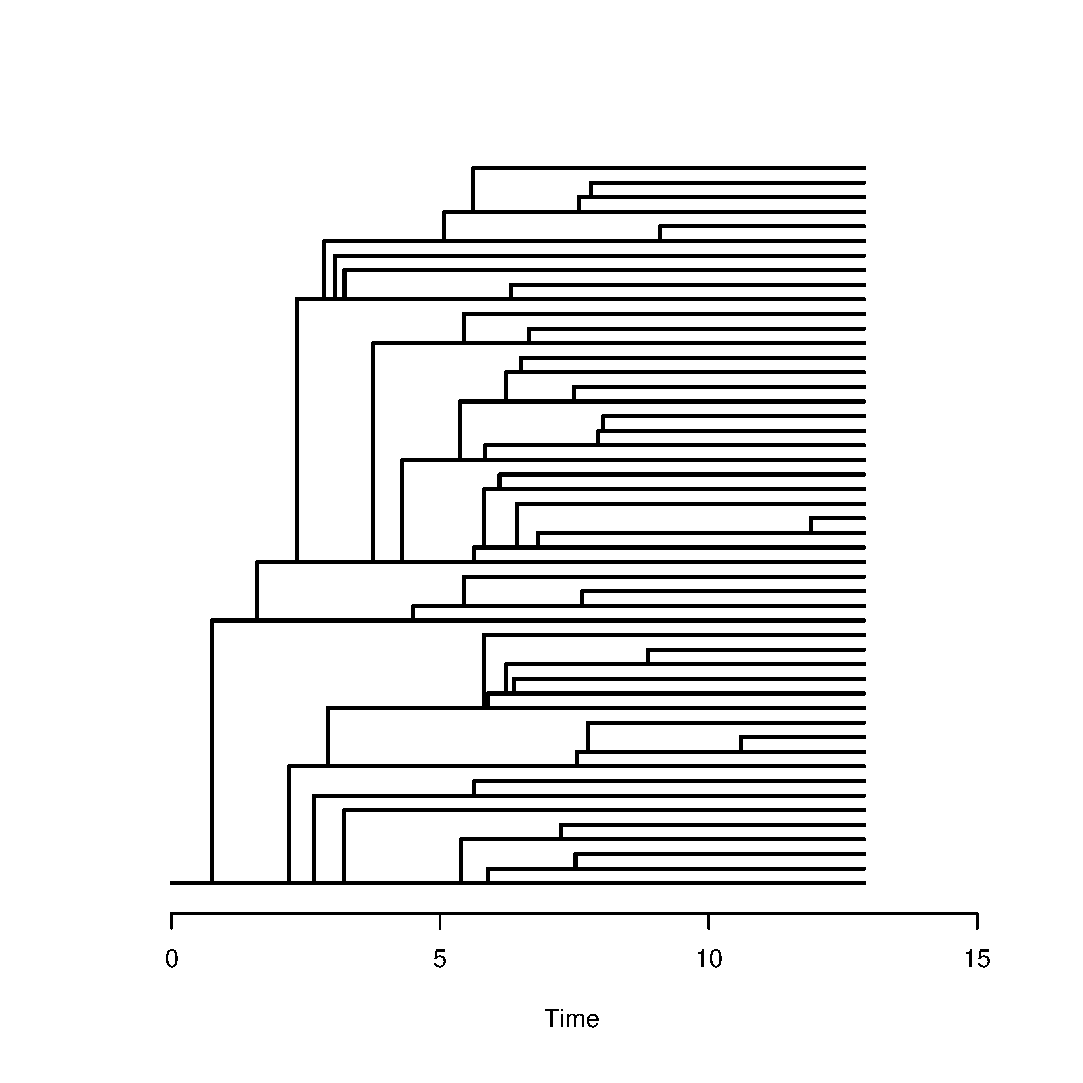
\includegraphics[width=0.5\linewidth]{figures/tree-rand1.eps}
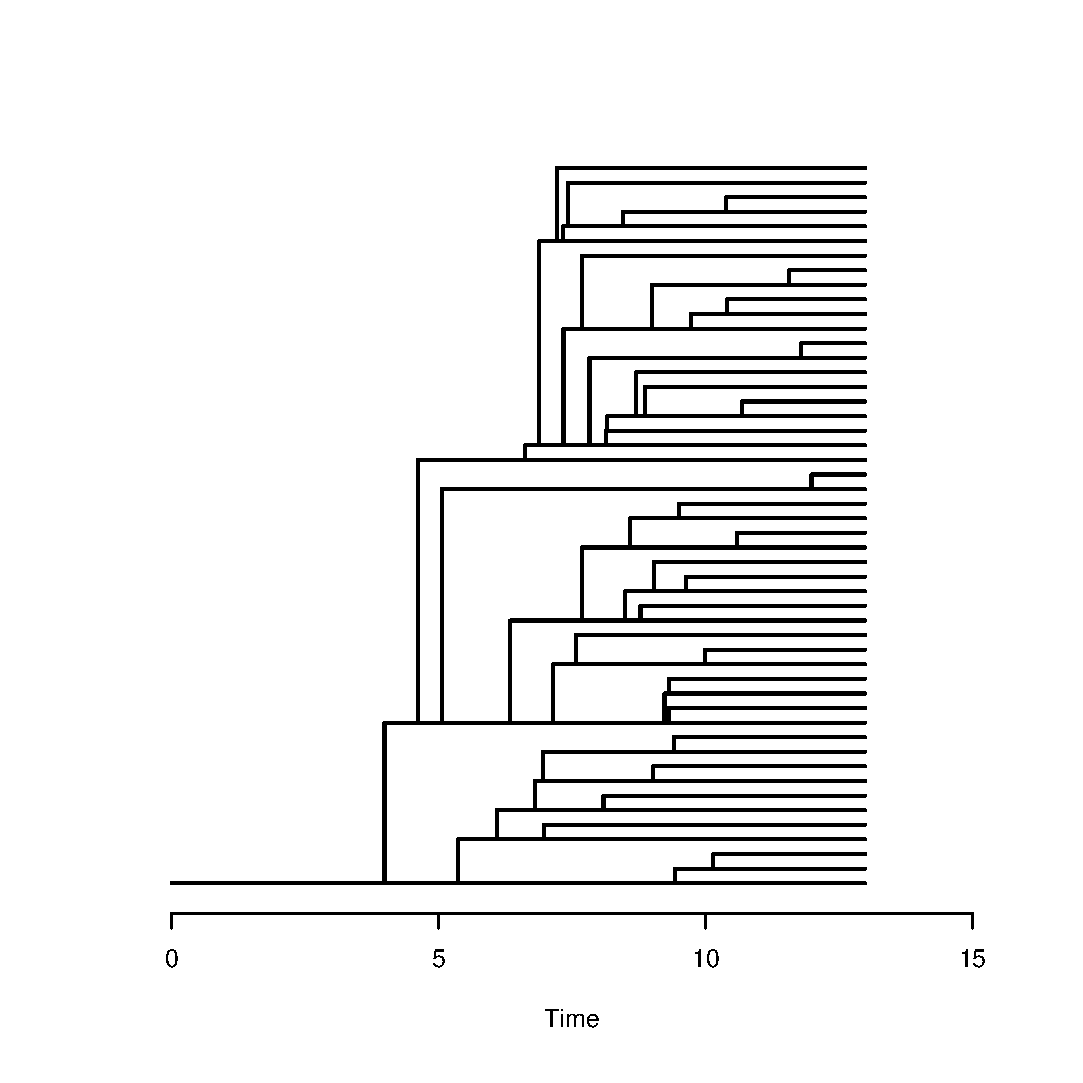
\includegraphics[width=0.5\linewidth]{figures/tree-rand2.eps}
\caption{Two of the 500 independent simulations of the (unlabelled) transmission tree with branch-lengths over the complete SI contact network for a population of size $50$ from \autoref{F:timesbox}. Notice the variation in branch-lengths (times between infection events) at the start and end of the epidemic when the variance is largest.\label{F:tree-rand12}}
\end{figure}


The expected branch-length $E(T_z)$, as a function of $z \in \{1,2,\ldots,n-1\}$, 
when the SI contact network is the star network ($\star_n$) or the path network ($p_n$), 
is inversely proportional to $(n-z)$ or independent of $z$ and $n$ with $E(T_z)$ 
equalling $1/(\lambda (n-z))$ or $1/\lambda$, respectively, as depicted in \autoref{F:ETk}. 


\section{A biparametric Beta-splitting transmission process}\label{S:BetaSplit}

We gave a non-parametric description of the transmission process for arbitrary contact networks in the previous section.  
This Markov construction over the state space of SI contact networks and transmission trees can be too detailed.  
Often, one does not have knowledge of the state space at this detailed resolution so it is useful to construct transmission processes without explicitly tracking the underlying SI contact network.  
Here, we give a parametric construction for such a process, by integrating over a Beta-splitting family of transmission trees with interval-labelled leaves, that captures the three Examples in \autorefs{EX:TrCompleteNetwork}, \ref{EX:TrStarNetwork} and \ref{EX:TrPathNetwork} as special cases.

The biparametric Beta-splitting model is described in \cite{SainudiinVeber2016} for evolutionary trees.  
We adapt that construction here for transmission trees.   
To match the standard definition of the Beta distribution, for any $\alpha,\beta>0$ we call $\calB(\alpha,\beta)$ the distribution on $[0,1]$ with density $B(\alpha,\beta)^{-1}x^{\alpha-1}(1-x)^{\beta-1}$, where
\begin{equation}\label{notation beta}
B(\alpha,\beta) := \int_0^1 x^{\alpha-1}(1-x)^{\beta-1}dx.
\end{equation}
If $\alpha=\beta$, this distribution is symmetric: if $X\sim \calB(\beta,\beta)$, then $1-X \sim \calB(\beta,\beta)$.  
We call $\calB(\alpha+1,\beta+1)$ as the Beta-splitting density (for $\alpha,\beta>-1$), with density proportional to $x^\alpha(1-x)^\beta$. 
This parametric choice corresponds to that used by \cite{Aldous2001} for the symmetric case with $\alpha=\beta$.


We fix $\alpha,\beta>-1$.  
Let $(B_1,B_2,\ldots)$ be a sequence of independent and identically distributed (i.i.d.) random variables, with the $\calB(\alpha+1,\beta+1)$ distribution.  
Let $(U_1,U_2,\ldots)$ be a sequence of i.i.d. random variables with the uniform distribution on $[0,1]$ that is independent of $(B_1,B_2,\ldots)$.  
Thus, each of these variables takes its values in $[0,1]$.  
We call $(G_z = (U_z,B_z))_{z\in \bN}$ the \emph{generating sequence} for the Beta-splitting trees.  
It will be the basis of an incremental construction of transmission tree as a labelled ranked planar binary tree with $m$ leaves and $m-1$ internal vertices.

Our core idea relies on decomposing the transmission tree construction into two stages: 
(1) constructing a random transmission tree without infector-infectee leaf labels such that 
it biparametrically captures an essential aspect of the underlying SI contact network's structure and 
(2) labelling the leaf vertices with infected individuals from $\bI_n$ for each transmission or splitting event from stage (1).  
Stage (2) is optional and the construction of transmission trees without leaf labels from $\bI_n$ can be obtained just from stage (1) --- such leaf-unlabelled transmission trees can still provide useful prior distributions for integration during inference with partial observations.

Stage (1) of the transmission tree construction involves a deterministic mapping followed by an integration.  
We first describe the deterministic mapping that takes a realization of the generating sequence $(G_z)_{z\in \bN}$ and turns it into a Beta-splitting tree, i.e.~a planar binary tree in which the internal vertices are ranked with integer labels and the leaves are labelled by subintervals that partition $[0,1]$. 
We then describe an integration over $(\alpha,\beta)$-specific random partitions by such sub-intervals.  

As we shall see below, the integer labels of the internal vertices will give the order in which these vertices have been split during the construction, i.e., the order of infections or successful transmissions.  
The interval labels of the leaves will form a partition of the interval $[0,1]$ and will be used to decide which leaf is split and becomes an internal vertex in the next step.  
The left and right leaf vertices resulting from a split stand for the infector and infectee in the underlying (unobserved) SI contact network after the infection event.

Let $(g_z=(u_z,b_z))_{z\in \bN}$ be a realization of the generating sequence. 
The {\em organizing map} $O(g)$ proceeds incrementally as follows, until the tree created has $m$ internal vertices and $m+1$ leaves.  
We start with a single root vertex, labelled by the interval $[0,1]$. 
\begin{itemize}
\item Step $1$: Split the root into a left leaf with interval label $[0,b_1]$ and a right leaf labelled by $[b_1,1]$.  Change the label of the root to the integer $1$.
\item Step $2$: If $u_2\in [0,b_1]$, split the left child vertex of the root into a left leaf and a right leaf labelled by $[0,b_1b_2]$ and $[b_1b_2,b_1]$, respectively.  If $u_2\in [b_1,1]$, then instead split the right child vertex of the root into left and right leaves with respective labels $[b_1,b_1+(1-b_1)b_2]$ and $[b_1+(1-b_1)b_2,1]$.  Label the former leaf that is split during this step by $2$.
\item Step $z$: Find the leaf whose label $[a,b]$ contains $u_z$.  
Change its label to the integer $z$ and split it into a left leaf with label $[a,a+(b-a)b_z]$ and a right leaf with label $[a+(b-a)b_z,b]$. 
\item Stop at the end of Step $m$.
\end{itemize}

In words, at each step $z$, the interval labels of the leaves form a partition of the interval $[0,1]$.  
We find the next leaf vertex to be split by checking which leaf interval contains the corresponding $u_z$ and then $b_z$ is used to split the interval of that former leaf, say with interval width $d$, into two intervals of lengths $b_z d$ and $(1-b_z)d$. 
Thus, the width of the left interval of a current leaf vertex that is about to be split should be constructed by the Beta-splitting density such that it is proportional to all infection events that will subtend from the current infector and its future infectees after this infection event.  
Similarly, the width of the right leaf label of this current leaf vertex should be such that it is proportional to all infection events that will subtend from the current infectee and its future infectees.  
Intuitively, one can think of the width of the interval label of a leaf vertex as the {\em infection potential} of the individual associated with that leaf and the widths of the left and right interval labels upon a split or an infection event as the infection potentials of the infector and the infectee, respectively, after the event.  
Thus, the Beta-splitting trees capture the essence of transmission trees that are co-evolving with underlying SI contact networks, without explicitly requiring complete knowledge of the networks during their construction.
The internal vertex just created is then labelled by $z$ to record the order of the splits.  
At the end of step $z$, the tree has $z+1$ leaves, and so we stop the procedure at step $m$ to ensure $m+1$ leaves, where $1 \leq m \leq n-1$.  
Figure~\ref{example1} shows an example of such a Beta-splitting tree construction for $m=3$. 


After the Beta-splitting construction, we first integrate over $(G_z)_{z\in \bN}$ to `erase' the interval-valued leaf labels and then assign infected individuals in $\bI_n$ as leaf labels to obtain transmission trees from integrated Beta-splitting trees. 
These trees have $m$ integer-labelled internal vertices or splits and $m+1$ unlabelled leaves.  
The process of assigning leaf labels from $\bI_n$ via a pre-order traversal on the $m$ internal vertices, in increasing order, i.e., Stage (2) of the construction, is described next.

We start with the internal vertex labelled $1$ and assign the initial infected individual $\imath_{i(0)}$ to its left child vertex. 
Then we assign the first infectee to the right child vertex of $1$.  
In general, as we descend down the internal vertices of the integrated Beta-splitting tree in increasing order of its integer labels we slide the individual label $\imath_{\ell}$ to the left 
of the split and assign a new label to the right vertex as the infectee $\imath_j$ chosen according to the infectee distribution for $\imath_{\ell}$: 
\begin{equation}\label{E:AssignInfectionLabels}
\imath_j \sim \{\Pr\{\imath_{\ell} \overset{z}{\rightsquigarrow} \imath_j \}:  \imath_j \in \bI_n \} \enspace,
\end{equation}
the probability that $\imath_{\ell}$ infects $\imath_j$ at discrete time-step $z$.
This distribution is defined to be generic on purpose, without necessarily making explicit reference to $c(z)$, 
the underlying SI contact network at time $z$, that is typically unknown or partially known.  
We can always obtain specific form for \autoref{E:AssignInfectionLabels} by making explicit assumptions on $c(z)$ via the infector-specific infectee distribution within \autoref{E:GenJumpchainProb}:
\begin{multline}\label{E:AssignInfectionLabelsExplicit}
\{\Pr\{\imath_{\ell} \overset{z+1}{\rightsquigarrow} \imath_j \}:  \imath_j \in \bI_n \}
=
\begin{cases}
\frac{w(\imath_{\ell},\imath_j;\, c(z))}
{\sum\limits_{\substack{\forall \imath_j \in \bI_n :\\ s_j(z)=1}}
w(\imath_{\ell},\imath_j ; c(z))}
& \text{ if } (\tau(z),c(z)) \prec (\tau(z+1),c(z+1))\\
0 & \text{ otherwise}.
\end{cases}
\end{multline}


\begin{figure}[t]
\begin{center}
%\input{figures/figure1.pdf_t}
\input{figures/figure1.latex}
\caption{\label{example1}An example of a Beta-splitting tree construction for $m=3$.}
\end{center}
\end{figure}


\subsection{Probability of a given Beta-splitting transmission tree}

For a given (leaf-unlabelled) ranked planar tree, and an internal vertex labelled by $i$, let us write $s_i^L$ (resp., $s_i^R$) for the number of internal vertices in the left (resp., right) subtree below vertex $i$. In particular, if vertex $i$ subtends two leaves, then $s_i^L=0=s_i^R$.

\smallskip
\begin{theorem}\label{th:proba}
The probability of any discrete transmission tree $\tau(m)$ with $m$ splits and $m+1$ leaves under the integrated Beta-splitting model is:
\begin{align}
\Pr\{\tau(m)\} &= \prod_{z=1}^{m} \left\{\frac{1}{B(\alpha+1,\beta+1)}\int_0^1 b_z^{s_z^L+\alpha}(1-b_z)^{s_z^R+\beta}db_z\right\}  \times \Pr\left( \textrm{leaf labels} \right)\nonumber\\
& = \prod_{z=1}^{m} \frac{B(s_z^L+\alpha+1,s_z^R+\beta+1)}{B(\alpha+1,\beta+1)} \times \Pr\left( \textrm{leaf labels} \right) , \label{proba}\\
& = \prod_{z=1}^{m} \left( \frac{\prod_{j=0}^{s_z^R}\frac{\beta+j}{\beta+j+\alpha} \prod_{i=0}^{s_z^L} \frac{\alpha+i}{\alpha+i+\beta+s_z^R+1}}
{\frac{\alpha \beta}{(\alpha+\beta)(\alpha+\beta+1)}}\right) \times \Pr\left( \textrm{leaf labels} \right), \label{prob2a}
%\prod_{(s^L,s^R) \in \mathcal{S}_n} \left(\frac{\prod_{j=0}^{s^R}\frac{\beta+j}{\beta+j+\alpha} \prod_{i=0}^{s^L} \frac{\alpha+i}{\alpha+i+\beta+s^R+1}}
%{\frac{\alpha \beta}{(\alpha+\beta)(\alpha+\beta+1)}}\right)^{f(s^L,s^R)}.
\end{align}
where $B(\alpha,\beta)$ was defined in \autoref{notation beta} and 
\begin{equation}\label{E:ProbOfTTLeafLabels}
\Pr\left( \textrm{leaf labels} \right) = \Pr\{\imath_{i(0)}\} \prod_{z=1}^m \Pr\{(L(z);\tau(z)) \overset{z-1}{\rightsquigarrow} (R(z);\tau(z))\} \enspace.
\end{equation}
\end{theorem}

\smallskip
\noindent\textbf{Proof outline.} 
The second term in the product of \autoref{proba} and \autoref{prob2a} given by \autoref{E:ProbOfTTLeafLabels} is due to the independent assignment of infected individual according to \autoref{E:AssignInfectionLabels} as we recursively descend through the infection events encoded by the ranked internal vertices of the tree after the initial infection with $\Pr\{\imath_{i(0)}\}$. 

We now focus on the first term in \autoref{proba} which results from integrating over the $(U_z,B_z)_{z\in[m]}$, for $1\leq m \leq n-1$.  
Remember that if a leaf is labelled by an interval $[a,b]$, the probability that it is split during the $z$-th step is $b-a$, the probability that the uniform random variable $U_z$ falls within $[a,b]\subset[0,1]$.  
If it is chosen to split, it is given label $z$ and the left and right leaves created are labelled by intervals of respective lengths $B_z(b-a)$ and $(1-B_z)(b-a)$.  
Then these intervals may split later, but into intervals of lengths that are always proportional to $B_z$ or $1-B_z$ (respectively).  
Now the probability of the tree $\tau$ is the product of the $m$ probabilities of choosing a given leaf to split at each step, each of which is equal to the length of the interval labeling that leaf.  
As a consequence, each split occurring in the left subtree below vertex $z$ brings in another $B_z$ in the product, or another $1-B_z$ if the split occurs in the right subtree below vertex $z$.  
Averaging over the possible values of the $B_z$'s, which are independent $\mathcal{B}(\alpha+1,\beta+1)$ random variables, yields the result. 

Finally, to prove the first term in \autoref{prob2a} we exploit the fact that $s^L$ and $s^R$ are non-negative integers and repeatedly apply the following elementary properties of the beta function: 
\begin{equation}\label{E:integerPropBetaFunc}
B(x+1,y)=B(x,y)\frac{x}{x+y}, \quad B(x,y+1)=B(x,y)\frac{y}{x+y} \enspace.
\end{equation}
\hfill $\Box$

\begin{remark}
Note that the expression for the probability of a transmission tree with $m$ infection events given by \autoref{prob2a} as a function of the parameters $\alpha$ and $\beta$, i.e., the likelihood function, only involves additions, multiplications and divisions.  
It is therefore numerically more robust during local optimization for maximum likelihood estimation in \autoref{S:MLE} than the expression in \autoref{proba}, which further requires numerical evaluations of the beta function. 
\end{remark}

\subsection{Examples}\label{S:Examples-betaSplitting}

Now we reconsider the three specific SI contact networks and show that they arise for specific values of $\alpha$ and $\beta$.  

Recall that $B(\alpha,\beta)$ is related to the Gamma function $\Gamma$ by the equality
\begin{equation}
B(\alpha,\beta)=\frac{\Gamma(\alpha)\Gamma(\beta)}{\Gamma(\alpha+\beta)},\qquad \alpha,\beta>0,
\end{equation}
and that $\Gamma(\beta)=(\beta-1)!=(\beta-1)(\beta-2)\cdots 2\cdot 1$ if $\beta\in \bN$. 

\subsubsection{Complete network underlies Beta-splitting transmission trees with $\alpha=\beta=0$}
Let us assume that the initial infection is uniformly distributed in $\bI_n$ and that the SICN is the complete contact network $k_n$ with unit weights as in \autoref{EX:TrCompleteNetwork} and show that the probability of the discrete transmission tree after $m$ infections has the same probability as \autoref{E:GenCTchainProbknTree}.  

The first term in \autoref{proba} with $\alpha=\beta = 0$, simplifies as follows:
\begin{equation}\label{E:beta0}
\prod_{z=1}^{m} \frac{B(s_z^L+1,s_z^R+1)}{B(1,1)}= \prod_{z=1}^{m} \frac{s_z^L!s_z^R!}{(s_z^L+s_z^R+1)!} = \frac{1}{m!},
\end{equation}
where the second equality is obtained by observing that $s_z^L+s_z^R+1$ is the number of internal vertices of the tree rooted at vertex $z$, which is the left or the right subtree below the internal vertex $z$.  
Hence, each term $s_z^L!$ in the numerator of the product cancels with the term in the denominator that corresponds to the left child vertex of $z$, except if $s_z^L=0$ and the left child vertex of $z$ is a leaf.  
But in this case, $0!=1$ by convention.  
The same holds true for each of the $s_z^R!$.  
Likewise, the terms in the denominator which are not compensated by some term in the numerator are those corresponding to internal vertices having no ancestral vertices.  
But the only such vertex is the root ($z=1$) with $s_1^L+s_1^R+1=m$.  
This gives us the result.

From \autoref{E:AssignInfectionLabelsExplicit}, the infectee probability is uniformly distributed over $n-z$ infectees for each infector at time-step $z$ and thus the second term in \autoref{proba} simplifies to:
\begin{equation}\label{E:knAB02ndTerm}
\Pr\{\imath_{i(0)}\} \prod_{z=1}^m \Pr\{(L(z);\tau(z)) \overset{z-1}{\rightsquigarrow} (R(z);\tau(z))\} = \frac{1}{n} \prod_{z=1}^m \frac{1}{n-z} = \frac{(n-m-1)!}{n!}
\end{equation}
Finally, putting \Autorefs{E:beta0} and \ref{E:knAB02ndTerm} into \autoref{proba}, we get the desired identity with \autoref{E:GenCTchainProbknTree}.  
Since the probabilities of the discrete transmission trees are identical between the integrated Beta-splitting trees with $\alpha=\beta=0$ and the construction of \autoref{EX:TrCompleteNetwork} with an explicit complete SI contact network, the continuous-time process will also be identical to \autoref{E:GenCTchainProbkn} due to independent Exponential rates for the infection events.

\begin{remark}
The transmission tree thus constructed with $\alpha=\beta=0$ corresponds to \cite{Yule1924} model for evolutionary trees (ignoring planarity and leaf labels).  
This Beta-splitting construction is very different from the standard evolutionary construction of the Yule tree, in which the next leaf to split is chosen uniformly at random from among the current set of leaves.  
Here the choice of the next split is dictated by the lengths of the intervals labeling the current leaves, which will all be distinct will probability one.  
However, by averaging over the law of the generating sequence (when $\alpha=\beta=0$) yields the same uniform distribution on rooted ranked planar binary trees with $m$ splits and $m+1$ unlabelled leaves.
These $m!$ many trees are in bijective correspondence with permutations of $\{1,\ldots,m\}$ through the {\em increasing binary tree-lifting} operation \cite[Ex 17, p.~132]{Flajolet}.
\end{remark}


\subsubsection{Star network underlies Beta-splitting transmission trees with $\alpha \to \infty, \beta \to -1$}\label{S:StarBeta}

To obtain a left-branching comb we let $(\alpha,\beta)$ approach the limiting bottom-right corner $(\infty,-1)$ of the parameter space.  
As $\alpha \to \infty$ from the left and $\beta\rightarrow -1$ from above, the $\calB(\alpha+1,\beta+1)$ distribution concentrates on the boundary of the support at $1$.  
In the limit, each random variable $B_z$ in the generating sequence takes the value $1$, with probability $1$.  
Thus, the root is first split into a left leaf with label $[0,1]$ and a right leaf with label $\{1\}$ (i.e., an interval reduced to a single point $1$).  
Next, the uniform random variable $U_2$ belongs to the interval $[0,1]$ with probability one, so that the left leaf labelled by $[0,1]$ is necessarily that chosen to split next.  
Again, it is split into two leaves with left leaf label $[0,1]$ and right leaf label $\{1\}$, implying that the next leaf to split is again the left one which inherited the full interval $[0,1]$ with probability one.  
This recursive reasoning can be carried on until step $m$ with $m+1$ leaves.  
Hence, morally the tree corresponding to $\alpha \to \infty$ and $\beta \to -1$ is a fully unbalanced tree, with a left-branching comb with $m+1$ leaves.  
See \autoref{F:starpath4} for an example with $m=3$.
Recall that this is exactly the transmission tree obtained when the underlying SICN is the star network of \autoref{EX:TrStarNetwork}.

For Stage (2) of the construction where we assign leaf labels to the integrated Beta-splitting tree we assume that the underlying SICN is the star network initialized at the source vertex.  
Since there is only one discrete transmission tree topology, i.e., the left-branching comb, 
we can label the leaves of the integrated Beta-splitting tree in $\prod_{z=1}^{m} \left( \frac{1}{n-z}\right)$ many ways to obtain the same probability in \autoref{E:GenCTchainProbrsnTree} for the discrete transmission tree with individuals leaf labels from $\bI_n$. 

\begin{figure}[t]
\begin {center}
\scalebox{.85}{
\input{figures/starpath4.latex}
}
\end{center}
\caption{\label{F:starpath4}(a) The discrete transmission tree corresponding to the limiting case $\alpha \to \infty$ and $\beta \to -1$ is a left-branching comb, and (b) the discrete transmission tree corresponding to the limiting case $\beta \to \infty$ and $\alpha \to -1$ is a right-branching comb.}
\end{figure}


\subsubsection{Path network underlies Beta-splitting transmission trees with $\alpha \to -1, \beta \to \infty$}\label{S:PathNetworkbetaSplitting}

By an analogous argument to that in \autoref{S:StarBeta} with $\beta \to \infty$ and $\alpha \to -1$, the $\calB(\alpha+1,\beta+1)$ distribution concentrates on the boundary of the support at $0$ and each random variable $B_z$ in the generating sequence takes the value $0$, with probability $1$.  
Thus, the only discrete transmission tree topology for the Beta-splitting tree with $(\alpha,\beta) \to (-1,\infty)$, the limiting top-left corner of the parameter space, is the right-branching comb shown in \autoref{F:starpath4} (b), the same one obtained by assuming that the underlying SICN is the path network in \autoref{EX:TrPathNetwork}.  
By further assuming that the underlying SICN is the path network for the leaf-labelling Stage (2) with the initial infection spreading from the individual $\imath_{\hookrightarrow}$ at the beginning of the path as in \autoref{EX:TrPathNetwork}, we obtain exactly one possible labelling and obtain the same probability in \autoref{E:GenCTchainProbrpnTree}. 


\subsection{Maximum likelihood estimation and sufficient statistics}\label{S:MLE}

In order to find the maximum likelihood estimates of $\alpha$ and $\beta$ for the Beta-splitting model that give the most likely explanation for the transmission trees sampled from an arbitrary SICN (under the likelihood principle), we use the following inferential procedure:
\begin{enumerate} 
\item[Step~1:]{Generate a sample of $r$ independent transmission trees $(\tau_1,\tau_2,\ldots,\tau_r)$ from:
\begin{itemize}
\item the given SICN {\tt C} and 
\item initial infected individual {\tt initialI} 
\end{itemize}
by calling {\tt transmissionProcessTC(C,initialI)} in \autoref{Sec:codeA} $r$ times.}
\item[Step~2:]{Compute $(\widehat{\alpha},\widehat{\beta})$, the maximum likelihood estimate (MLE) of the parameters by maximizing the likelihood function as follows:}
\end{enumerate}
\[
(\widehat{\alpha},\widehat{\beta}) = \argmax_{(\alpha,\beta) \in (-1,\infty) \times (-1,\infty)} \quad \prod_{i=1}^r \Pr(\tau_i; \alpha, \beta) \enspace.
\]
The probability of the tree $\tau_i$ for a given $(\alpha, \beta)$, $\Pr(\tau_i; \alpha, \beta)$, is obtained from a post-order traversal of $\tau_i$ to compute the first term in \autoref{proba}.  
To focus on the jump chain's discrete structural information in the transmission trees, our likelihood of the transmission tree ignores leaf labels and the waiting times between events as implemented in \autoref{Sec:codeC}.  
Note that such additional information can be easily incorporated into more elaborate likelihood functions derived from \autoref{E:GenCTchainProb} as outlined in \autorefs{R:ElaborateLklFuncs1} and \ref{R:ElaborateLklFuncs2}.  

\begin{theorem}\label{th:suff}
The likelihood of all $r$ transmission tree topologies only depends on the sufficient statistic of {\em split-pair frequencies}: 
\begin{multline}\label{E:SuffStats}
\{f(s^L,s^R): (s^L,s^R) \in \mathcal{S}_n \}, \quad \\ \text{where }, \mathcal{S}_n := \{(s^L,s^R) \in \{0,1,\ldots,n-2\}^2 : s^L+s^R \leq n-2\} \enspace.
\end{multline}
Therefore, the maximum likelihood point estimate for the Beta-splitting model based on $r$ independent transmission trees, each with $n$ leaves, is obtained by maximizing the per-vertex loglikelihood:
\begin{equation}\label{E:perNodeMLE}
(\widehat{\alpha},\widehat{\beta}) = \argmax_{(\alpha,\beta) \in (-1,\infty)^2} \quad 
\sum_{(s^L,s^R) \in \mathcal{S}_n} {\hat{P}(s^L,s^R)} \, \log\left(\frac{\prod_{j=0}^{s^R}\frac{\beta+j}{\beta+j+\alpha} \prod_{i=0}^{s^L} \frac{\alpha+i}{\alpha+i+\beta+s^R+1}}
{\frac{\alpha \beta}{(\alpha+\beta)(\alpha+\beta+1)}}\right) \enspace,
\end{equation}
where, $\hat{P}(s^L,s^R):=f(s^L,s^R)/(n-1)r$ and 
$f(s^L,s^R)$ is the frequency of the $(n-1)r$ many internal vertices across all $r$ trees that have $s^L$ and $s^R$ many splits in their left and right sub-trees, provided $n>1$.
\end{theorem}

\smallskip
\noindent\textbf{Proof.} 
From \autoref{proba} in \autoref{th:proba} and the assumption of independence across all $r$ trees:
\begin{align}
\prod_{i=1}^r \Pr(\tau_i; \alpha, \beta)  
&= \quad \prod_{i=1}^r \quad \prod_{z \in \mathcal{I}(\tau_i)}\frac{B(s_z^L+\alpha+1,s_z^R+\beta+1)}{B(\alpha+1,\beta+1)} \label{E:lkl0}\\
&= \prod_{(s^L,s^R) \in \mathcal{S}_n} \left( \frac{B(s^L+\alpha+1,s^R+\beta+1)}{B(\alpha+1,\beta+1)} \right)^{f(s^L,s^R)}\enspace. \label{E:lkl1}
\end{align}
Using the fact that $s^L$ and $s^R$ are non-negative integers we can exploit the properties of the beta function given by \autoref{E:integerPropBetaFunc} to further simplify the likelihood function from Equation~\ref{E:lkl1}, as follows:
\begin{align}\label{E:lkl2}
\prod_{i=1}^r \Pr(\tau_i; \alpha, \beta) 
&=
\prod_{(s^L,s^R) \in \mathcal{S}_n} \left(\frac{\prod_{j=0}^{s^R}\frac{\beta+j}{\beta+j+\alpha} \prod_{i=0}^{s^L} \frac{\alpha+i}{\alpha+i+\beta+s^R+1}}
{\frac{\alpha \beta}{(\alpha+\beta)(\alpha+\beta+1)}}\right)^{f(s^L,s^R)}.
\end{align}
Thus, the likelihood function only depends on the transmission trees up to the {\em split-pair frequencies} as claimed above \autoref{E:SuffStats} in the Theorem.

Next we derive the maximum likelihood estimate (MLE) in \autoref{E:perNodeMLE}.  
The MLE $(\widehat{\alpha},\widehat{\beta})$ obtained by maximizing the logarithm of the likelihood function in \autoref{E:lkl2}, for the purposes of point estimation, is equivalent to maximizing the per-vertex loglikelihood by ignoring the constant $(n-1)r$ as follows:
\begin{multline*} 
%(\widehat{\alpha},\widehat{\beta}) 
\argmax_{(\alpha,\beta) \in (-1,\infty)^2} \, 
(n-1)r \sum_{(s^L,s^R) \in \mathcal{S}_n} \frac{f(s^L,s^R)}{(n-1)r} \, \log\left(\frac{\prod_{j=0}^{s^R}\frac{\beta+j}{\beta+j+\alpha} \prod_{i=0}^{s^L} \frac{\alpha+i}{\alpha+i+\beta+s^R+1}}
{\frac{\alpha \beta}{(\alpha+\beta)(\alpha+\beta+1)}}\right) \\
= \argmax_{(\alpha,\beta) \in (-1,\infty)^2} \, 
\sum_{(s^L,s^R) \in \mathcal{S}_n} {\hat{P}(s^L,s^R)} \, \log\left(\frac{\prod_{j=0}^{s^R}\frac{\beta+j}{\beta+j+\alpha} \prod_{i=0}^{s^L} \frac{\alpha+i}{\alpha+i+\beta+s^R+1}}
{\frac{\alpha \beta}{(\alpha+\beta)(\alpha+\beta+1)}}\right) \enspace.
\end{multline*}
\hfill $\Box$

To focus on the jump chain's discrete structural information about the combinatorial skeletons of the contact network buried within the distribution over discrete transmission trees, as a necessary prelude to \autoref{T:effectiveBetaSplitting}, 
our likelihood expressions in \autorefs{E:perNodeMLE}, \ref{E:lkl0},\ref{E:lkl1} and \ref{E:lkl2} are {\em skeletal} and ignore leaf labels and the waiting times between events (see code in \autoref{Sec:codeC}).  
However, the likelihood function can be extended as discussed in \autoref{S:NaturalExtensionsOfTheLikelihoodFunction}.

The demonstration at the end of \autoref{Sec:codeC} shows two independent MLE computations based on $r=10$ independent transmission trees (without branch-lengths and leaf labels) that were sampled from the complete SICN on $n=50$ vertices.  
The MLE $(\widehat{\alpha},\widehat{\beta})$ takes the following realizations: 
$(-0.0664, -0.0502)$ and $(0.0047, -0.0430)$.  
As expected, these are close to $(\alpha,\beta)=(0,0)$, the parameters of the Beta-splitting model corresponding to the transmission tree distribution generated from the complete SICN.  
The variability in MLE is expected due to natural sampling variability.  
The MLE is $(0.0279, 0.0325)$ from another trial based on $r=1000$ independent transmission trees drawn from the same complete SICN on $50$ vertices.  
Figure~\ref{F:SuffStatsCompleteGraph_n50_reps10} shows the sufficient statistics for the parameters $\alpha$ and $\beta$ in these three trials.

\begin{figure}[htbp]
\begin{center}
\begin {center}
\scalebox{0.95}{
(a)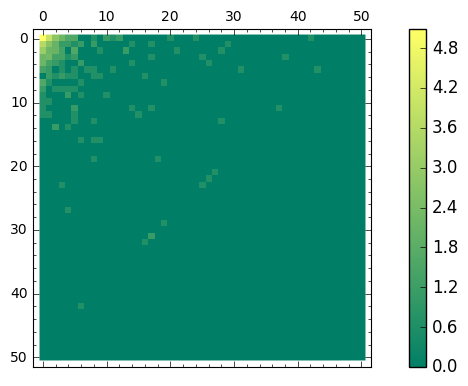
\includegraphics[width=0.29\linewidth]{figures/SuffStatsCompleteGraph_n50_reps10_mp1.png}\quad
(b)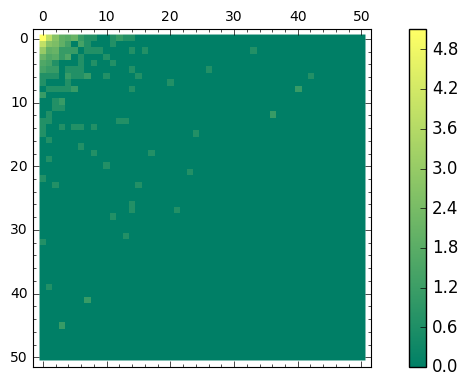
\includegraphics[width=0.29\linewidth]{figures/SuffStatsCompleteGraph_n50_reps10_mp2.png}\quad
(c)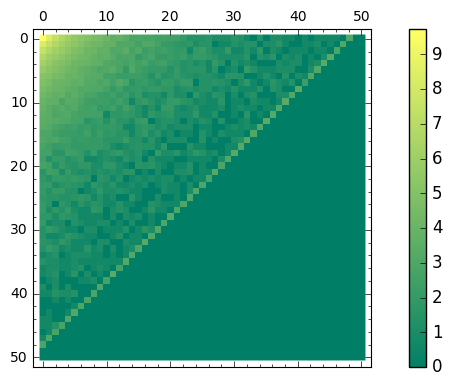
\includegraphics[width=0.29\linewidth]{figures/SuffStatsCompleteGraph_n50_reps1000_mp3.png}
}
\end{center}
\caption{Sufficient statistic of split-pair frequencies $f(s^L,s^R)$ on $\mathcal{S}_{50}$ from transmission trees on the complete network over $50$ vertices. 
Subplots (a) and (b) are for the two trials involving ten independent trees and subplot (c) is for a trial involving $1000$ independent trees.  
The frequencies are displayed as $\log(1+f(s^L,s^R))$.\label{F:SuffStatsCompleteGraph_n50_reps10}}
\end{center}
\end{figure}

\subsection{Equivalence class of contact networks with the same Beta-splitting model}\label{S:EquivClass}

The maximum likelihood estimate and the sufficient statistics for the parameters from \autoref{S:MLE} finally lead to a partitioning of all contact networks by an equivalence relation of having the same {\em effective Beta-splitting model for transmission trees}. 
Consider $\mathcal{C}_n^0$, the set of all initial SICNs, i.e., the set of all SI-tagged contact networks on $n$ vertices with a single initial infector labelled without loss of generality by $\imath_0$ and from whom the infection can spread to the remaining $n-1$ individuals: $\imath_0,\imath_1,\ldots,\imath_{n-1}$.  
Thus, $\mathcal{C}_n^0$ is the set of all initial distributions starting from a single individual for our Markov chain in \ref{E:GenJumpchainProbpn}, 
i.e. with initial condition $(\tau(0),c(0))$, where $\tau(0)$ is the tree with $\imath_0$ as its only vertex and $c(0)$ is the initial SICN.  
Note that $c(0)$, being an SICN, encodes that $\imath_0$ is infected and all other vertices are uninfected initially.
Let $\Pr(\tau; c(0))$ be the probability distribution on the space of transmission trees with $n$ leaves (without branch-lengths) at the end of the transmission process (when all $n$ individuals are infected) after starting from $c(0)$ according to \ref{E:GenJumpchainProbpn}.  
Finally let $\{\Pr((s^L,s^R); c(0)) : (s^L,s^R) \in \mathcal{S}_n\}$ be the probability distribution on the split-pairs in $\mathcal{S}_n$ that is further induced by $\Pr(\tau; c(0))$.  
Note that as the number of independent transmission trees $r$ approaches infinity, 
the empirical relative frequency $\hat{P}((s^L,s^R); c(0)):=f(s^L,s^R)/(n-1)r$ that is 
obtained from $r$ trees sampled from $\Pr(\tau; c(0))$, 
will converge with probability $1$ by Borel's law of large numbers to the probabilities for each split-pair $(s^L,s^R)$ in $\mathcal{S}_n$, 
as follows:
\[
\lim_{r\to\infty} \hat{P}((s^L,s^R); c(0)) = \Pr((s^L,s^R); c(0)) , \ \text{ for each } (s^L,s^R) \in \mathcal{S}_n \enspace.
\]
Thus, the use of $\Pr((s^L,s^R); c(0))$ instead of $\hat{P}((s^L,s^R); c(0))$ in the per-vertex loglikelihood of \autoref{E:perNodeMLE} will produce an asymptotic or exact and possibly set-valued MLE in a deterministic manner without any standard error that is caused by finite $r$.  
We use this fact to prove \autoref{T:effectiveBetaSplitting}.

\begin{theorem}\label{T:effectiveBetaSplitting}
Let the equivalence relation on $\mathcal{C}_n^0$ given by: 
\begin{equation}\label{E:Thm3E1}
c(0) \sim c'(0) \iff \left(\Pr((s^L,s^R); c(0))=\Pr((s^L,s^R); c'(0)) \ \text{ for each } (s^L,s^R) \in \mathcal{S}_n \right) \enspace,
\end{equation}
define the equivalence class $[c(0)]:= \{c'(0) : c(0) \sim c'(0)\}$, such that 
the set of equivalence classes $\mathfrak{C}_n^0 := \{ [c(0)] \}$ form a partition of $\mathcal{C}_n^0$ up to being identified by each distribution in  
\begin{equation}\label{E:Thm3E2}
\mathfrak{S}_n^0 := \left\{ \left\{\Pr((s^L,s^R); [c(0)]) : (s^L,s^R) \in \mathcal{S}_n \right\} : [c(0)] \in \mathfrak{C}_n^0 \right\} \enspace,
\end{equation} 
the set of all distributions over the split-pairs in $\mathcal{S}_n$ that is generated by the transmission process unfolding on the product space of transmission trees and SICNs with any initial SICN in each $[c(0)]\in \mathfrak{C}_n^0$.

Then for each equivalence class $[c(0)]$ we can obtain its effective Beta-splitting model with 
parameters $(\alpha^*,\beta^*)$ given by the exact MLE involving $\Pr((s^L,s^R); [c(0)])$ over each $(s^L,s^R) \in \mathcal{S}_n$ as specified by \autoref{E:ExactMLE}.
In other words, if two initial SICNs in $\mathcal{C}_n^0$ have the same distribution of split-pairs on $\mathcal{S}_n$ then they are indistinguishable by the exact MLE of the Beta-splitting model.  
We refer to the following map as the {\em Beta-projection} of the initial SICNs into the quarter-plane:
\begin{equation}\label{E:Thm3E3}
\mathcal{B}^{\downarrow}(c(0)) = (\alpha^*,\beta^*): \mathcal{C}_n^0 \to (-1,\infty)^2\enspace,
\end{equation}
and denote its inverse image by $\mathcal{B}^{\uparrow}(\alpha^*,\beta^*) : (-1,\infty)^2 \to \mathfrak{C}_n^0$.
\end{theorem}

\smallskip
\noindent\textbf{Proof outline.} 
The first part of the theorem is merely defining the equivalence class.
The proof is a direct consequence of all initial SICNs in $[c(0)]$ being indistinguishable 
by the asymptotic maximum likelihood estimator 
that is confined to the information in $\{\Pr((s^L,s^R);[c(0)])\}$  
under the Beta-splitting model: 
\begin{equation}\label{E:ExactMLE}
(\alpha^*,\beta^*) := \argmax_{(\alpha,\beta) \in (-1,\infty)^2} \, 
\prod_{(s^L,s^R) \in \mathcal{S}_n} \left(\frac{\prod_{j=0}^{s^R}\frac{\beta+j}{\beta+j+\alpha} \prod_{i=0}^{s^L} \frac{\alpha+i}{\alpha+i+\beta+s^R+1}}
{\frac{\alpha \beta}{(\alpha+\beta)(\alpha+\beta+1)}}\right)^{\Pr((s^L,s^R);[c(0)])} \enspace.
\end{equation}
We simply define the map and its inverse image in \autoref{E:Thm3E3}.
\hfill $\Box$

Note that this equivalence relation is based on the rooted ranked planar binary topology of the tree and ignores other informative statistics of the transmission tree, including waiting times and individual labels.  

\begin{remark}\label{R:practicalMLE}
In practise, we will only be able to obtain the estimated effective Beta-splitting model associated with an initial SICN by finding $(\widehat{\alpha},\widehat{\beta})$, the MLE from finitely many transmission trees drawn from the transmission process (i.e., with $r < \infty$ and positive standard error).  
As shown in \autoref{T:mles} and \autoref{F:tableIDMLEStdErrZoomed}, the MLEs can distinguish different underlying contact networks even when $r$ is finite.  
\end{remark}

\subsubsection{Elements from the equivalence class of the source-initialized path network}\label{S:UnidirectionalCircularNetwork}
To show that this equivalence relation is non-trivial, we give a concrete example of an equivalence class that not only contains the path network initialized at the source vertex (as in \autoref{S:PathNetworkbetaSplitting}) but also $n$ other initial SICNs.
Recall that the only discrete transmission tree topology for the Beta-splitting tree with $(\alpha,\beta) \to (-1,\infty)$, 
is the right-branching comb, the same one obtained by assuming that the underlying SICN is the path network 
with the initial infection spreading from the individual, say $\imath_{0}$, at the beginning of the path or the source vertex as in \autoref{EX:TrPathNetwork}.   
To obtain other initial SICNs in the same equivalence class as the path network that is initially infected at the source vertex, let us consider the {\em unidirectional circular network} on $n$ vertices given by $\{\imath_0,\imath_1,\ldots,\imath_{n-1}\}$ and $n$ directed edges given by $\{(\imath_0,\imath_1), (\imath_1,\imath_2), \ldots, (\imath_{n-2},\imath_{n-1}), (\imath_{n-1},\imath_0)\}$.  We can imagine the network being laid out on the plane along a circle.    
It is clear that we can have the infection initialized from any $\imath_i$ and it will spread sequentially along the circular path until all remaining individuals are infected in tandem, say anti-clockwise.
Thus the transmission tree (ignoring leaf labels) generated on the unidirectional circular network by starting from any one of the $n$ individuals is identical to the right-branching comb under the path network initialized at the source vertex. 
This simple construction gives us $n+1$ initial SICNs that belong to this equivalence class from two different underlying networks, 
namely circular and linear (unidirectional) path networks, but with the same relative split-pair frequencies given by the following uniform distribution on a side boundary of $\mathcal{S}_n$, provided $n \geq 2$:
\[
\frac{f(s^L,s^R)}{(n-1)r} =
\begin{cases}
1/(n-1) & \text{ if } (s^L,s^R) \in \{(0,n-2),(0,n-3),\ldots,(0,0)\} \subset \mathcal{S}_n\\
0 & \text{ otherwise} \enspace.
\end{cases}
\] 
This is due to each of the $r$ independent transmission trees being identically equal to the right-branching comb 
with split-pairs: $\{(0,n-2),(0,n-3),\ldots,(0,1),(0,0)\}$.  
Furthermore, in this simple example the probability of a split-pair is identical to its relative frequency for any $r\geq 1$ due to all probability being concentrated on one tree, i.e., $\Pr(s^L,s^R)=\hat{P}(s^L,s^R):=f(s^L,s^R)/(n-1)r=r/(n-1)r=1/(n-1)$.

\section{Classical families of contact networks and some inferential implications}\label{S:ClassicalSICNFamilies}

We have already seen the values of $\alpha$ and $\beta$ that prescribe the exact distribution over transmission trees when the SI-tagged contact network or SICN is the complete, path or star network.  
Here we explore other families of deterministic and random contact networks, primarily via simulations 
(using the generic code in \autorefs{Sec:codeA} and \ref{A:variousContactNetworks}), in order to obtain the sampling distributions they induce on the space of transmission trees.  
We further use samples from this distribution to obtain the maximum likelihood estimates (MLEs) for their corresponding effective Beta-splitting models (with code in \autoref{Sec:codeC}).  
These explorations are meant to strengthen one's intuition about the influence of various classical families of SICNs on the MLEs and their standard errors over $[-1,\infty)^2$, the shared parameter space of their effective Beta-splitting models.  
As discussed in \autoref{S:ImplicationsForStatisticalInference}, there are some natural inferential implications from these insights that can go well beyond the classical frequentist point estimation under the likelihood principle that is primarily pursued here.
   
More concretely, we simulate $r$ transmission trees from various classical families of host contact networks using the Markov chain 
in \autoref{E:GenJumpchainProb} and tabulate the maximum likelihood estimates for $\alpha$ and $\beta$ corresponding to their 
effective Beta-splitting models in the practical sense of \autoref{T:effectiveBetaSplitting} (with $r < \infty$) as per \autoref{R:practicalMLE}.  
We study transmissions on three more deterministic and four random contact networks or parametric families of them. 
The mean and standard error (s.e.) of the MLEs $\hat{\alpha}$ and $\hat{\beta}$ based on transmission trees simulated from various contact networks over a few trials are tabulated in \autoref{T:mles} with their IDs, and these IDs are depicted pictorially in \autoref{F:tableIDMLEStdErrZoomed}.  
These simulation results, which we will try to make sense of below, do indicate that the MLEs can indeed distinguish different underlying contact networks to an extent even when $r$ is finite.
A more exhaustive study of other contact networks is possible by extending the generic code in \autorefs{Sec:codeA} and \ref{Sec:codeC} beyond the ten models studied here (as coded in \autoref{A:variousContactNetworks}).  
We warn that the local optimization routines used are here are non-rigorous although we have been careful by using multiple initial conditions and choosing the numerically most stable expressions for the likelihood functions for each case.  
Ideally, the MLEs should be rigorously enclosed using interval arithmetic even through the natural interval extension \citep{HofschusterK03} of the per-vertex likelihood function (which we have not done here). 

\begin{table}
\caption{The mean and standard error (s.e.) of the MLEs $\overline{\hat{\alpha}}$ and $\overline{\hat{\beta}}$ based on transmission trees simulated from various contact networks in replicated trials. Here, s.e.~is the sample standard deviation over the trials.\label{T:mles}}
\begin{center}
\scalebox{0.44}{
\begin{tabular}{l|lrrrrr}\\
ID & Contact network & $n$ & $r$ & trials & $\overline{\hat{\alpha}}$ (s.e.) & $\overline{\hat{\beta}}$  (s.e.) \\
\hline\\
1   & Complete      &$1,000$ & 1 & 5 &  -0.006952 (0.06853) & 0.05208 (0.1005) \\
2   & Star          &$1,000$ & 1 & 5 & $\infty$ (0.0000) & -1.0000 (0.0000)\\
3   & Path          &$1,000$ & 1 & 5  &  -1.0000 (0.0000) &  $\infty$ (0.0000)\\
\hline\\
4   & Bidirectional Circular &$50$ & 1 & 5  & -0.9880 (0.0006) & 1.4584 (0.1534) \\
5   & Bidirectional Circular &$50$ & 100 & 5  & -0.9879 (0.0000) & 1.5189 (0.0067) \\
\hline\\
6   & $\mathrm{BalancedTree}(2,9)$ & $1023$ & 1 & 5  & -0.4052 (0.0000) & -0.1477 (0.0000)\\
7   & $\mathrm{BalancedTree}(3,6)$ & $1093$ & 1 & 5  & -0.06452 (0.0000) & -0.5215 (0.0000)\\
8   & $\mathrm{BalancedTree}(4,5)$ & $1365$ & 1 & 5  &  0.06556 (0.0000) & -0.7109 (0.0000)\\
%$\mathrm{BalancedTree}(5,4)$ & $781$ & 1 & 5   &  0.1686 (0.0000) & -0.8001 (0.0000)\\
9   & $\mathrm{BalancedTree}(6,4)$ & $1555$ & 1 & 5   &  0.2350 (0.0000) & -0.8510 (0.0000)\\
10  & $\mathrm{BalancedTree}(10,3)$ & $1111$ & 1 & 5   & 0.9249 (0.0000) & -0.9156 (0.0000)\\
11  & $\mathrm{BalancedTree}(32,2)$ & $1057$ & 1 & 5   & 1.1624 (0.0000) & -0.9853 (0.0000)\\
12  & $\mathrm{BalancedTree}(999,1)$ & $1000$ & 1 & 5  & $\infty$ (0.0000) & -1.0000 (0.0000)\\
\hline\\
13  & 2D toroidal grid     &$1024$  & 1 & 5  & -0.8612 (0.008425) & -0.5606 (0.03219)\\
14  & 2D toroidal grid     &$10000$ & 1 & 5  & -0.89346 (0.0022) & -0.6626 (0.0106)\\
15  & 3D toroidal grid     &$1000$ & 1 & 5  & -0.6849 (0.01479) & -0.3515 (0.03451)\\
16  & 3D toroidal grid     &$10648$& 1 & 5  &  -0.7628 (0.007956) & -0.4968 (0.01641)\\
\hline\\
% more than 90 vertices on average in the connected component containing 0 when p>0.03
%$\mathrm{ER}(100,0.010)$  & $100$ & 30 & 5 & -0.8078 (0.05780) &  -0.5994 (0.1108)\\
%$\mathrm{ER}(100,0.020)$  & $100$ & 30 & 5 & -0.7577 (0.02367) &  -0.5605 (0.02270)\\
17  & $\mathrm{ER}(100,0.030)$  & $100$ & 30 & 5 & -0.6063 (0.01383) &  -0.4052 (0.02710)\\
18  & $\mathrm{ER}(100,0.040)$  & $100$ & 30 & 5 & -0.5179 (0.01855) &  -0.3151 (0.02244)\\
19  & $\mathrm{ER}(100,0.050)$  & $100$ & 30 & 5 & -0.4059 (0.02020) &  -0.2246 (0.01952)\\
%$\mathrm{ER}(100,0.060)$  & $100$ & 30 & 5 & -0.3363 (0.01716) &  -0.1508 (0.01733)\\
%$\mathrm{ER}(100,0.080)$  & $100$ & 30 & 5 & -0.2673 (0.03042) &  -0.1607 (0.02868)\\
20  & $\mathrm{ER}(100,0.10)$  & $100$ & 30 & 5 & -0.1997 (0.03106) &  -0.1280 (0.03063)\\
%$\mathrm{ER}(100,0.13)$  & $100$ & 30 & 5 & -0.1659 (0.02306) &  -0.07938 (0.04725)\\
%$\mathrm{ER}(100,0.16)$  & $100$ & 30 & 5 & -0.1170 (0.03632) &  -0.04883 (0.05711)\\
21  & $\mathrm{ER}(100,0.20)$  & $100$ & 30 & 5 & -0.1074 (0.03961) &  -0.06166 (0.03020)\\
%$\mathrm{ER}(100,0.26)$  & $100$ & 30 & 5 & -0.04970 (0.03218) &  -0.007575 (0.02503)\\
%$\mathrm{ER}(100,0.32)$  & $100$ & 30 & 5 & -0.08593 (0.02575) &  -0.04324 (0.03726)\\
22  & $\mathrm{ER}(100,0.40)$  & $100$ & 30 & 5 & 0.02247 (0.06603) &  0.01541 (0.05499)\\
%$\mathrm{ER}(100,0.51)$  & $100$ & 30 & 5 & -0.01975 (0.05349) &  -0.006593 (0.05318)\\
23  & $\mathrm{ER}(100,0.64)$  & $100$ & 30 & 5 & -0.01097 (0.03984) &  0.01046 (0.05112)\\
%$\mathrm{ER}(100,0.80)$  & $100$ & 30 & 5 & 0.001510 (0.02920) &  -0.008517 (0.03069)\\
24  & $\mathrm{ER}(100,1.0)$  & $100$ & 30 & 5 & -0.001787 (0.04347) &  -0.01555 (0.04019)\\
\hline\\
25  & $\mathrm{RandReg}(1000,3)$ & $1000$ & 1 & 5  & -0.7504 (0.004186) & -0.06260 (0.06322)\\
26  & $\mathrm{RandReg}(1000,4)$ & $1000$ & 1 & 5  & -0.5530 (0.04513) & -0.002305 (0.09785)\\
27  & $\mathrm{RandReg}(1000,6)$ & $1000$ & 1 & 5  & -0.3520 (0.03464) & 0.06042 (0.06586)\\
28  & $\mathrm{RandReg}(1000,10)$& $1000$ & 1 & 5  & -0.1939 (0.06167) & 0.07274 (0.1238)\\
29  & $\mathrm{RandReg}(1000,100)$ & $1000$ & 1 & 5  & 0.06378 (0.04519) & 0.1084 (0.05844) \\
30  & $\mathrm{RandReg}(1000,999)$ & $1000$ & 1 & 5 & -0.01496 (0.08893) & 0.006464 (0.04166) \\
\hline\\
%----------------------------------------------------------------------------------------------
% NWS := Newman-Watts-Strogatz with extra-wiring as opposed to Watts-Strogatz rewiring - future?
%--$\mathrm{NWS-SWRN}(1000,2,0.1)$ & $1000$ & 1 & 5 &  -0.9388 (0.008441) & -0.3834 (0.03902) \\
%--$\mathrm{NWS-SWRN}(1000,2,0.2)$ & $1000$ & 1 & 5 & -0.8684 (0.008522) & -0.3154 (0.03763) \\
%--$\mathrm{NWS-SWRN}(1000,2,0.5)$ & $1000$ & 1 & 5 &  -0.7068 (0.02562) & -0.2158 (0.06002) \\
%--$\mathrm{NWS-SWRN}(1000,2,0.8)$ & $1000$ & 1 & 5 &  -0.6041 (0.04287) & -0.1463 (0.08936) \\
%--$\mathrm{NWS-SWRN}(1000,2,1.0)$ & $1000$ & 1 & 5 &  -0.5573 (0.05752) & -0.1564 (0.1122) \\
%----------------------------------------------------------------------------------------------
%$\mathrm{SWRN}^*(50,2,0.0)$ & $50$ & 1 & 5 &  -0.9878 (0.0003034) & 1.492 (0.08432)??? \\% too much std error...
31  & $\mathrm{SWRN}^{*,\circ}(50,2,0.0)$ & $50$ & 30 & 5 &  -0.9878 (0.0001516) & 1.514 (0.01222) \\
32  & $\mathrm{SWRN}^*(50,2,0.1)$ & $50$ & 30 & 5 &  -0.9618 (0.003047) & -0.4147 (0.03203) \\
33  & $\mathrm{SWRN}^{\circ}(50,2,0.1)$ & $50$ & 30 & 5 &  -0.9652 (0.002863) & -0.3828 (0.1171) \\
34  & $\mathrm{SWRN}^*(50,2,0.2)$ & $50$ & 30 & 5 & -0.9375 (0.004620) & -0.5683 (0.0193) \\
35  & $\mathrm{SWRN}^*(50,2,0.5)$ & $50$ & 30 & 5 & -0.8632 (0.008181) & -0.6471 (0.03722) \\
36  & $\mathrm{SWRN}^*(50,5,0.1)$ & $50$ & 30 & 5 & -0.7530 (0.01572) & -0.4751 (0.04671) \\
37  & $\mathrm{SWRN}^{\circ}(50,5,0.1)$ & $50$ & 30 & 5 & -0.7918 (0.01596)  & -0.5130 (0.03323) \\
38  & $\mathrm{SWRN}^{\circ}(50,5,0.2)$ & $50$ & 30 & 5 & -0.6881 (0.03277) & -0.3595 (0.06002) \\
39  & $\mathrm{SWRN}^{\circ}(50,5,0.5)$ & $50$ & 30 & 5 & -0.5264 (0.04687) & -0.2138 (0.09471) \\
%$\mathrm{SWRN}^*(50,2,1.0)$ & $50$ & 1 & 5 &  -0.8239 (0.01428) & -0.6669 (0.01321) \\
%$\mathrm{SWRN}^*(100,2,0.1)$ & $100$ & 1 & 5 &  -0.9640 (0.007853) & -0.3644 (0.3095) \\
%$\mathrm{SWRN}^*(100,2,0.1)$ & $100$ & 30 & 5 & -0.9666 (0.001885) & -0.3674 (0.06954) \\
%$\mathrm{SWRN}^*(100,2,0.2)$ & $100$ & 1 & 5 &  -0.9515 (0.01221) & -0.6446 (0.09079) \\
%$\mathrm{SWRN}^*(100,2,0.2)$ & $100$ & 30 & 5 &   &  \\
40  & $\mathrm{SWRN}^{\circ}(100,2,0.2)$ & $100$ & 1 & 5 &  -0.9479 (0.01509) & -0.3991 (0.5065) \\
41  & $\mathrm{SWRN}^{\circ}(100,2,0.2)$ & $100$ & 30 & 5 &  -0.9493 (0.003869) & -0.6027 (0.03475) \\
42  & $\mathrm{SWRN}^*(100,2,0.5)$ & $100$ & 1 & 5 &  -0.9023 (0.03411)   & -0.7139 (0.03929) \\
43  & $\mathrm{SWRN}^*(100,2,0.5)$ & $100$ & 30 & 5 &  -0.8878 (0.006687) & -0.6821 (0.02189) \\
44  & $\mathrm{SWRN}^{\circ}(100,2,0.5)$ & $100$ & 1 & 5 & -0.8714 (0.05584) & -0.6533 (0.09257) \\
45  & $\mathrm{SWRN}^{\circ}(100,2,0.5)$ & $100$ & 30 & 5 & -0.8920 (0.005128) & -0.6786 (0.02189) \\
46  & $\mathrm{SWRN}^{\circ}(100,5,0.99)$ & $100$ & 30 & 5 &  -0.5079 (0.02371) & -0.2290 (0.03059) \\
47  & $\mathrm{SWRN}^{\circ}(100,10,0.99)$ & $100$ & 30 & 5 &  -0.2027 (0.07641) & -0.05611 (0.06949) \\
%$\mathrm{SWRN}^{\circ}(100,10,1.00)$ & $100$ & 30 & 5 &  -0.1794 (0.04212) & -0.03238 (0.04393) \\
\hline\\
%$\mathrm{PrefAttach}(200,1)$ & $200$ & 1 & 5 & -0.4040 (0.03245) & -0.8577 (0.01588) \\
%$\mathrm{PrefAttach}(200,2)$ & $200$ & 1 & 5 & -0.3420 (0.2117)  & -0.7034 (0.07920)  \\
%$\mathrm{PrefAttach}(500,1)$ & $200$ & 30 & 10 &  &  \\
%$\mathrm{PrefAttach}(200,1)$ & $200$ & 30 & 10 &  &  \\-- too slow but same beta as 100,1
%$\mathrm{PrefAttach}(200,2)$ & $200$ & 30 & 10 & -0.3345 (0.03089) & -0.6996 (0.008198) \\
48  & $\mathrm{PrefAttach}^*(100,1)$ & $100$ & 30 & 10 & -0.3275 (0.04932) & -0.8215 (0.01121)\\
49  & $\mathrm{PrefAttach}^*(100,2)$ & $100$ & 30 & 10 & -0.2443 (0.03283) & -0.6647 (0.01294)\\
50  & $\mathrm{PrefAttach}^{\circ}(100,1)$ & $100$ & 30 & 10 & -0.3813 (0.04908) & -0.8254 (0.005460) \\
51  & $\mathrm{PrefAttach}^{\circ}(100,2)$ & $100$ & 30 & 10 & -0.3339 (0.03884) & -0.6743 (0.01657) \\
52  & $\mathrm{PrefAttach}^{\circ}(100,3)$ & $100$ & 30 & 10 & -0.2545 (0.04181) & -0.5863 (0.01652) \\
53  & $\mathrm{PrefAttach}^{\circ}(100,5)$ & $100$ & 30 & 10 & -0.1748 (0.04214) & -0.4698 (0.03110) \\
54  & $\mathrm{PrefAttach}^{\circ}(100,10)$ & $100$ & 30 & 10 & -0.1196 (0.03449) & -0.3089 (0.02663)  \\
55  & $\mathrm{PrefAttach}^{\circ}(100,1)$ & $100$ & 1 & 5 & -0.2472 (0.2698) & -0.7993 (0.05843) \\
%$\mathrm{PrefAttach}(100,50)$ & $100$ & 30 & 10 & -0.1740 (0.04207) & -0.3638 (0.04534)  \\ - 50 is too big to make sense when n=100 here - for the model which requires m << n!!!
\hline
\end{tabular}
}
\end{center}
\end{table}


\begin{figure}[htbp]
\begin{center}
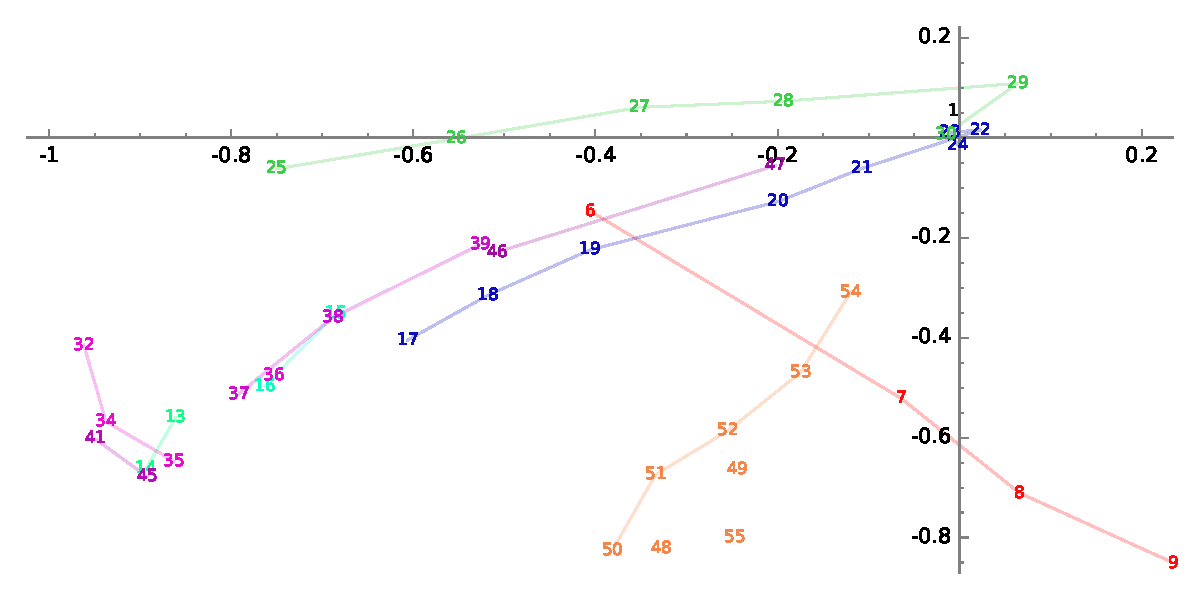
\includegraphics[width=0.95\linewidth]{figures/tableIDMLEStdErrZoomed.pdf}\\
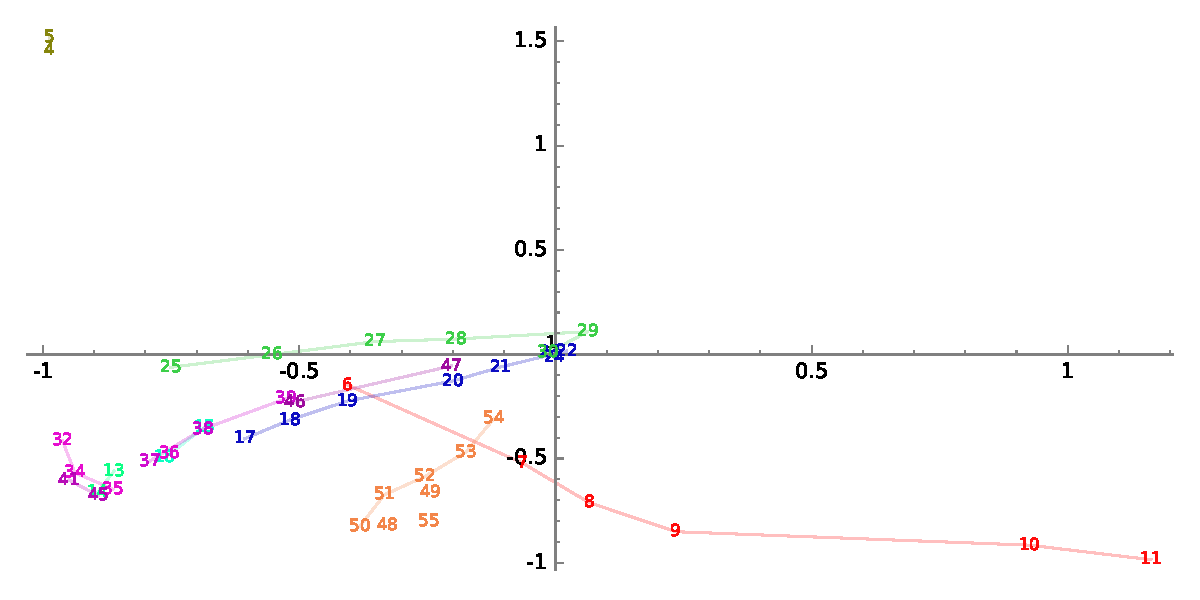
\includegraphics[width=0.95\linewidth]{figures/tableIDMLEStdErrZoomedOut.pdf}
\end{center}
\caption{A pictorial depiction of the mean MLEs $\overline{\hat{\alpha}}$ along x-axis and $\overline{\hat{\beta}}$ along y-axis based on transmission trees simulated from various contact networks indexed by their ID from \autoref{T:mles}.  Different IDs from the same parametric family are shown in the same color with lines connecting them if there is a natural parametric interpretation within the family (see description in text).  The top figure is a zoom-in of the bottom one.\label{F:tableIDMLEStdErrZoomed}}
\end{figure}

\subsection{Deterministic contact networks}
We have already seen the complete, path and star networks as our guiding examples in \autoref{S:Examples} and their corresponding exact Beta-splitting models in \autoref{S:Examples-betaSplitting}.  
We also saw that the unidirectional circular network is in the same effective Beta-splitting equivalence class as the path network in \autoref{S:UnidirectionalCircularNetwork}.  
In this section we explore a few key families of deterministic contact networks to further extend our insights by interpolations of the ones already seen, when possible.

\subsubsection{Bidirectional circular path network}
Let us extend the unidirectional circular network of \autoref{S:UnidirectionalCircularNetwork} to a bidirectional circular network by making each edge bidirected (or undirected).  
Thus $\{\imath_0,\imath_1,\ldots,\imath_{n-1}\}$ is the vertex set and 
$\{(\imath_0,\imath_1), (\imath_1,\imath_0), (\imath_1,\imath_2), (\imath_2,\imath_1), \ldots, (\imath_{n-1},\imath_{0}), (\imath_{0},\imath_{n-1})\}$ 
is the edge set for this bidirectional circular network.
With bidirectionality, we can have randomness in the transmission trees unlike the deterministic right-branching comb for the unidirectional case.  
This is because the next infection event can be either in the left or the right subtree of the root vertex encoding the first infection event.  
The initial infector could be any one of the vertices due to circular symmetry of the network and we take this to be $\imath_0$ without loss of generality.  
Thus the probability that the next infection is in the right or the left subtree of the root is equally likely, provided the current number of leaves (number of individuals infected) is less than $n$ and each edge-weight in this contact network is $1$.  
Finally each of these subtrees will be deterministically right-branching combs due to the fact that there is only one infected individual in each subtree that is capable of infecting its only uninfected out-neighbor, if any.  
We call such trees with {\em o}nly {\em r}ight-{\em b}ranching {\em s}ubtrees {\em o}f the {\em r}oot vertex as {\em orbsor} trees.  
Two such orbsor trees generated from the bidirectional contact network with $n=6$ and initialized from $\imath_0$ are shown in \autoref{F:bidirectionalCircular}. 

\begin{figure}[htbp]
\begin{center}
{\scalebox{0.95}{
%\begin{tabular}{cc}
\multirow{2}{*}[5em]{
{\scalebox{0.85}{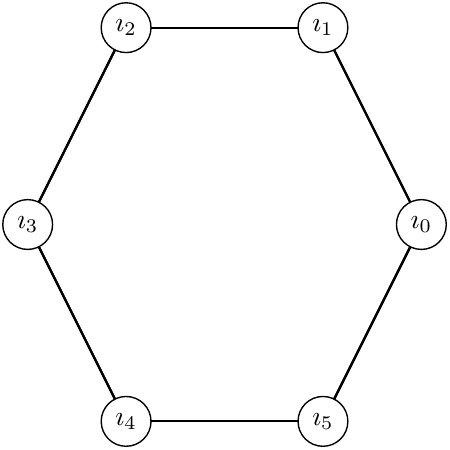
\begin{tikzpicture}
%
%\GraphInit[vstyle=Art]
%
\useasboundingbox (0,0) rectangle (5.0cm,5.0cm);
%
\Vertex[L=\hbox{$\imath_0$},x=5.0cm,y=2.5cm]{v0}
\Vertex[L=\hbox{$\imath_1$},x=3.75cm,y=5.0cm]{v1}
\Vertex[L=\hbox{$\imath_2$},x=1.25cm,y=5.0cm]{v2}
\Vertex[L=\hbox{$\imath_3$},x=0.0cm,y=2.5cm]{v3}
\Vertex[L=\hbox{$\imath_4$},x=1.25cm,y=0.0cm]{v4}
\Vertex[L=\hbox{$\imath_5$},x=3.75cm,y=0.0cm]{v5}
%
\Edge[](v0)(v1)
\Edge[](v0)(v5)
\Edge[](v1)(v0)
\Edge[](v1)(v2)
\Edge[](v2)(v1)
\Edge[](v2)(v3)
\Edge[](v3)(v2)
\Edge[](v3)(v4)
\Edge[](v4)(v3)
\Edge[](v4)(v5)
\Edge[](v5)(v0)
\Edge[](v5)(v4)
%
\end{tikzpicture}
}}}
&
{\scalebox{0.7}{ \newcommand{\nodea}{\node[draw,circle] (a) {$1$}
;}\newcommand{\nodeb}{\node[draw,circle] (b) {$3$}
;}\newcommand{\nodec}{\node[draw,circle] (c) {$\imath_0$}
;}\newcommand{\noded}{\node[draw,circle] (d) {$5$}
;}\newcommand{\nodee}{\node[draw,circle] (e) {$\imath_5$}
;}\newcommand{\nodef}{\node[draw,circle] (f) {$\imath_4$}
;}\newcommand{\nodeg}{\node[draw,circle] (g) {$2$}
;}\newcommand{\nodeh}{\node[draw,circle] (h) {$\imath_1$}
;}\newcommand{\nodei}{\node[draw,circle] (i) {$4$}
;}\newcommand{\nodej}{\node[draw,circle] (j) {$\imath_2$}
;}\newcommand{\nodeba}{\node[draw,circle] (ba) {$\imath_3$}
;}\begin{tikzpicture}[auto]
\matrix[column sep=.3cm, row sep=.3cm,ampersand replacement=\&]{
         \&         \&         \&         \&         \& \nodea  \&         \&         \&         \&         \&         \\ 
         \& \nodeb  \&         \&         \&         \&         \&         \& \nodeg  \&         \&         \&         \\ 
 \nodec  \&         \&         \& \noded  \&         \&         \& \nodeh  \&         \&         \& \nodei  \&         \\ 
         \&         \& \nodee  \&         \& \nodef  \&         \&         \&         \& \nodej  \&         \& \nodeba \\
};

\path[ultra thick, red] (d) edge (e) edge (f)
	(b) edge (c) edge (d)
	(i) edge (j) edge (ba)
	(g) edge (h) edge (i)
	(a) edge (b) edge (g);
\end{tikzpicture}}
}\\
~& {\scalebox{0.7}{ \newcommand{\nodea}{\node[draw,circle] (a) {$1$}
;}\newcommand{\nodeb}{\node[draw,circle] (b) {$2$}
;}\newcommand{\nodec}{\node[draw,circle] (c) {$\imath_0$}
;}\newcommand{\noded}{\node[draw,circle] (d) {$3$}
;}\newcommand{\nodee}{\node[draw,circle] (e) {$\imath_1$}
;}\newcommand{\nodef}{\node[draw,circle] (f) {$5$}
;}\newcommand{\nodeg}{\node[draw,circle] (g) {$\imath_2$}
;}\newcommand{\nodeh}{\node[draw,circle] (h) {$\imath_3$}
;}\newcommand{\nodei}{\node[draw,circle] (i) {$4$}
;}\newcommand{\nodej}{\node[draw,circle] (j) {$\imath_5$}
;}\newcommand{\nodeba}{\node[draw,circle] (ba) {$\imath_4$}
;}\begin{tikzpicture}[auto]
\matrix[column sep=.3cm, row sep=.3cm,ampersand replacement=\&]{
         \&         \&         \&         \&         \&         \&         \& \nodea  \&         \&         \&         \\ 
         \& \nodeb  \&         \&         \&         \&         \&         \&         \&         \& \nodei  \&         \\ 
 \nodec  \&         \&         \& \noded  \&         \&         \&         \&         \& \nodej  \&         \& \nodeba \\ 
         \&         \& \nodee  \&         \&         \& \nodef  \&         \&         \&         \&         \&         \\ 
         \&         \&         \&         \& \nodeg  \&         \& \nodeh  \&         \&         \&         \&         \\
};

\path[ultra thick, red] (f) edge (g) edge (h)
	(d) edge (e) edge (f)
	(b) edge (c) edge (d)
	(i) edge (j) edge (ba)
	(a) edge (b) edge (i);
\end{tikzpicture}}
}\\
\end{tabular}

\begin{tabular}{cc}
\multirow{2}{*}[5em]{
{\scalebox{0.85}{
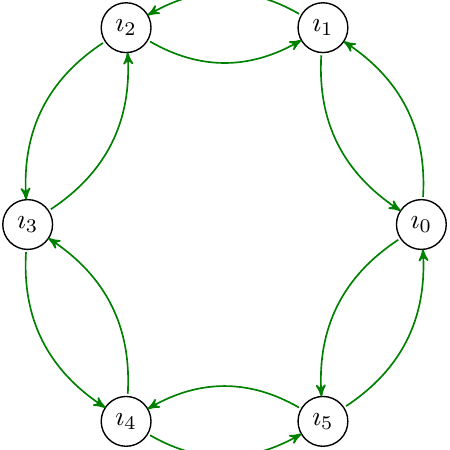
\begin{tikzpicture}
%
\useasboundingbox (0,0) rectangle (5.0cm,5.0cm);
%
\definecolor{cv0}{rgb}{0.0,0.502,0.0}
\definecolor{cfv0}{rgb}{1.0,1.0,1.0}
\definecolor{clv0}{rgb}{1.0,0.0,0.0}
\definecolor{cv1}{rgb}{0.0,0.502,0.0}
\definecolor{cfv1}{rgb}{1.0,1.0,1.0}
\definecolor{clv1}{rgb}{1.0,0.0,0.0}
\definecolor{cv2}{rgb}{0.0,0.502,0.0}
\definecolor{cfv2}{rgb}{1.0,1.0,1.0}
\definecolor{clv2}{rgb}{1.0,0.0,0.0}
\definecolor{cv3}{rgb}{0.0,0.502,0.0}
\definecolor{cfv3}{rgb}{1.0,1.0,1.0}
\definecolor{clv3}{rgb}{1.0,0.0,0.0}
\definecolor{cv4}{rgb}{0.0,0.502,0.0}
\definecolor{cfv4}{rgb}{1.0,1.0,1.0}
\definecolor{clv4}{rgb}{1.0,0.0,0.0}
\definecolor{cv5}{rgb}{0.0,0.502,0.0}
\definecolor{cfv5}{rgb}{1.0,1.0,1.0}
\definecolor{clv5}{rgb}{1.0,0.0,0.0}
\definecolor{cv0v1}{rgb}{0.0,0.502,0.0}
\definecolor{cv0v5}{rgb}{0.0,0.502,0.0}
\definecolor{cv1v0}{rgb}{0.0,0.502,0.0}
\definecolor{cv1v2}{rgb}{0.0,0.502,0.0}
\definecolor{cv2v1}{rgb}{0.0,0.502,0.0}
\definecolor{cv2v3}{rgb}{0.0,0.502,0.0}
\definecolor{cv3v2}{rgb}{0.0,0.502,0.0}
\definecolor{cv3v4}{rgb}{0.0,0.502,0.0}
\definecolor{cv4v3}{rgb}{0.0,0.502,0.0}
\definecolor{cv4v5}{rgb}{0.0,0.502,0.0}
\definecolor{cv5v0}{rgb}{0.0,0.502,0.0}
\definecolor{cv5v4}{rgb}{0.0,0.502,0.0}
%
\Vertex[style={minimum size=0.2cm,draw=cv0,fill=cfv0,text=clv0,shape=circle},LabelOut=false,L=\hbox{$\imath_0$},x=5.0cm,y=2.5cm]{v0}
\Vertex[style={minimum size=0.2cm,draw=cv1,fill=cfv1,text=clv1,shape=circle},LabelOut=false,L=\hbox{$\imath_1$},x=3.75cm,y=5.0cm]{v1}
\Vertex[style={minimum size=0.2cm,draw=cv2,fill=cfv2,text=clv2,shape=circle},LabelOut=false,L=\hbox{$\imath_2$},x=1.25cm,y=5.0cm]{v2}
\Vertex[style={minimum size=0.2cm,draw=cv3,fill=cfv3,text=clv3,shape=circle},LabelOut=false,L=\hbox{$\imath_3$},x=0.0cm,y=2.5cm]{v3}
\Vertex[style={minimum size=0.2cm,draw=cv4,fill=cfv4,text=clv4,shape=circle},LabelOut=false,L=\hbox{$\imath_4$},x=1.25cm,y=0.0cm]{v4}
\Vertex[style={minimum size=0.2cm,draw=cv5,fill=cfv5,text=clv5,shape=circle},LabelOut=false,L=\hbox{$\imath_5$},x=3.75cm,y=0.0cm]{v5}
%
\Edge[lw=0.04cm,style={post, bend right,color=cv0v1,},](v0)(v1)
\Edge[lw=0.04cm,style={post, bend right,color=cv0v5,},](v0)(v5)
\Edge[lw=0.04cm,style={post, bend right,color=cv1v0,},](v1)(v0)
\Edge[lw=0.04cm,style={post, bend right,color=cv1v2,},](v1)(v2)
\Edge[lw=0.04cm,style={post, bend right,color=cv2v1,},](v2)(v1)
\Edge[lw=0.04cm,style={post, bend right,color=cv2v3,},](v2)(v3)
\Edge[lw=0.04cm,style={post, bend right,color=cv3v2,},](v3)(v2)
\Edge[lw=0.04cm,style={post, bend right,color=cv3v4,},](v3)(v4)
\Edge[lw=0.04cm,style={post, bend right,color=cv4v3,},](v4)(v3)
\Edge[lw=0.04cm,style={post, bend right,color=cv4v5,},](v4)(v5)
\Edge[lw=0.04cm,style={post, bend right,color=cv5v0,},](v5)(v0)
\Edge[lw=0.04cm,style={post, bend right,color=cv5v4,},](v5)(v4)
%
\end{tikzpicture}
}}}
&
{\scalebox{0.7}{ \newcommand{\nodea}{\node[draw,circle] (a) {$1$}
;}\newcommand{\nodeb}{\node[draw,circle] (b) {$3$}
;}\newcommand{\nodec}{\node[draw,circle] (c) {$\imath_0$}
;}\newcommand{\noded}{\node[draw,circle] (d) {$5$}
;}\newcommand{\nodee}{\node[draw,circle] (e) {$\imath_5$}
;}\newcommand{\nodef}{\node[draw,circle] (f) {$\imath_4$}
;}\newcommand{\nodeg}{\node[draw,circle] (g) {$2$}
;}\newcommand{\nodeh}{\node[draw,circle] (h) {$\imath_1$}
;}\newcommand{\nodei}{\node[draw,circle] (i) {$4$}
;}\newcommand{\nodej}{\node[draw,circle] (j) {$\imath_2$}
;}\newcommand{\nodeba}{\node[draw,circle] (ba) {$\imath_3$}
;}\begin{tikzpicture}[auto]
\matrix[column sep=.3cm, row sep=.3cm,ampersand replacement=\&]{
         \&         \&         \&         \&         \& \nodea  \&         \&         \&         \&         \&         \\ 
         \& \nodeb  \&         \&         \&         \&         \&         \& \nodeg  \&         \&         \&         \\ 
 \nodec  \&         \&         \& \noded  \&         \&         \& \nodeh  \&         \&         \& \nodei  \&         \\ 
         \&         \& \nodee  \&         \& \nodef  \&         \&         \&         \& \nodej  \&         \& \nodeba \\
};

\path[ultra thick, red] (d) edge (e) edge (f)
	(b) edge (c) edge (d)
	(i) edge (j) edge (ba)
	(g) edge (h) edge (i)
	(a) edge (b) edge (g);
\end{tikzpicture}}
}\\
~& {\scalebox{0.7}{ \newcommand{\nodea}{\node[draw,circle] (a) {$1$}
;}\newcommand{\nodeb}{\node[draw,circle] (b) {$2$}
;}\newcommand{\nodec}{\node[draw,circle] (c) {$\imath_0$}
;}\newcommand{\noded}{\node[draw,circle] (d) {$3$}
;}\newcommand{\nodee}{\node[draw,circle] (e) {$\imath_1$}
;}\newcommand{\nodef}{\node[draw,circle] (f) {$5$}
;}\newcommand{\nodeg}{\node[draw,circle] (g) {$\imath_2$}
;}\newcommand{\nodeh}{\node[draw,circle] (h) {$\imath_3$}
;}\newcommand{\nodei}{\node[draw,circle] (i) {$4$}
;}\newcommand{\nodej}{\node[draw,circle] (j) {$\imath_5$}
;}\newcommand{\nodeba}{\node[draw,circle] (ba) {$\imath_4$}
;}\begin{tikzpicture}[auto]
\matrix[column sep=.3cm, row sep=.3cm,ampersand replacement=\&]{
         \&         \&         \&         \&         \&         \&         \& \nodea  \&         \&         \&         \\ 
         \& \nodeb  \&         \&         \&         \&         \&         \&         \&         \& \nodei  \&         \\ 
 \nodec  \&         \&         \& \noded  \&         \&         \&         \&         \& \nodej  \&         \& \nodeba \\ 
         \&         \& \nodee  \&         \&         \& \nodef  \&         \&         \&         \&         \&         \\ 
         \&         \&         \&         \& \nodeg  \&         \& \nodeh  \&         \&         \&         \&         \\
};

\path[ultra thick, red] (f) edge (g) edge (h)
	(d) edge (e) edge (f)
	(b) edge (c) edge (d)
	(i) edge (j) edge (ba)
	(a) edge (b) edge (i);
\end{tikzpicture}}
}\\
\end{tabular}

}}
\end{center}
\caption{The bidirectional circular contact network (left) and two sampled transmission trees from it (right).\label{F:bidirectionalCircular}}
\end{figure}

Putting all these facts together we can directly see that the probability distribution on transmission trees is uniformly distributed over the $2^{n-1}$ orbsor trees that form as subset of the $n!(n-1)!$ many possible transmission trees, as follows:
\begin{equation}\label{E:orbsorTransmissionTreeProb}
\Pr(\tau) = 
\begin{cases}
\frac{1}{2^{n-1}} & \text{ if $\tau$ is an orbsor tree with $n$ leaves},\\
0 & \text{ otherwise.}
\end{cases}
\end{equation}

For comparison with our three core examples, recall that the distribution on transmission trees induced by the complete, star and path networks are also uniformly distributed on the following subsets of the set of transmission trees: the entire set, the set of $(n-1)!$ left-branching comb trees and the singleton set of the right-branching comb tree, respectively.
Thus, our first four deterministic contact networks induce uniform distributions on various subsets of the set of all transmission trees.

As shown in \autoref{T:mles}, $(\overline{\widehat{\alpha}},\overline{\widehat{\beta}})$, the mean MLE of the effective Beta-splitting model based on $r=1$ or $r=100$ transmission trees drawn from such a network over $n=50$ individuals is close to $(-0.98,1.5)$.  
They are depicted by IDs 4 and 5 on the top left corner of the zoomed-out image at the bottom of \autoref{F:tableIDMLEStdErrZoomed}.  
Although some combinatorial book-keeping may allow one to analytically pursue the transformation of the distribution in \autoref{E:orbsorTransmissionTreeProb} to $\mathcal{S}_n$ (see last paragraph of \autoref{S:AnL1Perspective} and \autoref{S:D_TowardsOtherTreeResolutions}), we begin to content ourselves with mere simulation results in preparation for more complicated networks that are not easily amenable to extractions of exact expressions.  
The mean MLE of $(-0.98,1.5)$ for this bidirectional path network, that is binomially composing the right-branching comb of the path network on either side of its root vertex, makes intuitive sense because it is not as extreme as $(-1,\infty)$, the MLE of the path network at the boundary of the parameter space in its limit (with ID 3 that can be imagined in \autoref{F:tableIDMLEStdErrZoomed}).  

\subsubsection{Balanced tree network}

$\mathrm{BalancedTree}(d,h)$ is the perfectly balanced tree of height $h \geq 1$ and whose root has degree $d \geq 2$.  
The number of vertices in this network is $n = 1 + d + d^2 + \cdots + d^h = (d^{h+1} - 1)/(d - 1)$ and the number of edges is $n-1$.  
Balanced tree networks can be thought of as a biparametric extension of the star network which is equivalent to $\mathrm{BalancedTree}(n-1,1)$.  

\begin{figure}[htbp]
%\includegraphics[width=0.95\linewidth]{figures/leftSharks.pdf}
%{\resizebox{\textwidth}{!}{
\begin{center}
{\scalebox{0.85}{
\begin{tabular}{cc}
{\scalebox{0.55}
{
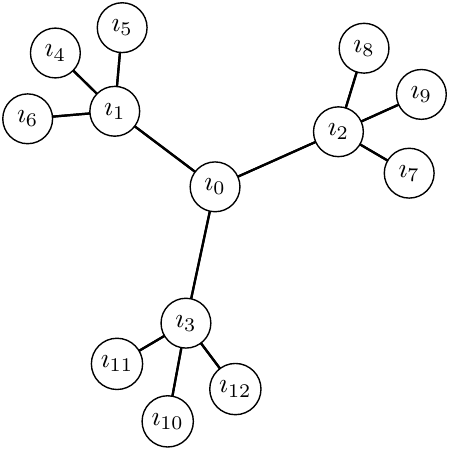
\begin{tikzpicture}
%
%\GraphInit[vstyle=Art]
%
\useasboundingbox (0,0) rectangle (5.0cm,5.0cm);
%
\Vertex[L=\hbox{$\imath_0$},x=2.3798cm,y=2.9787cm]{v0}
\Vertex[L=\hbox{$\imath_1$},x=1.106cm,y=3.9381cm]{v1}
\Vertex[L=\hbox{$\imath_2$},x=3.9466cm,y=3.6782cm]{v2}
\Vertex[L=\hbox{$\imath_3$},x=2.01cm,y=1.2471cm]{v3}
\Vertex[L=\hbox{$\imath_4$},x=0.3518cm,y=4.6782cm]{v4}
\Vertex[L=\hbox{$\imath_5$},x=1.2001cm,y=5.0cm]{v5}
\Vertex[L=\hbox{$\imath_6$},x=0.0cm,y=3.8427cm]{v6}
\Vertex[L=\hbox{$\imath_7$},x=4.8453cm,y=3.1519cm]{v7}
\Vertex[L=\hbox{$\imath_8$},x=4.272cm,y=4.739cm]{v8}
\Vertex[L=\hbox{$\imath_9$},x=5.0cm,y=4.1523cm]{v9}
\Vertex[L=\hbox{$\imath_{10}$},x=1.7786cm,y=0.0cm]{v10}
\Vertex[L=\hbox{$\imath_{11}$},x=1.1345cm,y=0.7302cm]{v11}
\Vertex[L=\hbox{$\imath_{12}$},x=2.6377cm,y=0.4102cm]{v12}
%
\Edge[](v0)(v1)
\Edge[](v0)(v2)
\Edge[](v0)(v3)
\Edge[](v1)(v0)
\Edge[](v1)(v4)
\Edge[](v1)(v5)
\Edge[](v1)(v6)
\Edge[](v2)(v0)
\Edge[](v2)(v7)
\Edge[](v2)(v8)
\Edge[](v2)(v9)
\Edge[](v3)(v0)
\Edge[](v3)(v10)
\Edge[](v3)(v11)
\Edge[](v3)(v12)
\Edge[](v4)(v1)
\Edge[](v5)(v1)
\Edge[](v6)(v1)
\Edge[](v7)(v2)
\Edge[](v8)(v2)
\Edge[](v9)(v2)
\Edge[](v10)(v3)
\Edge[](v11)(v3)
\Edge[](v12)(v3)
%
\end{tikzpicture}
}
}
&
{\scalebox{0.4}
{ \newcommand{\nodea}{\node[draw,circle] (a) {$1$}
;}\newcommand{\nodeb}{\node[draw,circle] (b) {$2$}
;}\newcommand{\nodec}{\node[draw,circle] (c) {$6$}
;}\newcommand{\noded}{\node[draw,circle] (d) {$\imath_0$}
;}\newcommand{\nodee}{\node[draw,circle] (e) {$7$}
;}\newcommand{\nodef}{\node[draw,circle] (f) {$8$}
;}\newcommand{\nodeg}{\node[draw,circle] (g) {$11$}
;}\newcommand{\nodeh}{\node[draw,circle] (h) {$\imath_2$}
;}\newcommand{\nodei}{\node[draw,circle] (i) {$\imath_8$}
;}\newcommand{\nodej}{\node[draw,circle] (j) {$\imath_7$}
;}\newcommand{\nodeba}{\node[draw,circle] (ba) {$\imath_9$}
;}\newcommand{\nodebb}{\node[draw,circle] (bb) {$3$}
;}\newcommand{\nodebc}{\node[draw,circle] (bc) {$4$}
;}\newcommand{\nodebd}{\node[draw,circle] (bd) {$10$}
;}\newcommand{\nodebe}{\node[draw,circle] (be) {$\imath_1$}
;}\newcommand{\nodebf}{\node[draw,circle] (bf) {$\imath_6$}
;}\newcommand{\nodebg}{\node[draw,circle] (bg) {$\imath_5$}
;}\newcommand{\nodebh}{\node[draw,circle] (bh) {$\imath_4$}
;}\newcommand{\nodebi}{\node[draw,circle] (bi) {$5$}
;}\newcommand{\nodebj}{\node[draw,circle] (bj) {$9$}
;}\newcommand{\nodeca}{\node[draw,circle] (ca) {$12$}
;}\newcommand{\nodecb}{\node[draw,circle] (cb) {$\imath_3$}
;}\newcommand{\nodecc}{\node[draw,circle] (cc) {$\imath_{11}$}
;}\newcommand{\nodecd}{\node[draw,circle] (cd) {$\imath_{10}$}
;}\newcommand{\nodece}{\node[draw,circle] (ce) {$\imath_{12}$}
;}\begin{tikzpicture}[auto]
\matrix[column sep=.3cm, row sep=.3cm,ampersand replacement=\&]{
         \&         \&         \&         \&         \&         \&         \&         \&         \&         \&         \&         \&         \&         \&         \&         \&         \& \nodea  \&         \&         \&         \&         \&         \&         \&         \\ 
         \&         \&         \&         \&         \&         \&         \&         \&         \& \nodeb  \&         \&         \&         \&         \&         \&         \&         \&         \&         \&         \&         \&         \&         \& \nodebi \&         \\ 
         \& \nodec  \&         \&         \&         \&         \&         \&         \&         \&         \&         \&         \&         \&         \&         \& \nodebb \&         \&         \&         \&         \&         \& \nodebj \&         \&         \& \nodece \\ 
 \noded  \&         \&         \&         \&         \&         \&         \& \nodee  \&         \&         \&         \&         \&         \& \nodebc \&         \&         \& \nodebh \&         \&         \& \nodeca \&         \&         \& \nodecd \&         \&         \\ 
         \&         \&         \&         \&         \& \nodef  \&         \&         \& \nodeba \&         \&         \& \nodebd \&         \&         \& \nodebg \&         \&         \&         \& \nodecb \&         \& \nodecc \&         \&         \&         \&         \\ 
         \&         \&         \& \nodeg  \&         \&         \& \nodej  \&         \&         \&         \& \nodebe \&         \& \nodebf \&         \&         \&         \&         \&         \&         \&         \&         \&         \&         \&         \&         \\ 
         \&         \& \nodeh  \&         \& \nodei  \&         \&         \&         \&         \&         \&         \&         \&         \&         \&         \&         \&         \&         \&         \&         \&         \&         \&         \&         \&         \\
};

\path[ultra thick, red] (g) edge (h) edge (i)
	(f) edge (g) edge (j)
	(e) edge (f) edge (ba)
	(c) edge (d) edge (e)
	(bd) edge (be) edge (bf)
	(bc) edge (bd) edge (bg)
	(bb) edge (bc) edge (bh)
	(b) edge (c) edge (bb)
	(ca) edge (cb) edge (cc)
	(bj) edge (ca) edge (cd)
	(bi) edge (bj) edge (ce)
	(a) edge (b) edge (bi);
\end{tikzpicture}}
}\\
~&~\\%\hline\\
~&~\\%\hline\\
{\scalebox{0.55}
{
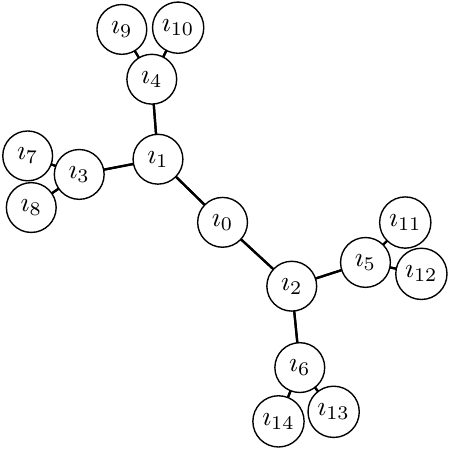
\begin{tikzpicture}
%
%\GraphInit[vstyle=Art]
%
\useasboundingbox (0,0) rectangle (5.0cm,5.0cm);
%
\Vertex[L=\hbox{$\imath_0$},x=2.4751cm,y=2.5278cm]{v0}
\Vertex[L=\hbox{$\imath_1$},x=1.6549cm,y=3.3293cm]{v1}
\Vertex[L=\hbox{$\imath_2$},x=3.3539cm,y=1.7168cm]{v2}
\Vertex[L=\hbox{$\imath_3$},x=0.6547cm,y=3.1362cm]{v3}
\Vertex[L=\hbox{$\imath_4$},x=1.5763cm,y=4.3456cm]{v4}
\Vertex[L=\hbox{$\imath_5$},x=4.29cm,y=2.0186cm]{v5}
\Vertex[L=\hbox{$\imath_6$},x=3.4558cm,y=0.683cm]{v6}
\Vertex[L=\hbox{$\imath_7$},x=0.0cm,y=3.3716cm]{v7}
\Vertex[L=\hbox{$\imath_8$},x=0.0456cm,y=2.7157cm]{v8}
\Vertex[L=\hbox{$\imath_9$},x=1.1962cm,y=4.9778cm]{v9}
\Vertex[L=\hbox{$\imath_{10}$},x=1.9111cm,y=5.0cm]{v10}
\Vertex[L=\hbox{$\imath_{11}$},x=4.7954cm,y=2.5252cm]{v11}
\Vertex[L=\hbox{$\imath_{12}$},x=5.0cm,y=1.8734cm]{v12}
\Vertex[L=\hbox{$\imath_{13}$},x=3.8858cm,y=0.1213cm]{v13}
\Vertex[L=\hbox{$\imath_{14}$},x=3.1853cm,y=0.0cm]{v14}
%
\Edge[](v0)(v1)
\Edge[](v0)(v2)
\Edge[](v1)(v0)
\Edge[](v1)(v3)
\Edge[](v1)(v4)
\Edge[](v2)(v0)
\Edge[](v2)(v5)
\Edge[](v2)(v6)
\Edge[](v3)(v1)
\Edge[](v3)(v7)
\Edge[](v3)(v8)
\Edge[](v4)(v1)
\Edge[](v4)(v9)
\Edge[](v4)(v10)
\Edge[](v5)(v2)
\Edge[](v5)(v11)
\Edge[](v5)(v12)
\Edge[](v6)(v2)
\Edge[](v6)(v13)
\Edge[](v6)(v14)
\Edge[](v7)(v3)
\Edge[](v8)(v3)
\Edge[](v9)(v4)
\Edge[](v10)(v4)
\Edge[](v11)(v5)
\Edge[](v12)(v5)
\Edge[](v13)(v6)
\Edge[](v14)(v6)
%
\end{tikzpicture}
}
}
&
{\scalebox{0.35}
{ \newcommand{\nodea}{\node[draw,circle] (a) {$1$}
;}\newcommand{\nodeb}{\node[draw,circle] (b) {$5$}
;}\newcommand{\nodec}{\node[draw,circle] (c) {$\imath_0$}
;}\newcommand{\noded}{\node[draw,circle] (d) {$6$}
;}\newcommand{\nodee}{\node[draw,circle] (e) {$7$}
;}\newcommand{\nodef}{\node[draw,circle] (f) {$\imath_1$}
;}\newcommand{\nodeg}{\node[draw,circle] (g) {$9$}
;}\newcommand{\nodeh}{\node[draw,circle] (h) {$13$}
;}\newcommand{\nodei}{\node[draw,circle] (i) {$\imath_4$}
;}\newcommand{\nodej}{\node[draw,circle] (j) {$\imath_{10}$}
;}\newcommand{\nodeba}{\node[draw,circle] (ba) {$\imath_9$}
;}\newcommand{\nodebb}{\node[draw,circle] (bb) {$10$}
;}\newcommand{\nodebc}{\node[draw,circle] (bc) {$14$}
;}\newcommand{\nodebd}{\node[draw,circle] (bd) {$\imath_3$}
;}\newcommand{\nodebe}{\node[draw,circle] (be) {$\imath_7$}
;}\newcommand{\nodebf}{\node[draw,circle] (bf) {$\imath_8$}
;}\newcommand{\nodebg}{\node[draw,circle] (bg) {$2$}
;}\newcommand{\nodebh}{\node[draw,circle] (bh) {$4$}
;}\newcommand{\nodebi}{\node[draw,circle] (bi) {$\imath_2$}
;}\newcommand{\nodebj}{\node[draw,circle] (bj) {$8$}
;}\newcommand{\nodeca}{\node[draw,circle] (ca) {$12$}
;}\newcommand{\nodecb}{\node[draw,circle] (cb) {$\imath_6$}
;}\newcommand{\nodecc}{\node[draw,circle] (cc) {$\imath_{14}$}
;}\newcommand{\nodecd}{\node[draw,circle] (cd) {$\imath_{13}$}
;}\newcommand{\nodece}{\node[draw,circle] (ce) {$3$}
;}\newcommand{\nodecf}{\node[draw,circle] (cf) {$11$}
;}\newcommand{\nodecg}{\node[draw,circle] (cg) {$\imath_5$}
;}\newcommand{\nodech}{\node[draw,circle] (ch) {$\imath_{12}$}
;}\newcommand{\nodeci}{\node[draw,circle] (ci) {$\imath_{11}$}
;}\begin{tikzpicture}[auto]
\matrix[column sep=.3cm, row sep=.3cm,ampersand replacement=\&]{
         \&         \&         \&         \&         \&         \&         \&         \&         \&         \&         \&         \&         \&         \&         \& \nodea  \&         \&         \&         \&         \&         \&         \&         \&         \&         \&         \&         \&         \&         \\ 
         \& \nodeb  \&         \&         \&         \&         \&         \&         \&         \&         \&         \&         \&         \&         \&         \&         \&         \&         \&         \&         \&         \&         \&         \& \nodebg \&         \&         \&         \&         \&         \\ 
 \nodec  \&         \&         \&         \&         \&         \&         \&         \&         \& \noded  \&         \&         \&         \&         \&         \&         \&         \& \nodebh \&         \&         \&         \&         \&         \&         \&         \&         \&         \& \nodece \&         \\ 
         \&         \&         \& \nodee  \&         \&         \&         \&         \&         \&         \&         \&         \&         \& \nodebb \&         \&         \& \nodebi \&         \&         \&         \&         \& \nodebj \&         \&         \&         \& \nodecf \&         \&         \& \nodeci \\ 
         \&         \& \nodef  \&         \&         \&         \&         \& \nodeg  \&         \&         \&         \& \nodebc \&         \&         \& \nodebf \&         \&         \&         \&         \& \nodeca \&         \&         \& \nodecd \&         \& \nodecg \&         \& \nodech \&         \&         \\ 
         \&         \&         \&         \&         \& \nodeh  \&         \&         \& \nodeba \&         \& \nodebd \&         \& \nodebe \&         \&         \&         \&         \&         \& \nodecb \&         \& \nodecc \&         \&         \&         \&         \&         \&         \&         \&         \\ 
         \&         \&         \&         \& \nodei  \&         \& \nodej  \&         \&         \&         \&         \&         \&         \&         \&         \&         \&         \&         \&         \&         \&         \&         \&         \&         \&         \&         \&         \&         \&         \\
};

\path[ultra thick, red] (h) edge (i) edge (j)
	(g) edge (h) edge (ba)
	(e) edge (f) edge (g)
	(bc) edge (bd) edge (be)
	(bb) edge (bc) edge (bf)
	(d) edge (e) edge (bb)
	(b) edge (c) edge (d)
	(ca) edge (cb) edge (cc)
	(bj) edge (ca) edge (cd)
	(bh) edge (bi) edge (bj)
	(cf) edge (cg) edge (ch)
	(ce) edge (cf) edge (ci)
	(bg) edge (bh) edge (ce)
	(a) edge (b) edge (bg);
\end{tikzpicture}}}\\
\end{tabular}

}}
\end{center}
\caption{The contact networks $\mathrm{BalancedTree}(3,2)$ (top left) and $\mathrm{BalancedTree}(2,3)$ (bottom left) and their corresponding transmission trees initialized from $\imath_0$ are given by the left-branching $3$-shark (top right) and $2$-shark (bottom right) trees, respectively\label{F:leftSharks}}
\end{figure}


The transmission tree generated on such perfectly balanced tree contact networks is unique if we ignore vertex labels and branch-lengths. 
We refer to them as left-branching $d$-sharks in the visual spirit of left-branching combs for star networks. 
Instead of giving a recursive formula for these trees we illustrate them by examples for $\mathrm{BalancedTree}(3,2)$ and $\mathrm{BalancedTree}(2,3)$ in \autoref{F:leftSharks}.
Thus, the $\mathrm{BalancedTree}(d,h)$ contact network produces a distribution on transmission trees that is concentrated on a single left-branching $d$-shark tree (ignoring all vertex labels and branch-lengths) and when $d=n-1$ and $h=1$ the left-branching $(n-1)$-shark tree is the left-branching comb tree for the star contact network.
The mean MLE of the effective Beta-splitting models are shown in \autoref{T:mles} for various values of $d$ and $h$.  
As $d$ and $h$ approach $n-1$ and $1$, respectively, while keeping the population size $n$ as close to $1000$ as possible, the corresponding mean MLEs are approaching $(\infty,-1)$, the limiting MLE of the star network with ID 2 and the $\mathrm{BalancedTree}(999,1)$ with ID 12 as expected.  
This tendency toward $(\infty,-1)$ is depicted by the sequence of IDs 6--11 in \autoref{F:tableIDMLEStdErrZoomed}.  
The standard errors are zero due to the uniqueness of the transmission tree (at the sufficient but not minimally sufficient resolution of rooted, unranked, planar and leaf-unlabelled tree) that is realized under each $\mathrm{BalancedTree}(d,h)$ contact network.
 
\subsubsection{Toroidal regular grid network}

We identify the vertices along the two pairs of opposite edges and the three pairs of opposite faces in the regular finite 2-dimensional (2D) square grid with $\sqrt{n} \times \sqrt{n}=n$ individual vertices and the 3-dimensional (3D) cube grid with $\sqrt[3]{n} \times \sqrt[3]{n} \times \sqrt[3]{n}=n$ individual vertices, respectively.  
A 2D toroidal grid with $n=9$ is shown in \autoref{F:toroidal2D}.  
The Figure also shows the sampling variation in three independent transmission trees grown on the network with initial infection at $\imath_0$.  

\begin{figure}[htbp]
\begin{center}
{\scalebox{0.725}{
\begin{tabular}{cc}
~&~\\
{\scalebox{0.70}{
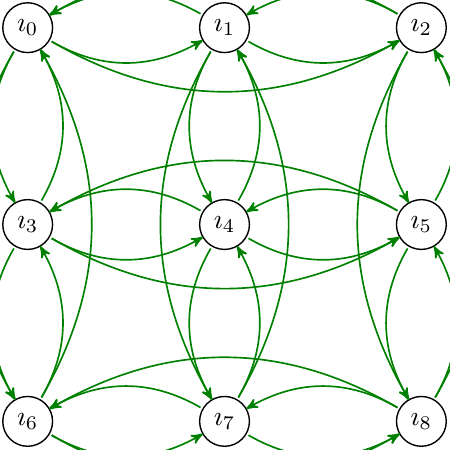
\begin{tikzpicture}
%
\useasboundingbox (0,0) rectangle (5.0cm,5.0cm);
%
\definecolor{cv0}{rgb}{0.0,0.502,0.0}
\definecolor{cfv0}{rgb}{1.0,1.0,1.0}
\definecolor{clv0}{rgb}{1.0,0.0,0.0}
\definecolor{cv1}{rgb}{0.0,0.502,0.0}
\definecolor{cfv1}{rgb}{1.0,1.0,1.0}
\definecolor{clv1}{rgb}{1.0,0.0,0.0}
\definecolor{cv2}{rgb}{0.0,0.502,0.0}
\definecolor{cfv2}{rgb}{1.0,1.0,1.0}
\definecolor{clv2}{rgb}{1.0,0.0,0.0}
\definecolor{cv3}{rgb}{0.0,0.502,0.0}
\definecolor{cfv3}{rgb}{1.0,1.0,1.0}
\definecolor{clv3}{rgb}{1.0,0.0,0.0}
\definecolor{cv4}{rgb}{0.0,0.502,0.0}
\definecolor{cfv4}{rgb}{1.0,1.0,1.0}
\definecolor{clv4}{rgb}{1.0,0.0,0.0}
\definecolor{cv5}{rgb}{0.0,0.502,0.0}
\definecolor{cfv5}{rgb}{1.0,1.0,1.0}
\definecolor{clv5}{rgb}{1.0,0.0,0.0}
\definecolor{cv6}{rgb}{0.0,0.502,0.0}
\definecolor{cfv6}{rgb}{1.0,1.0,1.0}
\definecolor{clv6}{rgb}{1.0,0.0,0.0}
\definecolor{cv7}{rgb}{0.0,0.502,0.0}
\definecolor{cfv7}{rgb}{1.0,1.0,1.0}
\definecolor{clv7}{rgb}{1.0,0.0,0.0}
\definecolor{cv8}{rgb}{0.0,0.502,0.0}
\definecolor{cfv8}{rgb}{1.0,1.0,1.0}
\definecolor{clv8}{rgb}{1.0,0.0,0.0}
\definecolor{cv0v1}{rgb}{0.0,0.502,0.0}
\definecolor{cv0v2}{rgb}{0.0,0.502,0.0}
\definecolor{cv0v3}{rgb}{0.0,0.502,0.0}
\definecolor{cv0v6}{rgb}{0.0,0.502,0.0}
\definecolor{cv1v0}{rgb}{0.0,0.502,0.0}
\definecolor{cv1v2}{rgb}{0.0,0.502,0.0}
\definecolor{cv1v4}{rgb}{0.0,0.502,0.0}
\definecolor{cv1v7}{rgb}{0.0,0.502,0.0}
\definecolor{cv2v0}{rgb}{0.0,0.502,0.0}
\definecolor{cv2v1}{rgb}{0.0,0.502,0.0}
\definecolor{cv2v5}{rgb}{0.0,0.502,0.0}
\definecolor{cv2v8}{rgb}{0.0,0.502,0.0}
\definecolor{cv3v0}{rgb}{0.0,0.502,0.0}
\definecolor{cv3v4}{rgb}{0.0,0.502,0.0}
\definecolor{cv3v5}{rgb}{0.0,0.502,0.0}
\definecolor{cv3v6}{rgb}{0.0,0.502,0.0}
\definecolor{cv4v1}{rgb}{0.0,0.502,0.0}
\definecolor{cv4v3}{rgb}{0.0,0.502,0.0}
\definecolor{cv4v5}{rgb}{0.0,0.502,0.0}
\definecolor{cv4v7}{rgb}{0.0,0.502,0.0}
\definecolor{cv5v2}{rgb}{0.0,0.502,0.0}
\definecolor{cv5v3}{rgb}{0.0,0.502,0.0}
\definecolor{cv5v4}{rgb}{0.0,0.502,0.0}
\definecolor{cv5v8}{rgb}{0.0,0.502,0.0}
\definecolor{cv6v0}{rgb}{0.0,0.502,0.0}
\definecolor{cv6v3}{rgb}{0.0,0.502,0.0}
\definecolor{cv6v7}{rgb}{0.0,0.502,0.0}
\definecolor{cv6v8}{rgb}{0.0,0.502,0.0}
\definecolor{cv7v1}{rgb}{0.0,0.502,0.0}
\definecolor{cv7v4}{rgb}{0.0,0.502,0.0}
\definecolor{cv7v6}{rgb}{0.0,0.502,0.0}
\definecolor{cv7v8}{rgb}{0.0,0.502,0.0}
\definecolor{cv8v2}{rgb}{0.0,0.502,0.0}
\definecolor{cv8v5}{rgb}{0.0,0.502,0.0}
\definecolor{cv8v6}{rgb}{0.0,0.502,0.0}
\definecolor{cv8v7}{rgb}{0.0,0.502,0.0}
%
\Vertex[style={minimum size=0.2cm,draw=cv0,fill=cfv0,text=clv0,shape=circle},LabelOut=false,L=\hbox{$\imath_0$},x=0.0cm,y=5.0cm]{v0}
\Vertex[style={minimum size=0.2cm,draw=cv1,fill=cfv1,text=clv1,shape=circle},LabelOut=false,L=\hbox{$\imath_1$},x=2.5cm,y=5.0cm]{v1}
\Vertex[style={minimum size=0.2cm,draw=cv2,fill=cfv2,text=clv2,shape=circle},LabelOut=false,L=\hbox{$\imath_2$},x=5.0cm,y=5.0cm]{v2}
\Vertex[style={minimum size=0.2cm,draw=cv3,fill=cfv3,text=clv3,shape=circle},LabelOut=false,L=\hbox{$\imath_3$},x=0.0cm,y=2.5cm]{v3}
\Vertex[style={minimum size=0.2cm,draw=cv4,fill=cfv4,text=clv4,shape=circle},LabelOut=false,L=\hbox{$\imath_4$},x=2.5cm,y=2.5cm]{v4}
\Vertex[style={minimum size=0.2cm,draw=cv5,fill=cfv5,text=clv5,shape=circle},LabelOut=false,L=\hbox{$\imath_5$},x=5.0cm,y=2.5cm]{v5}
\Vertex[style={minimum size=0.2cm,draw=cv6,fill=cfv6,text=clv6,shape=circle},LabelOut=false,L=\hbox{$\imath_6$},x=0.0cm,y=0.0cm]{v6}
\Vertex[style={minimum size=0.2cm,draw=cv7,fill=cfv7,text=clv7,shape=circle},LabelOut=false,L=\hbox{$\imath_7$},x=2.5cm,y=0.0cm]{v7}
\Vertex[style={minimum size=0.2cm,draw=cv8,fill=cfv8,text=clv8,shape=circle},LabelOut=false,L=\hbox{$\imath_8$},x=5.0cm,y=0.0cm]{v8}
%
\Edge[lw=0.04cm,style={post, bend right,color=cv0v1,},](v0)(v1)
\Edge[lw=0.04cm,style={post, bend right,color=cv0v2,},](v0)(v2)
\Edge[lw=0.04cm,style={post, bend right,color=cv0v3,},](v0)(v3)
\Edge[lw=0.04cm,style={post, bend right,color=cv0v6,},](v0)(v6)
\Edge[lw=0.04cm,style={post, bend right,color=cv1v0,},](v1)(v0)
\Edge[lw=0.04cm,style={post, bend right,color=cv1v2,},](v1)(v2)
\Edge[lw=0.04cm,style={post, bend right,color=cv1v4,},](v1)(v4)
\Edge[lw=0.04cm,style={post, bend right,color=cv1v7,},](v1)(v7)
\Edge[lw=0.04cm,style={post, bend right,color=cv2v0,},](v2)(v0)
\Edge[lw=0.04cm,style={post, bend right,color=cv2v1,},](v2)(v1)
\Edge[lw=0.04cm,style={post, bend right,color=cv2v5,},](v2)(v5)
\Edge[lw=0.04cm,style={post, bend right,color=cv2v8,},](v2)(v8)
\Edge[lw=0.04cm,style={post, bend right,color=cv3v0,},](v3)(v0)
\Edge[lw=0.04cm,style={post, bend right,color=cv3v4,},](v3)(v4)
\Edge[lw=0.04cm,style={post, bend right,color=cv3v5,},](v3)(v5)
\Edge[lw=0.04cm,style={post, bend right,color=cv3v6,},](v3)(v6)
\Edge[lw=0.04cm,style={post, bend right,color=cv4v1,},](v4)(v1)
\Edge[lw=0.04cm,style={post, bend right,color=cv4v3,},](v4)(v3)
\Edge[lw=0.04cm,style={post, bend right,color=cv4v5,},](v4)(v5)
\Edge[lw=0.04cm,style={post, bend right,color=cv4v7,},](v4)(v7)
\Edge[lw=0.04cm,style={post, bend right,color=cv5v2,},](v5)(v2)
\Edge[lw=0.04cm,style={post, bend right,color=cv5v3,},](v5)(v3)
\Edge[lw=0.04cm,style={post, bend right,color=cv5v4,},](v5)(v4)
\Edge[lw=0.04cm,style={post, bend right,color=cv5v8,},](v5)(v8)
\Edge[lw=0.04cm,style={post, bend right,color=cv6v0,},](v6)(v0)
\Edge[lw=0.04cm,style={post, bend right,color=cv6v3,},](v6)(v3)
\Edge[lw=0.04cm,style={post, bend right,color=cv6v7,},](v6)(v7)
\Edge[lw=0.04cm,style={post, bend right,color=cv6v8,},](v6)(v8)
\Edge[lw=0.04cm,style={post, bend right,color=cv7v1,},](v7)(v1)
\Edge[lw=0.04cm,style={post, bend right,color=cv7v4,},](v7)(v4)
\Edge[lw=0.04cm,style={post, bend right,color=cv7v6,},](v7)(v6)
\Edge[lw=0.04cm,style={post, bend right,color=cv7v8,},](v7)(v8)
\Edge[lw=0.04cm,style={post, bend right,color=cv8v2,},](v8)(v2)
\Edge[lw=0.04cm,style={post, bend right,color=cv8v5,},](v8)(v5)
\Edge[lw=0.04cm,style={post, bend right,color=cv8v6,},](v8)(v6)
\Edge[lw=0.04cm,style={post, bend right,color=cv8v7,},](v8)(v7)
%
\end{tikzpicture}
}}
&
{\scalebox{0.6}{
{ \newcommand{\nodea}{\node[draw,circle] (a) {$1$}
;}\newcommand{\nodeb}{\node[draw,circle] (b) {$2$}
;}\newcommand{\nodec}{\node[draw,circle] (c) {$3$}
;}\newcommand{\noded}{\node[draw,circle] (d) {$\imath_0$}
;}\newcommand{\nodee}{\node[draw,circle] (e) {$\imath_3$}
;}\newcommand{\nodef}{\node[draw,circle] (f) {$4$}
;}\newcommand{\nodeg}{\node[draw,circle] (g) {$6$}
;}\newcommand{\nodeh}{\node[draw,circle] (h) {$\imath_1$}
;}\newcommand{\nodei}{\node[draw,circle] (i) {$7$}
;}\newcommand{\nodej}{\node[draw,circle] (j) {$\imath_7$}
;}\newcommand{\nodeba}{\node[draw,circle] (ba) {$\imath_8$}
;}\newcommand{\nodebb}{\node[draw,circle] (bb) {$5$}
;}\newcommand{\nodebc}{\node[draw,circle] (bc) {$\imath_4$}
;}\newcommand{\nodebd}{\node[draw,circle] (bd) {$8$}
;}\newcommand{\nodebe}{\node[draw,circle] (be) {$\imath_5$}
;}\newcommand{\nodebf}{\node[draw,circle] (bf) {$\imath_2$}
;}\newcommand{\nodebg}{\node[draw,circle] (bg) {$\imath_6$}
;}\begin{tikzpicture}[auto]
\matrix[column sep=.3cm, row sep=.3cm,ampersand replacement=\&]{
         \&         \&         \&         \&         \&         \&         \&         \&         \&         \&         \&         \&         \&         \&         \& \nodea  \&         \\ 
         \&         \&         \& \nodeb  \&         \&         \&         \&         \&         \&         \&         \&         \&         \&         \&         \&         \& \nodebg \\ 
         \& \nodec  \&         \&         \&         \&         \&         \&         \&         \& \nodef  \&         \&         \&         \&         \&         \&         \&         \\ 
 \noded  \&         \& \nodee  \&         \&         \& \nodeg  \&         \&         \&         \&         \&         \& \nodebb \&         \&         \&         \&         \&         \\ 
         \&         \&         \&         \& \nodeh  \&         \&         \& \nodei  \&         \&         \& \nodebc \&         \&         \& \nodebd \&         \&         \&         \\ 
         \&         \&         \&         \&         \&         \& \nodej  \&         \& \nodeba \&         \&         \&         \& \nodebe \&         \& \nodebf \&         \&         \\
};

\path[ultra thick, red] (c) edge (d) edge (e)
	(i) edge (j) edge (ba)
	(g) edge (h) edge (i)
	(bd) edge (be) edge (bf)
	(bb) edge (bc) edge (bd)
	(f) edge (g) edge (bb)
	(b) edge (c) edge (f)
	(a) edge (b) edge (bg);
\end{tikzpicture}}
}}
\\
~&~\\
{\scalebox{0.38}{
{ \newcommand{\nodea}{\node[draw,circle] (a) {$1$}
;}\newcommand{\nodeb}{\node[draw,circle] (b) {$3$}
;}\newcommand{\nodec}{\node[draw,circle] (c) {$4$}
;}\newcommand{\noded}{\node[draw,circle] (d) {$6$}
;}\newcommand{\nodee}{\node[draw,circle] (e) {$\imath_0$}
;}\newcommand{\nodef}{\node[draw,circle] (f) {$\imath_6$}
;}\newcommand{\nodeg}{\node[draw,circle] (g) {$\imath_2$}
;}\newcommand{\nodeh}{\node[draw,circle] (h) {$\imath_3$}
;}\newcommand{\nodei}{\node[draw,circle] (i) {$2$}
;}\newcommand{\nodej}{\node[draw,circle] (j) {$5$}
;}\newcommand{\nodeba}{\node[draw,circle] (ba) {$\imath_1$}
;}\newcommand{\nodebb}{\node[draw,circle] (bb) {$7$}
;}\newcommand{\nodebc}{\node[draw,circle] (bc) {$\imath_7$}
;}\newcommand{\nodebd}{\node[draw,circle] (bd) {$\imath_8$}
;}\newcommand{\nodebe}{\node[draw,circle] (be) {$8$}
;}\newcommand{\nodebf}{\node[draw,circle] (bf) {$\imath_4$}
;}\newcommand{\nodebg}{\node[draw,circle] (bg) {$\imath_5$}
;}\begin{tikzpicture}[auto]
\matrix[column sep=.3cm, row sep=.3cm,ampersand replacement=\&]{
         \&         \&         \&         \&         \&         \&         \& \nodea  \&         \&         \&         \&         \&         \&         \&         \&         \&         \\ 
         \&         \&         \&         \&         \& \nodeb  \&         \&         \&         \&         \&         \&         \&         \& \nodei  \&         \&         \&         \\ 
         \&         \&         \& \nodec  \&         \&         \& \nodeh  \&         \&         \& \nodej  \&         \&         \&         \&         \&         \& \nodebe \&         \\ 
         \& \noded  \&         \&         \& \nodeg  \&         \&         \&         \& \nodeba \&         \&         \& \nodebb \&         \&         \& \nodebf \&         \& \nodebg \\ 
 \nodee  \&         \& \nodef  \&         \&         \&         \&         \&         \&         \&         \& \nodebc \&         \& \nodebd \&         \&         \&         \&         \\
};

\path[ultra thick, red] (d) edge (e) edge (f)
	(c) edge (d) edge (g)
	(b) edge (c) edge (h)
	(bb) edge (bc) edge (bd)
	(j) edge (ba) edge (bb)
	(be) edge (bf) edge (bg)
	(i) edge (j) edge (be)
	(a) edge (b) edge (i);
\end{tikzpicture}}
}}
&
{\scalebox{0.55}{
{ \newcommand{\nodea}{\node[draw,circle] (a) {$1$}
;}\newcommand{\nodeb}{\node[draw,circle] (b) {$8$}
;}\newcommand{\nodec}{\node[draw,circle] (c) {$\imath_0$}
;}\newcommand{\noded}{\node[draw,circle] (d) {$\imath_3$}
;}\newcommand{\nodee}{\node[draw,circle] (e) {$2$}
;}\newcommand{\nodef}{\node[draw,circle] (f) {$\imath_6$}
;}\newcommand{\nodeg}{\node[draw,circle] (g) {$3$}
;}\newcommand{\nodeh}{\node[draw,circle] (h) {$\imath_7$}
;}\newcommand{\nodei}{\node[draw,circle] (i) {$4$}
;}\newcommand{\nodej}{\node[draw,circle] (j) {$\imath_1$}
;}\newcommand{\nodeba}{\node[draw,circle] (ba) {$5$}
;}\newcommand{\nodebb}{\node[draw,circle] (bb) {$\imath_4$}
;}\newcommand{\nodebc}{\node[draw,circle] (bc) {$6$}
;}\newcommand{\nodebd}{\node[draw,circle] (bd) {$7$}
;}\newcommand{\nodebe}{\node[draw,circle] (be) {$\imath_5$}
;}\newcommand{\nodebf}{\node[draw,circle] (bf) {$\imath_8$}
;}\newcommand{\nodebg}{\node[draw,circle] (bg) {$\imath_2$}
;}\begin{tikzpicture}[auto]
\matrix[column sep=.3cm, row sep=.3cm,ampersand replacement=\&]{
         \&         \&         \& \nodea  \&         \&         \&         \&         \&         \&         \&         \&         \&         \&         \&         \&         \&         \\ 
         \& \nodeb  \&         \&         \&         \& \nodee  \&         \&         \&         \&         \&         \&         \&         \&         \&         \&         \&         \\ 
 \nodec  \&         \& \noded  \&         \& \nodef  \&         \&         \& \nodeg  \&         \&         \&         \&         \&         \&         \&         \&         \&         \\ 
         \&         \&         \&         \&         \&         \& \nodeh  \&         \&         \& \nodei  \&         \&         \&         \&         \&         \&         \&         \\ 
         \&         \&         \&         \&         \&         \&         \&         \& \nodej  \&         \&         \& \nodeba \&         \&         \&         \&         \&         \\ 
         \&         \&         \&         \&         \&         \&         \&         \&         \&         \& \nodebb \&         \&         \&         \&         \& \nodebc \&         \\ 
         \&         \&         \&         \&         \&         \&         \&         \&         \&         \&         \&         \&         \& \nodebd \&         \&         \& \nodebg \\ 
         \&         \&         \&         \&         \&         \&         \&         \&         \&         \&         \&         \& \nodebe \&         \& \nodebf \&         \&         \\
};

\path[ultra thick, red] (b) edge (c) edge (d)
	(bd) edge (be) edge (bf)
	(bc) edge (bd) edge (bg)
	(ba) edge (bb) edge (bc)
	(i) edge (j) edge (ba)
	(g) edge (h) edge (i)
	(e) edge (f) edge (g)
	(a) edge (b) edge (e);
\end{tikzpicture}}
}}
\end{tabular}

}}
\end{center}
\caption{Toroidal 2D grid contact network with $n=9$ (top left) and three sample transmission trees from it with initial infection at $\imath_0$.\label{F:toroidal2D}}
\end{figure}

Due to the toroidal structure, the transmission tree distributions are invariant to the initial infection (ignoring leaf labels).  
The mean MLEs of the effective Beta-splitting model corresponding to 2D and 3D toroidal grids with $n$ around $10^3$ and $10^4$ are depicted in \autoref{T:mles}.
The mean MLEs based on one transmission tree seem to be fairly concentrated about $(-0.9,-0.66)$ and $(-0.76,-0.5)$ for contact networks on toroidal 2D and 3D grids with about $n=10^4$ individuals, respectively.  
There is also an effect towards $(-1,-1)$ for the 2D and 3D cases as $n$ increases from about $10^3$ to $10^4$ as depicted by the ID pairs (13, 14) and (15,16) in \autoref{F:tableIDMLEStdErrZoomed}, respectively.

\subsection{Random contact networks}\label{S:RandomContactNetworks}

Although random graph models of contact networks add another level of randomness, 
we can informally think of a static contact network as a typical realization of a random network model \citep[Sec.~2.5]{AldousIPSSSD2013}.  
Thus the transmission process on any given static contact network can be used to provide insights into the sampling distribution of transmission trees for a large class of random network models already available in SageMath's graph libraries.
For example, the following code:

{\small
\begin{verbatim}
ts=[transmissionProcessTC(graphs.RandomRegular(k,n).to_directed(),0) 
                                                    for _ in range(1000)]
\end{verbatim}
}
\noindent
can produce $1000$ independent samples of transmission trees from $1000$ independent realizations of the random $k$-regular graph over $n$ vertices. 
We explore some basic random graph models to gain insights into the distribution of transmission trees and the MLEs of their effective Beta-splitting models.  

\begin{remark}
Let us note that one may also study the distribution of transmission trees for a specific realization of a given random contact network or its partially observed sub-network.  
Such subtle distinctions, which in turn will depend on the exact decision problem and the available data at hand, can be pursued by modifying our basic code in \autoref{sec:Code}.  
But here we limit ourselves to the random sense involving multiple independent trials such that each trial is a realization of a full transmission tree with $n$ leaves on each realization of a given random contact network with an initially infected node (i.e., a static initial SICN). 
\end{remark}
 
\subsubsection{Erd\H{o}s-R\'enyi random network}

The Erd\H{o}s-R\'enyi random network denoted by $\mathrm{ER}(n,p)$ on $n$ vertices is obtained by inserting each of the $n(n-1)/2$ undirected edges independently with probability $p$ \citep{Erdos1959,gilbert1959}.  
We interpret the undirected edges as being bidirected to obtain our random contact network $\mathrm{ER}(n,p)$ to study transmission trees evolving on the connected component of $\mathrm{ER}(n,p)$ containing the initially infected individual $\imath_0$.  
Thus $\mathrm{ER}(n,p)$ becomes more dense and approaches the complete network as the edge probability $p \to 1$ or equivalently as the average vertex degree $\lambda :=np \to n$.  
We observed more than $90$ vertices on average in the connected component containing $\imath_0$ if $p>0.03$ when $n=100$.  
This is sensible because $\mathrm{ER}(n,p)$ is known theoretically to have a unique giant component containing a positive fraction of the vertices almost surely if $\lambda>1$.  %; but this giant component need not necessarily contain our fixed vertex $\imath_0$. 
We are primarily interested in the regime where $p>\log(n)/n = \log(100)/100\approxeq 0.0461$ (in \autoref{T:mles}) or $\lambda>\log(100)\approxeq 4.61$ (in \autoref{F:MLE_ERRG_n100_r30_samp2}) when $\mathrm{ER}(n,p)$ is known theoretically to be connected almost surely so that all $n$ individuals can be eventually infected from the initial infection at $\imath_0$. 

Maximum likelihood estimates $\widehat{\alpha}$ and $\widehat{\beta}$ of the effective Beta-splitting model 
based on $r=30$ independent transmission trees that were grown on independent realizations of $\mathrm{ER}(100,\lambda/100)$ and replicated in five independent trials are shown in \autoref{F:MLE_ERRG_n100_r30_samp2} as a function of $\lambda$.   
The mean and standard errors of the MLEs are also given in \autoref{T:mles}.  
Note that the standard errors are higher when compared to those of the deterministic contact networks if $r=1$ (results not shown).  
This is naturally due to the additional randomness introduced by distinct realizations of the $\mathrm{ER}(n,p)$ random contact network across the trials.  
The standard errors in \autoref{T:mles} have been reduced by increasing $r$ to $30$.  
As expected, the MLEs plotted as points in \autoref{F:MLE_ERRG_n100_r30_samp2} and the mean MLEs in \autoref{T:mles} and their corresponding IDs 17--24 in \autoref{F:tableIDMLEStdErrZoomed} approach the origin as $\lambda$ approaches $100$ and the contact network $\mathrm{ER}(100,1)$ becomes the complete network.

Interestingly ID 6 of the deterministic $\mathrm{BalancedTree}(2,9)$ has its MLE fairly close to the mean MLE of $\mathrm{ER}(100,0.050)$ with ID 19.  
When $h$ is increased by $1$ from $6$ (with $n=127$) to $9$ (with $n=1023$), the mean MLE of $\mathrm{BalancedTree}(2,9)$ starts from $(-0.3259, -0.05752)$ and reaches $(-0.4052, -0.1477)$ piece-wise linearly with different slopes slightly over $1$.  
These results are in sync with a standard probability trick of approximating a sparse connected $\mathrm{ER}$ using trees.  
\begin{figure}[htbp]
\begin{center}
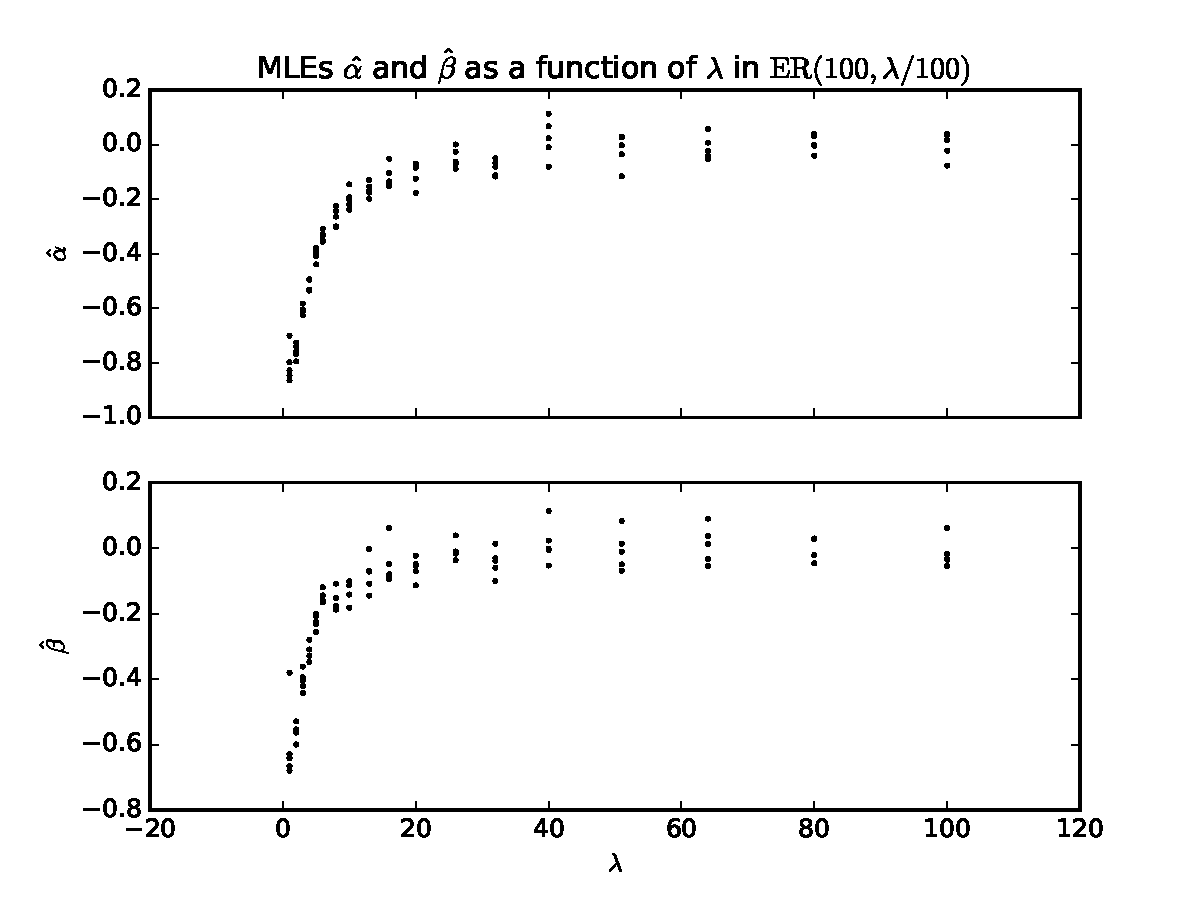
\includegraphics[width=0.95\linewidth]{figures/MLE_ERRG_n100_r30_samp2.pdf}
\end{center}
\caption{The Maximum likelihood estimates $\hat{\alpha}$ and $\hat{\beta}$ as a function of average vertex degree $\lambda$ in the Erd\H{o}s-R\'enyi random network $\mathrm{ER}(n,p)$ on $n=100$ vertices with edge probability $p=\lambda/n$. The estimates are based on $r=30$ independent transmission trees grown on independent realizations of $\mathrm{ER}(100,\lambda/100)$ in five replicate trials.\label{F:MLE_ERRG_n100_r30_samp2}}
\end{figure}

%\subsubsection{Erased configuration random graph} % too much man...

\subsubsection{Random regular network}
Each vertex in a {\em $d$-regular graph} has the same degree $d$ or number of neighbors.
A $d$-regular directed graph or network must also satisfy the stronger condition that the indegree and outdegree of each vertex are equal to each other. 
A random $d$-regular graph is a graph drawn uniformly at random from the set of all $d$-regular graphs on $n$ vertices, 
where $3 \leq d < n$ and $nd$ is even \citep{BollabosRGBook2001}.  
%Since every edge is incident to two vertices, $nd$ must be even.  
We merely interpret the undirected edges as being bidirected to obtain $\mathrm{RandReg}(n,d)$, the random $d$-regular network on $n$ vertices.  
Note that $\mathrm{RandReg}(n,d)$ approaches the complete network on $n$ vertices as $d$ approaches $n-1$.  
This is evident in the behavior of the mean MLEs obtained from $r=1$ transmission tree grown on the $\mathrm{RandReg}(n,d)$ contact network on $n=1000$ vertices for values of $d$ in $\{3,4,6,10,100,999\}$ as shown in \autoref{T:mles} and by their IDs 25--30 approaching ID 0 of the complete network with the same $n$ and $r$ at the origin in \autoref{F:tableIDMLEStdErrZoomed}.  
Note that Model ID 28 with $d=10$ and $n=1000$ nearly satisfies the condition that $d = O(n^{1/3 - \epsilon})$ 
for the underlying randomized algorithm \citep{StegerWormald1999} to generate an asymptotically uniform random $d$-regular graph on $n$ vertices \citep{KimVu2003}.

\subsubsection{Connected small-world random network}

The small-world random graph model of \cite{watts1998} on $n$ vertices is constructed by first creating a ring over $n$ vertices (undirected circular path graph).
Then each vertex in the ring is connected with its $m$ nearest neighbors if $m$ is even (and its $m-1$ nearest neighbors if $m$ is odd). 
Finally edges are rewired as follows: for each edge $(u,v)$ in the underlying {\em $n$-ring with $m$ nearest neighbors} graph, 
with probability $p$ rewire $(u,v)$ as the new edge $(u,w)$ with randomly-chosen existing vertex $w$. 
The undirected edges are interpreted as bidirected and we repeatedly sample until we obtain a {\em connected small world random network} $\mathrm{SWRN}(n,m,q)$ that is specified by the three parameters: $n$ for the number of vertices, 
$m$ for the number of nearest neighbors each vertex is connected to and $q$ for the probability of rewiring each edge.  
Thus, $\mathrm{SWRN}(n,m,q)$  accounts for clustering and at least partially explains the ``small-world'' phenomena that is observed in a variety of real-world networks while retaining the short average path lengths of the Erd\H{o}s-R\'enyi random graph $\mathrm{ER}(n,p)$.  

We consider two possible initializations, i.e.~two different initial SICNs for a given realization of $\mathrm{SWRN}(n,m,q)$.  
In the first case, denoted by $\mathrm{SWRN}^*(n,m,q)$, we grow the transmission tree from the vertex with the largest out-degree.  
If more than one vertex has the maximal out-degree then we choose the vertex with the smallest label.  
In the second case, denoted by $\mathrm{SWRN}^{\circ}(n,m,q)$, we grow the transmission tree from a randomly chosen vertex.  
The maximum likelihood estimates for their effective Beta-splitting models are obtained from $r$ independent transmission trees grown on these random networks with the two initializations having different parameters as shown in \autoref{T:mles} with their IDs.  
The two initializations basically coincide when $q=0$.  

We mainly explore the case with $m$ equalling $2$ and $5$ with $1$ and $2$ neighbors, respectively, on either side of each vertex initially, for a few values of the rewiring probability $q \in \{0.2,0.5,0.99\}$ with $n\in\{50,100\}$ and $r \in \{1,30\}$ as shown in \autoref{T:mles} and depicted with their IDs 31--47 in \autoref{F:tableIDMLEStdErrZoomed}.  
More interpretable IDs, in the sense of having variation in only one parameter in the family, are shown by the same color with lines connecting them.  

$\mathrm{SWRN}(n,m,q)$ interpolates between the {\em $n$-ring with $m$ nearest neighbors} network and $\mathrm{ER}(n,p)$, 
such that, as $q \to 1$, $\mathrm{SWRN}(n,m,q) \to \mathrm{ER}\left(n, nm/(n(n-1))\right)$.
When $q$ is close to $1$, we do find that the MLEs of $\mathrm{SWRN}^{\circ}(100,5,0.99)$ with ID 46, with initial infection chosen uniformly at random just as in the $\mathrm{ER}(n,p)$ contact network, are roughly closer to those for 
$\mathrm{ER}(100,0.050)$ with ID 19 since $nm/(n(n-1)) \approxeq 0.05$ when compared with $\mathrm{SWRN}^{\circ}(100,5,q)$ with smaller values of $q$ (results not shown).  

An interesting observation is the proximity of the mean MLEs for certain 2D and 3D toroidal grids to certain $\mathrm{SWRN}$s: (i) ID 15 of the 3D toroidal grid with $n=1000$ vertices (each connected to its six nearest neighbors) and ID 38 of $\mathrm{SWRN}^{\circ}(50,5,0.2)$ (each of its $50$ vertices initially connected to its four nearest neighbors before being rewired with probability $0.2$), (ii) ID 16 of the 3D toroidal grid with $n=10648$ and IDs 36 and 37 corresponding to $\mathrm{SWRN}^{*}(50,5,0.1)$ and $\mathrm{SWRN}^{\circ}(50,5,0.1)$, respectively, and (iii) ID 14 of the 2D toroidal grid with $n=10^4$ and $\mathrm{SWRN}^{\circ}(100,2,0.5)$ with ID 45.  
More extensive simulations are necessary to systematically understand these proximities (using rigorous global interval optimization techniques, say in \cite{HofschusterK03}, for the MLEs as opposed to the local optimizations used here).  
Insights from such rigorous simulations may lead to further analysis towards understanding the nature of such proximities between these distinct model families under the Beta-projections of \autoref{E:Thm3E3}, especially for different values of $n$.  
Other insights from \autoref{F:tableIDMLEStdErrZoomed} include the effect of changing $n$ and the initialization strategy.

%TODO add this to the public sagemathcloudworksheet from the rough one

\subsubsection{Preferential attachment random network}

Next we explore the random network created using the preferential attachment model of \cite{Barabasi1999}.  
Real-world networks are best described by a scale-free power-law distribution for their degrees. 
The preferential attachment model, unlike the other random graph models here, produces such a power-law degree distribution through two generic mechanisms: (i) networks are grown by the addition of new vertices, and (ii) new vertices attach preferentially to exiting vertices that are already well connected (i.e. with a high degree). 
The randomized algorithm for the construction of the preferential attachment network $\mathrm{PrefAttach}(n,m)$ is as follows.  
First, a graph with $m$ vertices and no edges is initialized, and a graph of $n$ vertices is grown by attaching new vertices, each with $m$ edges, 
to existing vertices independently according to probability proportional to their degrees.  
This results in a preferential attachment behavior whereby new vertices are attached to existing vertices that already have a high degree.  
We interpret the undirected edges as bidirected to obtain a network.  

\begin{figure}[htbp]
\begin{center}
{\scalebox{0.95}{
{\scalebox{0.375}{
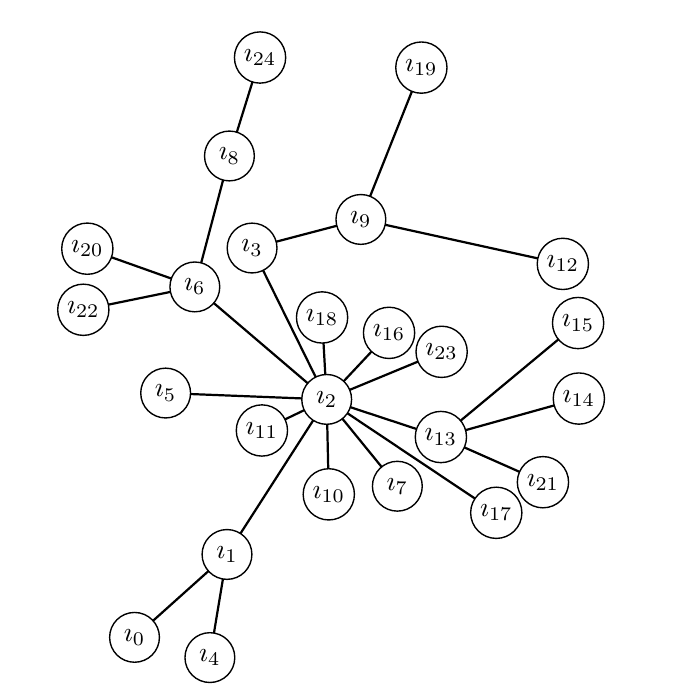
\begin{tikzpicture}
%
%\GraphInit[vstyle=Art]
%
\useasboundingbox (0,0) rectangle (8.0cm,8.0cm);
%
\Vertex[L=\hbox{$\imath_0$},x=1.357cm,y=0.2571cm]{v0}
\Vertex[L=\hbox{$\imath_1$},x=2.5314cm,y=1.3099cm]{v1}
\Vertex[L=\hbox{$\imath_2$},x=3.7974cm,y=3.2791cm]{v2}
\Vertex[L=\hbox{$\imath_3$},x=2.85cm,y=5.2013cm]{v3}
\Vertex[L=\hbox{$\imath_4$},x=2.314cm,y=0.0cm]{v4}
\Vertex[L=\hbox{$\imath_5$},x=1.7522cm,y=3.3596cm]{v5}
\Vertex[L=\hbox{$\imath_6$},x=2.123cm,y=4.7076cm]{v6}
\Vertex[L=\hbox{$\imath_7$},x=4.6948cm,y=2.1764cm]{v7}
\Vertex[L=\hbox{$\imath_8$},x=2.5623cm,y=6.3705cm]{v8}
\Vertex[L=\hbox{$\imath_9$},x=4.2317cm,y=5.5645cm]{v9}
\Vertex[L=\hbox{$\imath_{10}$},x=3.8242cm,y=2.0733cm]{v10}
\Vertex[L=\hbox{$\imath_{11}$},x=2.9747cm,y=2.8843cm]{v11}
\Vertex[L=\hbox{$\imath_{12}$},x=6.7967cm,y=5.0cm]{v12}
\Vertex[L=\hbox{$\imath_{13}$},x=5.2479cm,y=2.8012cm]{v13}
\Vertex[L=\hbox{$\imath_{14}$},x=7.0cm,y=3.2897cm]{v14}
\Vertex[L=\hbox{$\imath_{15}$},x=6.9906cm,y=4.2488cm]{v15}
\Vertex[L=\hbox{$\imath_{16}$},x=4.5896cm,y=4.1241cm]{v16}
\Vertex[L=\hbox{$\imath_{17}$},x=5.9511cm,y=1.8389cm]{v17}
\Vertex[L=\hbox{$\imath_{18}$},x=3.739cm,y=4.3199cm]{v18}
\Vertex[L=\hbox{$\imath_{19}$},x=5.0cm,y=7.4928cm]{v19}
\Vertex[L=\hbox{$\imath_{20}$},x=0.7577cm,y=5.1931cm]{v20}
\Vertex[L=\hbox{$\imath_{21}$},x=6.544cm,y=2.2274cm]{v21}
\Vertex[L=\hbox{$\imath_{22}$},x=0.7065cm,y=4.4172cm]{v22}
\Vertex[L=\hbox{$\imath_{23}$},x=5.2572cm,y=3.8833cm]{v23}
\Vertex[L=\hbox{$\imath_{24}$},x=2.9512cm,y=7.6209cm]{v24}
%
\Edge[](v0)(v1)
\Edge[](v1)(v2)
\Edge[](v1)(v4)
\Edge[](v2)(v3)
\Edge[](v2)(v5)
\Edge[](v2)(v6)
\Edge[](v2)(v7)
\Edge[](v2)(v10)
\Edge[](v2)(v11)
\Edge[](v2)(v13)
\Edge[](v2)(v16)
\Edge[](v2)(v17)
\Edge[](v2)(v18)
\Edge[](v2)(v23)
\Edge[](v3)(v9)
\Edge[](v6)(v8)
\Edge[](v6)(v20)
\Edge[](v6)(v22)
\Edge[](v8)(v24)
\Edge[](v9)(v12)
\Edge[](v9)(v19)
\Edge[](v13)(v14)
\Edge[](v13)(v15)
\Edge[](v13)(v21)
%
\end{tikzpicture}
}}
{\scalebox{0.19}{
{ \newcommand{\nodea}{\node[draw,circle] (a) {$1$}
;}\newcommand{\nodeb}{\node[draw,circle] (b) {$2$}
;}\newcommand{\nodec}{\node[draw,circle] (c) {$3$}
;}\newcommand{\noded}{\node[draw,circle] (d) {$4$}
;}\newcommand{\nodee}{\node[draw,circle] (e) {$6$}
;}\newcommand{\nodef}{\node[draw,circle] (f) {$7$}
;}\newcommand{\nodeg}{\node[draw,circle] (g) {$8$}
;}\newcommand{\nodeh}{\node[draw,circle] (h) {$9$}
;}\newcommand{\nodei}{\node[draw,circle] (i) {$10$}
;}\newcommand{\nodej}{\node[draw,circle] (j) {$12$}
;}\newcommand{\nodeba}{\node[draw,circle] (ba) {$14$}
;}\newcommand{\nodebb}{\node[draw,circle] (bb) {$16$}
;}\newcommand{\nodebc}{\node[draw,circle] (bc) {$\imath_2$}
;}\newcommand{\nodebd}{\node[draw,circle] (bd) {$\imath_{18}$}
;}\newcommand{\nodebe}{\node[draw,circle] (be) {$15$}
;}\newcommand{\nodebf}{\node[draw,circle] (bf) {$20$}
;}\newcommand{\nodebg}{\node[draw,circle] (bg) {$24$}
;}\newcommand{\nodebh}{\node[draw,circle] (bh) {$\imath_{13}$}
;}\newcommand{\nodebi}{\node[draw,circle] (bi) {$\imath_{14}$}
;}\newcommand{\nodebj}{\node[draw,circle] (bj) {$\imath_{15}$}
;}\newcommand{\nodeca}{\node[draw,circle] (ca) {$\imath_{21}$}
;}\newcommand{\nodecb}{\node[draw,circle] (cb) {$17$}
;}\newcommand{\nodecc}{\node[draw,circle] (cc) {$19$}
;}\newcommand{\nodecd}{\node[draw,circle] (cd) {$\imath_1$}
;}\newcommand{\nodece}{\node[draw,circle] (ce) {$\imath_4$}
;}\newcommand{\nodecf}{\node[draw,circle] (cf) {$\imath_0$}
;}\newcommand{\nodecg}{\node[draw,circle] (cg) {$18$}
;}\newcommand{\nodech}{\node[draw,circle] (ch) {$\imath_3$}
;}\newcommand{\nodeci}{\node[draw,circle] (ci) {$22$}
;}\newcommand{\nodecj}{\node[draw,circle] (cj) {$23$}
;}\newcommand{\nodeda}{\node[draw,circle] (da) {$\imath_9$}
;}\newcommand{\nodedb}{\node[draw,circle] (db) {$\imath_{12}$}
;}\newcommand{\nodedc}{\node[draw,circle] (dc) {$\imath_{19}$}
;}\newcommand{\nodedd}{\node[draw,circle] (dd) {$\imath_{17}$}
;}\newcommand{\nodede}{\node[draw,circle] (de) {$\imath_{16}$}
;}\newcommand{\nodedf}{\node[draw,circle] (df) {$\imath_{10}$}
;}\newcommand{\nodedg}{\node[draw,circle] (dg) {$\imath_5$}
;}\newcommand{\nodedh}{\node[draw,circle] (dh) {$\imath_{11}$}
;}\newcommand{\nodedi}{\node[draw,circle] (di) {$5$}
;}\newcommand{\nodedj}{\node[draw,circle] (dj) {$13$}
;}\newcommand{\nodeea}{\node[draw,circle] (ea) {$21$}
;}\newcommand{\nodeeb}{\node[draw,circle] (eb) {$\imath_6$}
;}\newcommand{\nodeec}{\node[draw,circle] (ec) {$\imath_{20}$}
;}\newcommand{\nodeed}{\node[draw,circle] (ed) {$\imath_{22}$}
;}\newcommand{\nodeee}{\node[draw,circle] (ee) {$11$}
;}\newcommand{\nodeef}{\node[draw,circle] (ef) {$\imath_8$}
;}\newcommand{\nodeeg}{\node[draw,circle] (eg) {$\imath_{24}$}
;}\newcommand{\nodeeh}{\node[draw,circle] (eh) {$\imath_{23}$}
;}\newcommand{\nodeei}{\node[draw,circle] (ei) {$\imath_7$}
;}\begin{tikzpicture}[auto]
\matrix[column sep=.3cm, row sep=.3cm,ampersand replacement=\&]{
         \&         \&         \&         \&         \&         \&         \&         \&         \&         \&         \&         \&         \&         \&         \&         \&         \&         \&         \&         \&         \&         \&         \&         \&         \&         \&         \&         \&         \&         \&         \&         \&         \&         \&         \&         \&         \&         \&         \&         \&         \&         \&         \&         \&         \&         \&         \& \nodea  \&         \\ 
         \&         \&         \&         \&         \&         \&         \&         \&         \&         \&         \&         \&         \&         \&         \&         \&         \&         \&         \&         \&         \&         \&         \&         \&         \&         \&         \&         \&         \&         \&         \&         \&         \&         \&         \&         \&         \&         \&         \&         \&         \&         \&         \&         \&         \& \nodeb  \&         \&         \& \nodeei \\ 
         \&         \&         \&         \&         \&         \&         \&         \&         \&         \&         \&         \&         \&         \&         \&         \&         \&         \&         \&         \&         \&         \&         \&         \&         \&         \&         \&         \&         \&         \&         \&         \&         \&         \&         \& \nodec  \&         \&         \&         \&         \&         \&         \&         \&         \&         \&         \& \nodeeh \&         \&         \\ 
         \&         \&         \&         \&         \&         \&         \&         \&         \&         \&         \&         \&         \&         \&         \&         \&         \&         \&         \&         \&         \&         \&         \&         \&         \&         \&         \&         \&         \&         \&         \&         \&         \& \noded  \&         \&         \&         \&         \&         \&         \&         \& \nodedi \&         \&         \&         \&         \&         \&         \&         \\ 
         \&         \&         \&         \&         \&         \&         \&         \&         \&         \&         \&         \&         \&         \&         \&         \&         \&         \&         \&         \&         \&         \&         \&         \&         \&         \&         \&         \&         \&         \&         \& \nodee  \&         \&         \& \nodedh \&         \&         \&         \&         \& \nodedj \&         \&         \&         \& \nodeee \&         \&         \&         \&         \&         \\ 
         \&         \&         \&         \&         \&         \&         \&         \&         \&         \&         \&         \&         \&         \&         \&         \&         \&         \&         \&         \&         \&         \&         \&         \&         \&         \&         \&         \&         \& \nodef  \&         \&         \& \nodedg \&         \&         \&         \&         \& \nodeea \&         \&         \& \nodeed \&         \& \nodeef \&         \& \nodeeg \&         \&         \&         \&         \\ 
         \&         \&         \&         \&         \&         \&         \&         \&         \&         \&         \&         \&         \&         \&         \&         \&         \&         \&         \&         \&         \&         \&         \&         \&         \&         \&         \& \nodeg  \&         \&         \& \nodedf \&         \&         \&         \&         \&         \& \nodeeb \&         \& \nodeec \&         \&         \&         \&         \&         \&         \&         \&         \&         \&         \\ 
         \&         \&         \&         \&         \&         \&         \&         \&         \&         \&         \&         \&         \&         \&         \&         \&         \&         \&         \&         \&         \&         \&         \&         \&         \& \nodeh  \&         \&         \& \nodede \&         \&         \&         \&         \&         \&         \&         \&         \&         \&         \&         \&         \&         \&         \&         \&         \&         \&         \&         \&         \\ 
         \&         \&         \&         \&         \&         \&         \&         \&         \&         \&         \&         \&         \&         \&         \&         \&         \& \nodei  \&         \&         \&         \&         \&         \&         \&         \&         \& \nodedd \&         \&         \&         \&         \&         \&         \&         \&         \&         \&         \&         \&         \&         \&         \&         \&         \&         \&         \&         \&         \&         \&         \\ 
         \&         \&         \&         \&         \&         \&         \&         \&         \&         \&         \& \nodej  \&         \&         \&         \&         \&         \&         \&         \& \nodecg \&         \&         \&         \&         \&         \&         \&         \&         \&         \&         \&         \&         \&         \&         \&         \&         \&         \&         \&         \&         \&         \&         \&         \&         \&         \&         \&         \&         \&         \\ 
         \&         \&         \& \nodeba \&         \&         \&         \&         \&         \&         \&         \&         \&         \&         \&         \& \nodecb \&         \&         \& \nodech \&         \&         \&         \&         \& \nodeci \&         \&         \&         \&         \&         \&         \&         \&         \&         \&         \&         \&         \&         \&         \&         \&         \&         \&         \&         \&         \&         \&         \&         \&         \&         \\ 
         \& \nodebb \&         \&         \&         \&         \&         \&         \&         \& \nodebe \&         \&         \&         \& \nodecc \&         \&         \& \nodecf \&         \&         \&         \&         \& \nodecj \&         \&         \& \nodedc \&         \&         \&         \&         \&         \&         \&         \&         \&         \&         \&         \&         \&         \&         \&         \&         \&         \&         \&         \&         \&         \&         \&         \&         \\ 
 \nodebc \&         \& \nodebd \&         \&         \&         \&         \& \nodebf \&         \&         \& \nodeca \&         \& \nodecd \&         \& \nodece \&         \&         \&         \&         \&         \& \nodeda \&         \& \nodedb \&         \&         \&         \&         \&         \&         \&         \&         \&         \&         \&         \&         \&         \&         \&         \&         \&         \&         \&         \&         \&         \&         \&         \&         \&         \&         \\ 
         \&         \&         \&         \&         \& \nodebg \&         \&         \& \nodebj \&         \&         \&         \&         \&         \&         \&         \&         \&         \&         \&         \&         \&         \&         \&         \&         \&         \&         \&         \&         \&         \&         \&         \&         \&         \&         \&         \&         \&         \&         \&         \&         \&         \&         \&         \&         \&         \&         \&         \&         \\ 
         \&         \&         \&         \& \nodebh \&         \& \nodebi \&         \&         \&         \&         \&         \&         \&         \&         \&         \&         \&         \&         \&         \&         \&         \&         \&         \&         \&         \&         \&         \&         \&         \&         \&         \&         \&         \&         \&         \&         \&         \&         \&         \&         \&         \&         \&         \&         \&         \&         \&         \&         \\
};

\path[ultra thick, red] (bb) edge (bc) edge (bd)
	(bg) edge (bh) edge (bi)
	(bf) edge (bg) edge (bj)
	(be) edge (bf) edge (ca)
	(ba) edge (bb) edge (be)
	(cc) edge (cd) edge (ce)
	(cb) edge (cc) edge (cf)
	(j) edge (ba) edge (cb)
	(cj) edge (da) edge (db)
	(ci) edge (cj) edge (dc)
	(cg) edge (ch) edge (ci)
	(i) edge (j) edge (cg)
	(h) edge (i) edge (dd)
	(g) edge (h) edge (de)
	(f) edge (g) edge (df)
	(e) edge (f) edge (dg)
	(d) edge (e) edge (dh)
	(ea) edge (eb) edge (ec)
	(dj) edge (ea) edge (ed)
	(ee) edge (ef) edge (eg)
	(di) edge (dj) edge (ee)
	(c) edge (d) edge (di)
	(b) edge (c) edge (eh)
	(a) edge (b) edge (ei);
\end{tikzpicture}}
}}

}}
\end{center}
\caption{A realization of the $\mathrm{PrefAttach}^*(n,m)$ contact network with $n=25$ and $m=1$ (left) and a realization of the transmission tree grown on it (right) with the infection spreading from the maximal degree vertex $\imath_2$.\label{F:prefAttach_n25m1}}
\end{figure}


We also use two different initializations to grow a random transmission tree on a realization of this random contact network.  
In the $\mathrm{PrefAttach}^{\circ}(n,m)$ random SICN we initialize the infection uniformly at random from one of the initial $m$ individuals with no edges at the beginning of its construction.  
For the $\mathrm{PrefAttach}^*(n,m)$ contact network we find the smallest vertex label with the largest out-degree, i.e.~the most preferentially attached vertex (which may not necessarily be the first vertex to be attached), as the initial infected individual.  
We make the distinction because transmission trees can only be grown on $\mathrm{PrefAttach}^*(n,m)$ after the preferential attachment model has completed its construction of the network with all $n$ vertices.  
In contrast, for $\mathrm{PrefAttach}^{\circ}(n,m)$ we can grow the transmission tree even while the preferential attachment model is constructing the underlying contact network. 
The mean MLEs of the effective Beta-splitting model corresponding to $r=30$ independent transmission trees grown over independent realizations of these two variants of the preferential attachment contact networks is shown in \autoref{T:mles}.  
The bursty or starry nature of the hubs or popular vertices is evident in the left-branching tendency of the transmission trees grown on such preferential attachment networks as shown in \autoref{F:prefAttach_n25m1}.  
The IDs 50--54 correspond to $\mathrm{PrefAttach}(100,m)$ where $m$ takes the values $1$, $2$, $3$, $5$ and $10$, respectively, show the mean MLEs approach toward the origin where the mean MLE of the complete SICN occurs in \autoref{F:tableIDMLEStdErrZoomed} -- it cannot reach the origin since $m << n$ for $\mathrm{PrefAttach}(n,m)$.  
This is sensible since more of the $m$ vertices will get attached to in the initial steps of the algorithm that is constructing the preferential attachment network and thereby reduce the preferential attachment tendency for larger values of $m$. 

\subsection{A family of contact networks interpolating the star, complete and path networks}

In \autoref{S:Examples-betaSplitting} we saw that the distribution on discrete transmission trees generated by the the Beta-splitting model with $(\alpha,\beta)$ taking (limiting) values $(\infty,-1)$, $(0,0)$, and $(-1,\infty)$ corresponds exactly to that under $\star_n$ (the star SICN), $k_n$ (the complete SICN) and $p_n$ (the path SICN), respectively.  
Since these three specific SICNs seem to be isolated instances of all possible SICNs, 
we next show that other SICNs that sequentially interpolate between $\star_n$, $k_n$ and $p_n$ can be constructed such that their transmission tree distributions correspond to that under the Beta-splitting model with $(\alpha,\beta)$ values that also sequentially interpolate between $(\infty,-1)$, $(0,0)$ and $(-1,\infty)$.  
Using the inferential procedure of Section~\ref{S:MLE} we can consistently estimate the $(\alpha,\beta)$ parameters of the best-fitting (most likely) Beta-splitting transmission process from a set of transmission trees generated from the transmission process on any given SICN.  
Next we present a family of SICNs that interpolate our three SICNs: one at the origin and two at extremes of our parameter space $(-1,\infty)^2 \ni (\alpha,\beta)$.

A circulant network or digraph on $n$ vertices labelled by $\mathbb{V} = \{0,1,\ldots,n-1\}$ is specified by a set $\mathbb{A} \subset \mathbb{V}$, such that there is an directed edge from vertex $i$ to vertex $j$ if and only if $(j-i) \bmod n$ is an element of $\mathbb{A}$.  
We denote a circulant digraph on $n$ vertices with edge-specifying set $\mathbb{A}$ by $\mathsf{C}(n,\mathbb{A})$.  
First note that $\mathsf{C}(n,\{1,2,\ldots,n-1\})$ is the complete network $k_n$ and $\mathsf{C}(n,\{d\})$ has constant degree sequence with degree $d$ since each vertex $i$ is connected to $d$ neighbours in $\{j : (j-i) \bmod n \in \{k\}\}$.  

The transmission process on the linear path network $p_n$ is identical to that on the circular path network $\mathsf{C}(n,\{1\})$ when the infection starts at vertex $0$ (at the source vertex of $p_n$) since the extra directed edge $(n-1,0)$ in $\mathsf{C}(n,\{1\})$ plays no role in the SI model due to vertex $0$ already being infected. 
Thus, we do not distinguish between the circular path and linear path in the sequel.
By letting $\mathbb{A}_i=\{1,2,\ldots,i\}$ we get the sequence of circulant graphs to interpolate from the path network to the complete network:
$$\left( \mathsf{C}(n,\mathbb{A}_i) \right)_{i=1}^{n-1} = \left( \mathsf{C}(n,\{1\}), \mathsf{C}(n,\{1,2\}), \mathsf{C}(n,\{1,2,\ldots,n-1\}) \right)$$
This sequence is shown for $n=5$ in the bottom row of \autoref{F:star2complete2path_n5} (going from right to left).  
To achieve an interpolating sequence from the star network to the complete graph we
note that $\mathsf{C}(n,\emptyset)$ has no edges.
By letting $\mathbb{A}_0=\emptyset$, we can obtain the desired sequence by simply adding the 
edges of the star network, $\{(0,i): i \in \{1,2,\ldots,n\}$, to the edge set of 
each $\mathsf{C}(n,\mathbb{A}_i)$ in $\left( \mathsf{C}(n,\mathbb{A}_i) \right)_{i=0}^{n-2}$, 
as shown in the top row of \autoref{F:star2complete2path_n5} for $n=5$.
Putting this sequence of networks between $\star_n$ and $k_n$ and the other between $k_n$ and $p_n$ we get a total of $2n-2$ networks (including $\star_n$, $k_n$ and $p_n$).  
This sequence can be generated for any $n$ using the function {\tt star2Complete2Path(n)} in 
\autoref{Sec:codeD}.

\begin{figure}[htbp]
%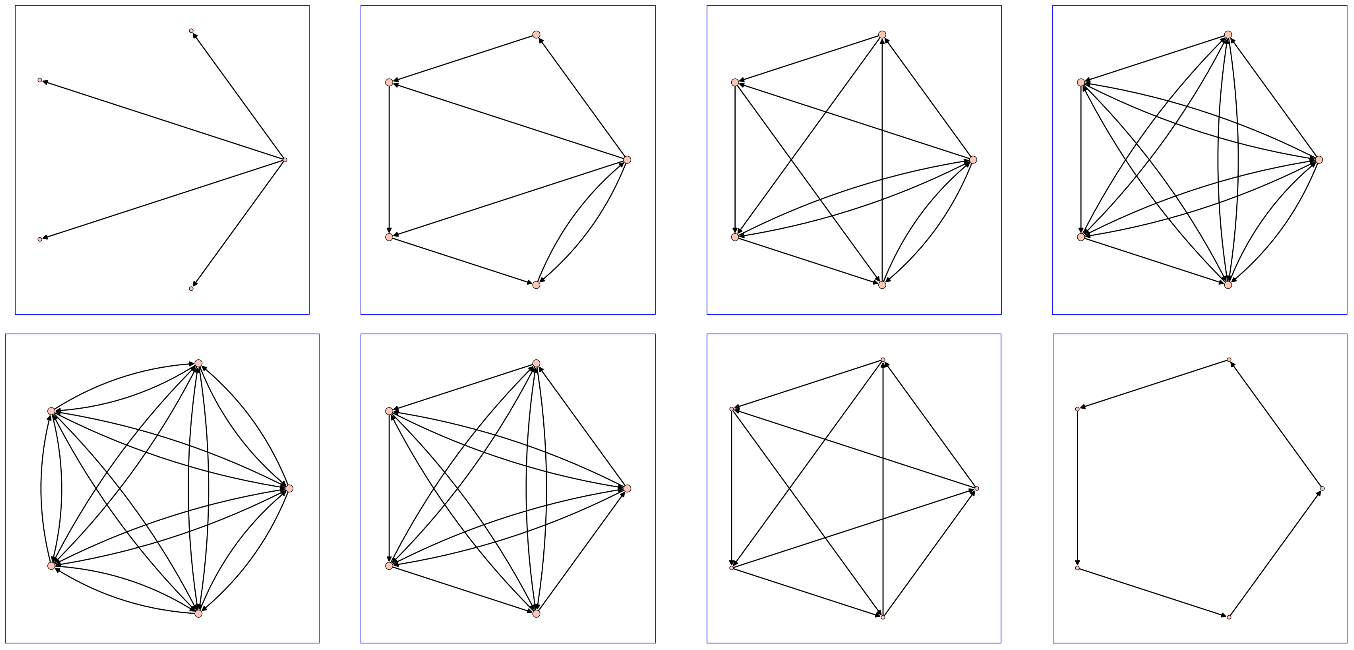
\includegraphics[width=0.95\linewidth]{figures/star2complete2path_n5.png}\\
\begin{center}
{\scalebox{1.1}{
\begin{tabular}{cccc}
~&~&~&~\\
{\scalebox{0.4}{
 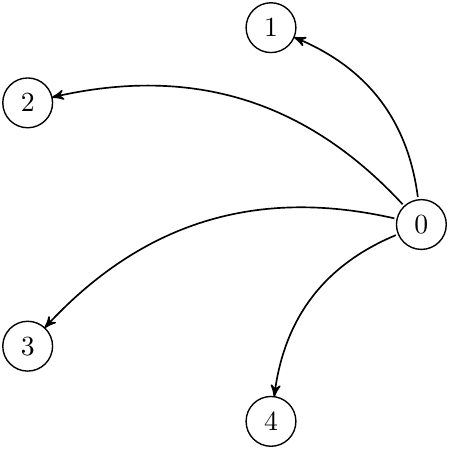
\begin{tikzpicture}
%
\useasboundingbox (0,0) rectangle (5.0cm,5.0cm);
%
\definecolor{cv0}{rgb}{0.0,0.0,0.0}
\definecolor{cfv0}{rgb}{1.0,1.0,1.0}
\definecolor{clv0}{rgb}{0.0,0.0,0.0}
\definecolor{cv1}{rgb}{0.0,0.0,0.0}
\definecolor{cfv1}{rgb}{1.0,1.0,1.0}
\definecolor{clv1}{rgb}{0.0,0.0,0.0}
\definecolor{cv2}{rgb}{0.0,0.0,0.0}
\definecolor{cfv2}{rgb}{1.0,1.0,1.0}
\definecolor{clv2}{rgb}{0.0,0.0,0.0}
\definecolor{cv3}{rgb}{0.0,0.0,0.0}
\definecolor{cfv3}{rgb}{1.0,1.0,1.0}
\definecolor{clv3}{rgb}{0.0,0.0,0.0}
\definecolor{cv4}{rgb}{0.0,0.0,0.0}
\definecolor{cfv4}{rgb}{1.0,1.0,1.0}
\definecolor{clv4}{rgb}{0.0,0.0,0.0}
\definecolor{cv0v1}{rgb}{0.0,0.0,0.0}
\definecolor{cv0v2}{rgb}{0.0,0.0,0.0}
\definecolor{cv0v3}{rgb}{0.0,0.0,0.0}
\definecolor{cv0v4}{rgb}{0.0,0.0,0.0}
%
\Vertex[style={minimum size=1.0cm,draw=cv0,fill=cfv0,text=clv0,shape=circle},LabelOut=false,L=\hbox{$0$},x=5.0cm,y=2.5cm]{v0}
\Vertex[style={minimum size=1.0cm,draw=cv1,fill=cfv1,text=clv1,shape=circle},LabelOut=false,L=\hbox{$1$},x=3.0902cm,y=5.0cm]{v1}
\Vertex[style={minimum size=1.0cm,draw=cv2,fill=cfv2,text=clv2,shape=circle},LabelOut=false,L=\hbox{$2$},x=0.0cm,y=4.0451cm]{v2}
\Vertex[style={minimum size=1.0cm,draw=cv3,fill=cfv3,text=clv3,shape=circle},LabelOut=false,L=\hbox{$3$},x=0.0cm,y=0.9549cm]{v3}
\Vertex[style={minimum size=1.0cm,draw=cv4,fill=cfv4,text=clv4,shape=circle},LabelOut=false,L=\hbox{$4$},x=3.0902cm,y=0.0cm]{v4}
%
\Edge[lw=0.1cm,style={post, bend right,color=cv0v1,},](v0)(v1)
\Edge[lw=0.1cm,style={post, bend right,color=cv0v2,},](v0)(v2)
\Edge[lw=0.1cm,style={post, bend right,color=cv0v3,},](v0)(v3)
\Edge[lw=0.1cm,style={post, bend right,color=cv0v4,},](v0)(v4)
%
\end{tikzpicture} 
}} &
 {\scalebox{0.4}{
 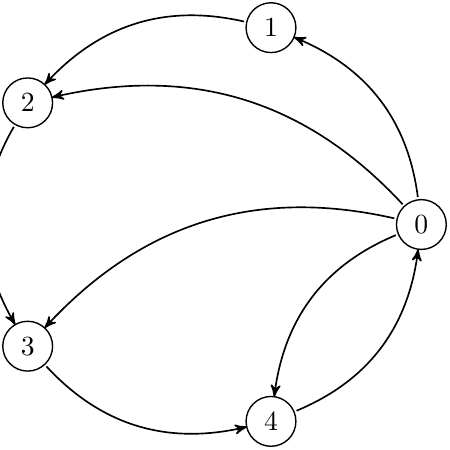
\begin{tikzpicture}
%
\useasboundingbox (0,0) rectangle (5.0cm,5.0cm);
%
\definecolor{cv0}{rgb}{0.0,0.0,0.0}
\definecolor{cfv0}{rgb}{1.0,1.0,1.0}
\definecolor{clv0}{rgb}{0.0,0.0,0.0}
\definecolor{cv1}{rgb}{0.0,0.0,0.0}
\definecolor{cfv1}{rgb}{1.0,1.0,1.0}
\definecolor{clv1}{rgb}{0.0,0.0,0.0}
\definecolor{cv2}{rgb}{0.0,0.0,0.0}
\definecolor{cfv2}{rgb}{1.0,1.0,1.0}
\definecolor{clv2}{rgb}{0.0,0.0,0.0}
\definecolor{cv3}{rgb}{0.0,0.0,0.0}
\definecolor{cfv3}{rgb}{1.0,1.0,1.0}
\definecolor{clv3}{rgb}{0.0,0.0,0.0}
\definecolor{cv4}{rgb}{0.0,0.0,0.0}
\definecolor{cfv4}{rgb}{1.0,1.0,1.0}
\definecolor{clv4}{rgb}{0.0,0.0,0.0}
\definecolor{cv0v1}{rgb}{0.0,0.0,0.0}
\definecolor{cv0v2}{rgb}{0.0,0.0,0.0}
\definecolor{cv0v3}{rgb}{0.0,0.0,0.0}
\definecolor{cv0v4}{rgb}{0.0,0.0,0.0}
\definecolor{cv1v2}{rgb}{0.0,0.0,0.0}
\definecolor{cv2v3}{rgb}{0.0,0.0,0.0}
\definecolor{cv3v4}{rgb}{0.0,0.0,0.0}
\definecolor{cv4v0}{rgb}{0.0,0.0,0.0}
%
\Vertex[style={minimum size=1.0cm,draw=cv0,fill=cfv0,text=clv0,shape=circle},LabelOut=false,L=\hbox{$0$},x=5.0cm,y=2.5cm]{v0}
\Vertex[style={minimum size=1.0cm,draw=cv1,fill=cfv1,text=clv1,shape=circle},LabelOut=false,L=\hbox{$1$},x=3.0902cm,y=5.0cm]{v1}
\Vertex[style={minimum size=1.0cm,draw=cv2,fill=cfv2,text=clv2,shape=circle},LabelOut=false,L=\hbox{$2$},x=0.0cm,y=4.0451cm]{v2}
\Vertex[style={minimum size=1.0cm,draw=cv3,fill=cfv3,text=clv3,shape=circle},LabelOut=false,L=\hbox{$3$},x=0.0cm,y=0.9549cm]{v3}
\Vertex[style={minimum size=1.0cm,draw=cv4,fill=cfv4,text=clv4,shape=circle},LabelOut=false,L=\hbox{$4$},x=3.0902cm,y=0.0cm]{v4}
%
\Edge[lw=0.1cm,style={post, bend right,color=cv0v1,},](v0)(v1)
\Edge[lw=0.1cm,style={post, bend right,color=cv0v2,},](v0)(v2)
\Edge[lw=0.1cm,style={post, bend right,color=cv0v3,},](v0)(v3)
\Edge[lw=0.1cm,style={post, bend right,color=cv0v4,},](v0)(v4)
\Edge[lw=0.1cm,style={post, bend right,color=cv1v2,},](v1)(v2)
\Edge[lw=0.1cm,style={post, bend right,color=cv2v3,},](v2)(v3)
\Edge[lw=0.1cm,style={post, bend right,color=cv3v4,},](v3)(v4)
\Edge[lw=0.1cm,style={post, bend right,color=cv4v0,},](v4)(v0)
%
\end{tikzpicture} 
}} &
 {\scalebox{0.4}{
 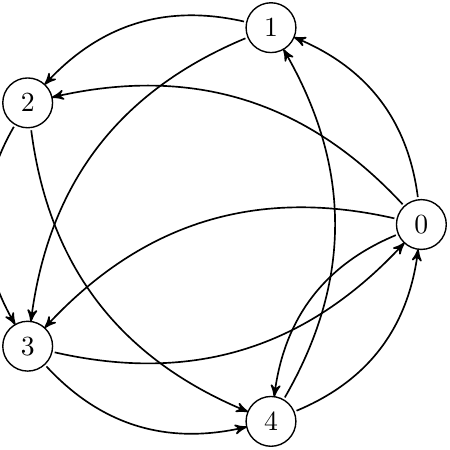
\begin{tikzpicture}
%
\useasboundingbox (0,0) rectangle (5.0cm,5.0cm);
%
\definecolor{cv0}{rgb}{0.0,0.0,0.0}
\definecolor{cfv0}{rgb}{1.0,1.0,1.0}
\definecolor{clv0}{rgb}{0.0,0.0,0.0}
\definecolor{cv1}{rgb}{0.0,0.0,0.0}
\definecolor{cfv1}{rgb}{1.0,1.0,1.0}
\definecolor{clv1}{rgb}{0.0,0.0,0.0}
\definecolor{cv2}{rgb}{0.0,0.0,0.0}
\definecolor{cfv2}{rgb}{1.0,1.0,1.0}
\definecolor{clv2}{rgb}{0.0,0.0,0.0}
\definecolor{cv3}{rgb}{0.0,0.0,0.0}
\definecolor{cfv3}{rgb}{1.0,1.0,1.0}
\definecolor{clv3}{rgb}{0.0,0.0,0.0}
\definecolor{cv4}{rgb}{0.0,0.0,0.0}
\definecolor{cfv4}{rgb}{1.0,1.0,1.0}
\definecolor{clv4}{rgb}{0.0,0.0,0.0}
\definecolor{cv0v1}{rgb}{0.0,0.0,0.0}
\definecolor{cv0v2}{rgb}{0.0,0.0,0.0}
\definecolor{cv0v3}{rgb}{0.0,0.0,0.0}
\definecolor{cv0v4}{rgb}{0.0,0.0,0.0}
\definecolor{cv1v2}{rgb}{0.0,0.0,0.0}
\definecolor{cv1v3}{rgb}{0.0,0.0,0.0}
\definecolor{cv2v3}{rgb}{0.0,0.0,0.0}
\definecolor{cv2v4}{rgb}{0.0,0.0,0.0}
\definecolor{cv3v0}{rgb}{0.0,0.0,0.0}
\definecolor{cv3v4}{rgb}{0.0,0.0,0.0}
\definecolor{cv4v0}{rgb}{0.0,0.0,0.0}
\definecolor{cv4v1}{rgb}{0.0,0.0,0.0}
%
\Vertex[style={minimum size=1.0cm,draw=cv0,fill=cfv0,text=clv0,shape=circle},LabelOut=false,L=\hbox{$0$},x=5.0cm,y=2.5cm]{v0}
\Vertex[style={minimum size=1.0cm,draw=cv1,fill=cfv1,text=clv1,shape=circle},LabelOut=false,L=\hbox{$1$},x=3.0902cm,y=5.0cm]{v1}
\Vertex[style={minimum size=1.0cm,draw=cv2,fill=cfv2,text=clv2,shape=circle},LabelOut=false,L=\hbox{$2$},x=0.0cm,y=4.0451cm]{v2}
\Vertex[style={minimum size=1.0cm,draw=cv3,fill=cfv3,text=clv3,shape=circle},LabelOut=false,L=\hbox{$3$},x=0.0cm,y=0.9549cm]{v3}
\Vertex[style={minimum size=1.0cm,draw=cv4,fill=cfv4,text=clv4,shape=circle},LabelOut=false,L=\hbox{$4$},x=3.0902cm,y=0.0cm]{v4}
%
\Edge[lw=0.1cm,style={post, bend right,color=cv0v1,},](v0)(v1)
\Edge[lw=0.1cm,style={post, bend right,color=cv0v2,},](v0)(v2)
\Edge[lw=0.1cm,style={post, bend right,color=cv0v3,},](v0)(v3)
\Edge[lw=0.1cm,style={post, bend right,color=cv0v4,},](v0)(v4)
\Edge[lw=0.1cm,style={post, bend right,color=cv1v2,},](v1)(v2)
\Edge[lw=0.1cm,style={post, bend right,color=cv1v3,},](v1)(v3)
\Edge[lw=0.1cm,style={post, bend right,color=cv2v3,},](v2)(v3)
\Edge[lw=0.1cm,style={post, bend right,color=cv2v4,},](v2)(v4)
\Edge[lw=0.1cm,style={post, bend right,color=cv3v0,},](v3)(v0)
\Edge[lw=0.1cm,style={post, bend right,color=cv3v4,},](v3)(v4)
\Edge[lw=0.1cm,style={post, bend right,color=cv4v0,},](v4)(v0)
\Edge[lw=0.1cm,style={post, bend right,color=cv4v1,},](v4)(v1)
%
\end{tikzpicture} 
}} &
 {\scalebox{0.4}{
 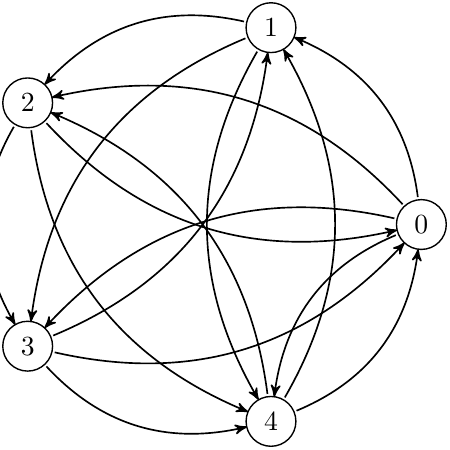
\begin{tikzpicture}
%
\useasboundingbox (0,0) rectangle (5.0cm,5.0cm);
%
\definecolor{cv0}{rgb}{0.0,0.0,0.0}
\definecolor{cfv0}{rgb}{1.0,1.0,1.0}
\definecolor{clv0}{rgb}{0.0,0.0,0.0}
\definecolor{cv1}{rgb}{0.0,0.0,0.0}
\definecolor{cfv1}{rgb}{1.0,1.0,1.0}
\definecolor{clv1}{rgb}{0.0,0.0,0.0}
\definecolor{cv2}{rgb}{0.0,0.0,0.0}
\definecolor{cfv2}{rgb}{1.0,1.0,1.0}
\definecolor{clv2}{rgb}{0.0,0.0,0.0}
\definecolor{cv3}{rgb}{0.0,0.0,0.0}
\definecolor{cfv3}{rgb}{1.0,1.0,1.0}
\definecolor{clv3}{rgb}{0.0,0.0,0.0}
\definecolor{cv4}{rgb}{0.0,0.0,0.0}
\definecolor{cfv4}{rgb}{1.0,1.0,1.0}
\definecolor{clv4}{rgb}{0.0,0.0,0.0}
\definecolor{cv0v1}{rgb}{0.0,0.0,0.0}
\definecolor{cv0v2}{rgb}{0.0,0.0,0.0}
\definecolor{cv0v3}{rgb}{0.0,0.0,0.0}
\definecolor{cv0v4}{rgb}{0.0,0.0,0.0}
\definecolor{cv1v2}{rgb}{0.0,0.0,0.0}
\definecolor{cv1v3}{rgb}{0.0,0.0,0.0}
\definecolor{cv1v4}{rgb}{0.0,0.0,0.0}
\definecolor{cv2v0}{rgb}{0.0,0.0,0.0}
\definecolor{cv2v3}{rgb}{0.0,0.0,0.0}
\definecolor{cv2v4}{rgb}{0.0,0.0,0.0}
\definecolor{cv3v0}{rgb}{0.0,0.0,0.0}
\definecolor{cv3v1}{rgb}{0.0,0.0,0.0}
\definecolor{cv3v4}{rgb}{0.0,0.0,0.0}
\definecolor{cv4v0}{rgb}{0.0,0.0,0.0}
\definecolor{cv4v1}{rgb}{0.0,0.0,0.0}
\definecolor{cv4v2}{rgb}{0.0,0.0,0.0}
%
\Vertex[style={minimum size=1.0cm,draw=cv0,fill=cfv0,text=clv0,shape=circle},LabelOut=false,L=\hbox{$0$},x=5.0cm,y=2.5cm]{v0}
\Vertex[style={minimum size=1.0cm,draw=cv1,fill=cfv1,text=clv1,shape=circle},LabelOut=false,L=\hbox{$1$},x=3.0902cm,y=5.0cm]{v1}
\Vertex[style={minimum size=1.0cm,draw=cv2,fill=cfv2,text=clv2,shape=circle},LabelOut=false,L=\hbox{$2$},x=0.0cm,y=4.0451cm]{v2}
\Vertex[style={minimum size=1.0cm,draw=cv3,fill=cfv3,text=clv3,shape=circle},LabelOut=false,L=\hbox{$3$},x=0.0cm,y=0.9549cm]{v3}
\Vertex[style={minimum size=1.0cm,draw=cv4,fill=cfv4,text=clv4,shape=circle},LabelOut=false,L=\hbox{$4$},x=3.0902cm,y=0.0cm]{v4}
%
\Edge[lw=0.1cm,style={post, bend right,color=cv0v1,},](v0)(v1)
\Edge[lw=0.1cm,style={post, bend right,color=cv0v2,},](v0)(v2)
\Edge[lw=0.1cm,style={post, bend right,color=cv0v3,},](v0)(v3)
\Edge[lw=0.1cm,style={post, bend right,color=cv0v4,},](v0)(v4)
\Edge[lw=0.1cm,style={post, bend right,color=cv1v2,},](v1)(v2)
\Edge[lw=0.1cm,style={post, bend right,color=cv1v3,},](v1)(v3)
\Edge[lw=0.1cm,style={post, bend right,color=cv1v4,},](v1)(v4)
\Edge[lw=0.1cm,style={post, bend right,color=cv2v0,},](v2)(v0)
\Edge[lw=0.1cm,style={post, bend right,color=cv2v3,},](v2)(v3)
\Edge[lw=0.1cm,style={post, bend right,color=cv2v4,},](v2)(v4)
\Edge[lw=0.1cm,style={post, bend right,color=cv3v0,},](v3)(v0)
\Edge[lw=0.1cm,style={post, bend right,color=cv3v1,},](v3)(v1)
\Edge[lw=0.1cm,style={post, bend right,color=cv3v4,},](v3)(v4)
\Edge[lw=0.1cm,style={post, bend right,color=cv4v0,},](v4)(v0)
\Edge[lw=0.1cm,style={post, bend right,color=cv4v1,},](v4)(v1)
\Edge[lw=0.1cm,style={post, bend right,color=cv4v2,},](v4)(v2)
%
\end{tikzpicture} 
}} \\ 
~&~&~&~\\
 {\scalebox{0.4}{
 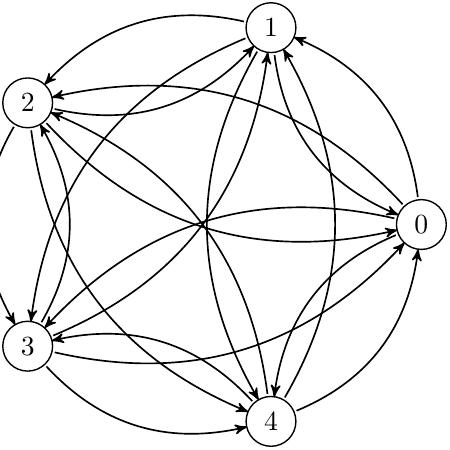
\begin{tikzpicture}
%
\useasboundingbox (0,0) rectangle (5.0cm,5.0cm);
%
\definecolor{cv0}{rgb}{0.0,0.0,0.0}
\definecolor{cfv0}{rgb}{1.0,1.0,1.0}
\definecolor{clv0}{rgb}{0.0,0.0,0.0}
\definecolor{cv1}{rgb}{0.0,0.0,0.0}
\definecolor{cfv1}{rgb}{1.0,1.0,1.0}
\definecolor{clv1}{rgb}{0.0,0.0,0.0}
\definecolor{cv2}{rgb}{0.0,0.0,0.0}
\definecolor{cfv2}{rgb}{1.0,1.0,1.0}
\definecolor{clv2}{rgb}{0.0,0.0,0.0}
\definecolor{cv3}{rgb}{0.0,0.0,0.0}
\definecolor{cfv3}{rgb}{1.0,1.0,1.0}
\definecolor{clv3}{rgb}{0.0,0.0,0.0}
\definecolor{cv4}{rgb}{0.0,0.0,0.0}
\definecolor{cfv4}{rgb}{1.0,1.0,1.0}
\definecolor{clv4}{rgb}{0.0,0.0,0.0}
\definecolor{cv0v1}{rgb}{0.0,0.0,0.0}
\definecolor{cv0v2}{rgb}{0.0,0.0,0.0}
\definecolor{cv0v3}{rgb}{0.0,0.0,0.0}
\definecolor{cv0v4}{rgb}{0.0,0.0,0.0}
\definecolor{cv1v0}{rgb}{0.0,0.0,0.0}
\definecolor{cv1v2}{rgb}{0.0,0.0,0.0}
\definecolor{cv1v3}{rgb}{0.0,0.0,0.0}
\definecolor{cv1v4}{rgb}{0.0,0.0,0.0}
\definecolor{cv2v0}{rgb}{0.0,0.0,0.0}
\definecolor{cv2v1}{rgb}{0.0,0.0,0.0}
\definecolor{cv2v3}{rgb}{0.0,0.0,0.0}
\definecolor{cv2v4}{rgb}{0.0,0.0,0.0}
\definecolor{cv3v0}{rgb}{0.0,0.0,0.0}
\definecolor{cv3v1}{rgb}{0.0,0.0,0.0}
\definecolor{cv3v2}{rgb}{0.0,0.0,0.0}
\definecolor{cv3v4}{rgb}{0.0,0.0,0.0}
\definecolor{cv4v0}{rgb}{0.0,0.0,0.0}
\definecolor{cv4v1}{rgb}{0.0,0.0,0.0}
\definecolor{cv4v2}{rgb}{0.0,0.0,0.0}
\definecolor{cv4v3}{rgb}{0.0,0.0,0.0}
%
\Vertex[style={minimum size=1.0cm,draw=cv0,fill=cfv0,text=clv0,shape=circle},LabelOut=false,L=\hbox{$0$},x=5.0cm,y=2.5cm]{v0}
\Vertex[style={minimum size=1.0cm,draw=cv1,fill=cfv1,text=clv1,shape=circle},LabelOut=false,L=\hbox{$1$},x=3.0902cm,y=5.0cm]{v1}
\Vertex[style={minimum size=1.0cm,draw=cv2,fill=cfv2,text=clv2,shape=circle},LabelOut=false,L=\hbox{$2$},x=0.0cm,y=4.0451cm]{v2}
\Vertex[style={minimum size=1.0cm,draw=cv3,fill=cfv3,text=clv3,shape=circle},LabelOut=false,L=\hbox{$3$},x=0.0cm,y=0.9549cm]{v3}
\Vertex[style={minimum size=1.0cm,draw=cv4,fill=cfv4,text=clv4,shape=circle},LabelOut=false,L=\hbox{$4$},x=3.0902cm,y=0.0cm]{v4}
%
\Edge[lw=0.1cm,style={post, bend right,color=cv0v1,},](v0)(v1)
\Edge[lw=0.1cm,style={post, bend right,color=cv0v2,},](v0)(v2)
\Edge[lw=0.1cm,style={post, bend right,color=cv0v3,},](v0)(v3)
\Edge[lw=0.1cm,style={post, bend right,color=cv0v4,},](v0)(v4)
\Edge[lw=0.1cm,style={post, bend right,color=cv1v0,},](v1)(v0)
\Edge[lw=0.1cm,style={post, bend right,color=cv1v2,},](v1)(v2)
\Edge[lw=0.1cm,style={post, bend right,color=cv1v3,},](v1)(v3)
\Edge[lw=0.1cm,style={post, bend right,color=cv1v4,},](v1)(v4)
\Edge[lw=0.1cm,style={post, bend right,color=cv2v0,},](v2)(v0)
\Edge[lw=0.1cm,style={post, bend right,color=cv2v1,},](v2)(v1)
\Edge[lw=0.1cm,style={post, bend right,color=cv2v3,},](v2)(v3)
\Edge[lw=0.1cm,style={post, bend right,color=cv2v4,},](v2)(v4)
\Edge[lw=0.1cm,style={post, bend right,color=cv3v0,},](v3)(v0)
\Edge[lw=0.1cm,style={post, bend right,color=cv3v1,},](v3)(v1)
\Edge[lw=0.1cm,style={post, bend right,color=cv3v2,},](v3)(v2)
\Edge[lw=0.1cm,style={post, bend right,color=cv3v4,},](v3)(v4)
\Edge[lw=0.1cm,style={post, bend right,color=cv4v0,},](v4)(v0)
\Edge[lw=0.1cm,style={post, bend right,color=cv4v1,},](v4)(v1)
\Edge[lw=0.1cm,style={post, bend right,color=cv4v2,},](v4)(v2)
\Edge[lw=0.1cm,style={post, bend right,color=cv4v3,},](v4)(v3)
%
\end{tikzpicture} 
}} &
 {\scalebox{0.4}{
 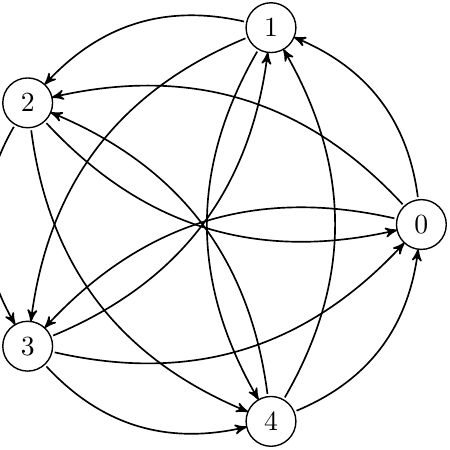
\begin{tikzpicture}
%
\useasboundingbox (0,0) rectangle (5.0cm,5.0cm);
%
\definecolor{cv0}{rgb}{0.0,0.0,0.0}
\definecolor{cfv0}{rgb}{1.0,1.0,1.0}
\definecolor{clv0}{rgb}{0.0,0.0,0.0}
\definecolor{cv1}{rgb}{0.0,0.0,0.0}
\definecolor{cfv1}{rgb}{1.0,1.0,1.0}
\definecolor{clv1}{rgb}{0.0,0.0,0.0}
\definecolor{cv2}{rgb}{0.0,0.0,0.0}
\definecolor{cfv2}{rgb}{1.0,1.0,1.0}
\definecolor{clv2}{rgb}{0.0,0.0,0.0}
\definecolor{cv3}{rgb}{0.0,0.0,0.0}
\definecolor{cfv3}{rgb}{1.0,1.0,1.0}
\definecolor{clv3}{rgb}{0.0,0.0,0.0}
\definecolor{cv4}{rgb}{0.0,0.0,0.0}
\definecolor{cfv4}{rgb}{1.0,1.0,1.0}
\definecolor{clv4}{rgb}{0.0,0.0,0.0}
\definecolor{cv0v1}{rgb}{0.0,0.0,0.0}
\definecolor{cv0v2}{rgb}{0.0,0.0,0.0}
\definecolor{cv0v3}{rgb}{0.0,0.0,0.0}
\definecolor{cv1v2}{rgb}{0.0,0.0,0.0}
\definecolor{cv1v3}{rgb}{0.0,0.0,0.0}
\definecolor{cv1v4}{rgb}{0.0,0.0,0.0}
\definecolor{cv2v0}{rgb}{0.0,0.0,0.0}
\definecolor{cv2v3}{rgb}{0.0,0.0,0.0}
\definecolor{cv2v4}{rgb}{0.0,0.0,0.0}
\definecolor{cv3v0}{rgb}{0.0,0.0,0.0}
\definecolor{cv3v1}{rgb}{0.0,0.0,0.0}
\definecolor{cv3v4}{rgb}{0.0,0.0,0.0}
\definecolor{cv4v0}{rgb}{0.0,0.0,0.0}
\definecolor{cv4v1}{rgb}{0.0,0.0,0.0}
\definecolor{cv4v2}{rgb}{0.0,0.0,0.0}
%
\Vertex[style={minimum size=1.0cm,draw=cv0,fill=cfv0,text=clv0,shape=circle},LabelOut=false,L=\hbox{$0$},x=5.0cm,y=2.5cm]{v0}
\Vertex[style={minimum size=1.0cm,draw=cv1,fill=cfv1,text=clv1,shape=circle},LabelOut=false,L=\hbox{$1$},x=3.0902cm,y=5.0cm]{v1}
\Vertex[style={minimum size=1.0cm,draw=cv2,fill=cfv2,text=clv2,shape=circle},LabelOut=false,L=\hbox{$2$},x=0.0cm,y=4.0451cm]{v2}
\Vertex[style={minimum size=1.0cm,draw=cv3,fill=cfv3,text=clv3,shape=circle},LabelOut=false,L=\hbox{$3$},x=0.0cm,y=0.9549cm]{v3}
\Vertex[style={minimum size=1.0cm,draw=cv4,fill=cfv4,text=clv4,shape=circle},LabelOut=false,L=\hbox{$4$},x=3.0902cm,y=0.0cm]{v4}
%
\Edge[lw=0.1cm,style={post, bend right,color=cv0v1,},](v0)(v1)
\Edge[lw=0.1cm,style={post, bend right,color=cv0v2,},](v0)(v2)
\Edge[lw=0.1cm,style={post, bend right,color=cv0v3,},](v0)(v3)
\Edge[lw=0.1cm,style={post, bend right,color=cv1v2,},](v1)(v2)
\Edge[lw=0.1cm,style={post, bend right,color=cv1v3,},](v1)(v3)
\Edge[lw=0.1cm,style={post, bend right,color=cv1v4,},](v1)(v4)
\Edge[lw=0.1cm,style={post, bend right,color=cv2v0,},](v2)(v0)
\Edge[lw=0.1cm,style={post, bend right,color=cv2v3,},](v2)(v3)
\Edge[lw=0.1cm,style={post, bend right,color=cv2v4,},](v2)(v4)
\Edge[lw=0.1cm,style={post, bend right,color=cv3v0,},](v3)(v0)
\Edge[lw=0.1cm,style={post, bend right,color=cv3v1,},](v3)(v1)
\Edge[lw=0.1cm,style={post, bend right,color=cv3v4,},](v3)(v4)
\Edge[lw=0.1cm,style={post, bend right,color=cv4v0,},](v4)(v0)
\Edge[lw=0.1cm,style={post, bend right,color=cv4v1,},](v4)(v1)
\Edge[lw=0.1cm,style={post, bend right,color=cv4v2,},](v4)(v2)
%
\end{tikzpicture} 
}} &
 {\scalebox{0.4}{
 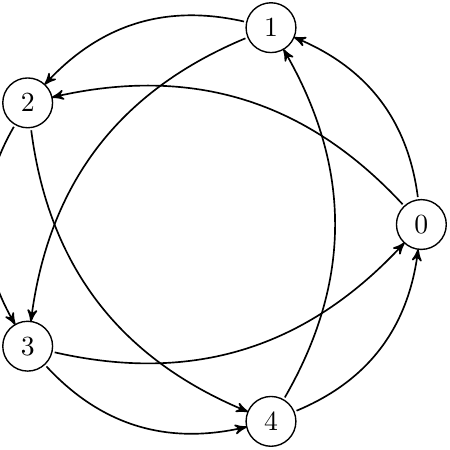
\begin{tikzpicture}
%
\useasboundingbox (0,0) rectangle (5.0cm,5.0cm);
%
\definecolor{cv0}{rgb}{0.0,0.0,0.0}
\definecolor{cfv0}{rgb}{1.0,1.0,1.0}
\definecolor{clv0}{rgb}{0.0,0.0,0.0}
\definecolor{cv1}{rgb}{0.0,0.0,0.0}
\definecolor{cfv1}{rgb}{1.0,1.0,1.0}
\definecolor{clv1}{rgb}{0.0,0.0,0.0}
\definecolor{cv2}{rgb}{0.0,0.0,0.0}
\definecolor{cfv2}{rgb}{1.0,1.0,1.0}
\definecolor{clv2}{rgb}{0.0,0.0,0.0}
\definecolor{cv3}{rgb}{0.0,0.0,0.0}
\definecolor{cfv3}{rgb}{1.0,1.0,1.0}
\definecolor{clv3}{rgb}{0.0,0.0,0.0}
\definecolor{cv4}{rgb}{0.0,0.0,0.0}
\definecolor{cfv4}{rgb}{1.0,1.0,1.0}
\definecolor{clv4}{rgb}{0.0,0.0,0.0}
\definecolor{cv0v1}{rgb}{0.0,0.0,0.0}
\definecolor{cv0v2}{rgb}{0.0,0.0,0.0}
\definecolor{cv1v2}{rgb}{0.0,0.0,0.0}
\definecolor{cv1v3}{rgb}{0.0,0.0,0.0}
\definecolor{cv2v3}{rgb}{0.0,0.0,0.0}
\definecolor{cv2v4}{rgb}{0.0,0.0,0.0}
\definecolor{cv3v0}{rgb}{0.0,0.0,0.0}
\definecolor{cv3v4}{rgb}{0.0,0.0,0.0}
\definecolor{cv4v0}{rgb}{0.0,0.0,0.0}
\definecolor{cv4v1}{rgb}{0.0,0.0,0.0}
%
\Vertex[style={minimum size=1.0cm,draw=cv0,fill=cfv0,text=clv0,shape=circle},LabelOut=false,L=\hbox{$0$},x=5.0cm,y=2.5cm]{v0}
\Vertex[style={minimum size=1.0cm,draw=cv1,fill=cfv1,text=clv1,shape=circle},LabelOut=false,L=\hbox{$1$},x=3.0902cm,y=5.0cm]{v1}
\Vertex[style={minimum size=1.0cm,draw=cv2,fill=cfv2,text=clv2,shape=circle},LabelOut=false,L=\hbox{$2$},x=0.0cm,y=4.0451cm]{v2}
\Vertex[style={minimum size=1.0cm,draw=cv3,fill=cfv3,text=clv3,shape=circle},LabelOut=false,L=\hbox{$3$},x=0.0cm,y=0.9549cm]{v3}
\Vertex[style={minimum size=1.0cm,draw=cv4,fill=cfv4,text=clv4,shape=circle},LabelOut=false,L=\hbox{$4$},x=3.0902cm,y=0.0cm]{v4}
%
\Edge[lw=0.1cm,style={post, bend right,color=cv0v1,},](v0)(v1)
\Edge[lw=0.1cm,style={post, bend right,color=cv0v2,},](v0)(v2)
\Edge[lw=0.1cm,style={post, bend right,color=cv1v2,},](v1)(v2)
\Edge[lw=0.1cm,style={post, bend right,color=cv1v3,},](v1)(v3)
\Edge[lw=0.1cm,style={post, bend right,color=cv2v3,},](v2)(v3)
\Edge[lw=0.1cm,style={post, bend right,color=cv2v4,},](v2)(v4)
\Edge[lw=0.1cm,style={post, bend right,color=cv3v0,},](v3)(v0)
\Edge[lw=0.1cm,style={post, bend right,color=cv3v4,},](v3)(v4)
\Edge[lw=0.1cm,style={post, bend right,color=cv4v0,},](v4)(v0)
\Edge[lw=0.1cm,style={post, bend right,color=cv4v1,},](v4)(v1)
%
\end{tikzpicture} 
}} &
 {\scalebox{0.4}{
 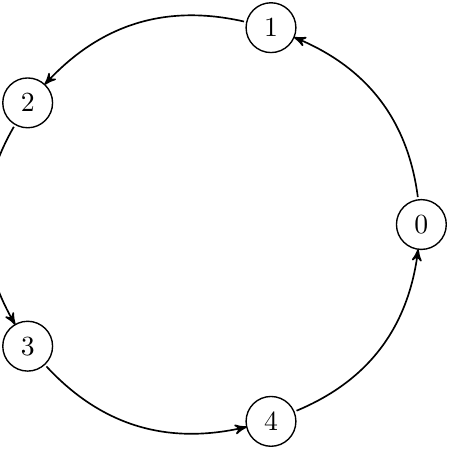
\begin{tikzpicture}
%
\useasboundingbox (0,0) rectangle (5.0cm,5.0cm);
%
\definecolor{cv0}{rgb}{0.0,0.0,0.0}
\definecolor{cfv0}{rgb}{1.0,1.0,1.0}
\definecolor{clv0}{rgb}{0.0,0.0,0.0}
\definecolor{cv1}{rgb}{0.0,0.0,0.0}
\definecolor{cfv1}{rgb}{1.0,1.0,1.0}
\definecolor{clv1}{rgb}{0.0,0.0,0.0}
\definecolor{cv2}{rgb}{0.0,0.0,0.0}
\definecolor{cfv2}{rgb}{1.0,1.0,1.0}
\definecolor{clv2}{rgb}{0.0,0.0,0.0}
\definecolor{cv3}{rgb}{0.0,0.0,0.0}
\definecolor{cfv3}{rgb}{1.0,1.0,1.0}
\definecolor{clv3}{rgb}{0.0,0.0,0.0}
\definecolor{cv4}{rgb}{0.0,0.0,0.0}
\definecolor{cfv4}{rgb}{1.0,1.0,1.0}
\definecolor{clv4}{rgb}{0.0,0.0,0.0}
\definecolor{cv0v1}{rgb}{0.0,0.0,0.0}
\definecolor{cv1v2}{rgb}{0.0,0.0,0.0}
\definecolor{cv2v3}{rgb}{0.0,0.0,0.0}
\definecolor{cv3v4}{rgb}{0.0,0.0,0.0}
\definecolor{cv4v0}{rgb}{0.0,0.0,0.0}
%
\Vertex[style={minimum size=1.0cm,draw=cv0,fill=cfv0,text=clv0,shape=circle},LabelOut=false,L=\hbox{$0$},x=5.0cm,y=2.5cm]{v0}
\Vertex[style={minimum size=1.0cm,draw=cv1,fill=cfv1,text=clv1,shape=circle},LabelOut=false,L=\hbox{$1$},x=3.0902cm,y=5.0cm]{v1}
\Vertex[style={minimum size=1.0cm,draw=cv2,fill=cfv2,text=clv2,shape=circle},LabelOut=false,L=\hbox{$2$},x=0.0cm,y=4.0451cm]{v2}
\Vertex[style={minimum size=1.0cm,draw=cv3,fill=cfv3,text=clv3,shape=circle},LabelOut=false,L=\hbox{$3$},x=0.0cm,y=0.9549cm]{v3}
\Vertex[style={minimum size=1.0cm,draw=cv4,fill=cfv4,text=clv4,shape=circle},LabelOut=false,L=\hbox{$4$},x=3.0902cm,y=0.0cm]{v4}
%
\Edge[lw=0.1cm,style={post, bend right,color=cv0v1,},](v0)(v1)
\Edge[lw=0.1cm,style={post, bend right,color=cv1v2,},](v1)(v2)
\Edge[lw=0.1cm,style={post, bend right,color=cv2v3,},](v2)(v3)
\Edge[lw=0.1cm,style={post, bend right,color=cv3v4,},](v3)(v4)
\Edge[lw=0.1cm,style={post, bend right,color=cv4v0,},](v4)(v0)
%
\end{tikzpicture} 
}}
 \end{tabular}

}}
\end{center}
\caption{A path from star network to circular path network through the complete network with 5 vertices (in z-pattern layout).\label{F:star2complete2path_n5}}
\end{figure}

We can finally see in \autoref{F:MLE_AandB_star2complete2path_n50_reps10_last} how the probability density function (PDF) of the MLEs, $(\widehat{\alpha},\widehat{\beta})$, change as we sequentially vary the SICN in the family that interpolates from the star network (red hue) to the circular path network (pink hue) via the complete network (blue hue).  
The MLEs is based on $10$ independent transmission trees simulated from each SICN in the sequence of $98$ SICNs over a population of size $n=50$.  
In \autoref{F:MLE_AandB_star2complete2path_n50_reps10_last}, the hue of the PDFs sequentially change from red which is concentrated entirely on the boundary at $1$ (star network), to orange and yellow which are decreasing their concentration at $1$ due to disappearance of the star's signal from the larger neighbourhoods of the circulant graphs $\mathsf{C}(n,\mathbb{A}_i)$.  
As $i$ approaches $n-1$ the green and azure hues of the PDFs become increasingly uniform around blue when the SICN is the complete network.  
The hue of the PDFs become purple and start concentrating at $0$ as the SICN approaches the path network that is fully concentrated at $0$ (pink hue). 
The pattern of the PDFs is stochastic since it is based on MLEs from just 10 samples.  
However, it clearly demonstrates that the interpolating sequence in the space of SICNs does convey continuity in the parameter space of $(\alpha,\beta)$.
In other words, this suggests that there is an $(\alpha,\beta)$ under the Beta-splitting model (recall that the Beta-splitting model need not explicitly refer to the contact network), that best fits the distribution of transmission trees generated from any specific contact network.  


\begin{figure}[htbp]
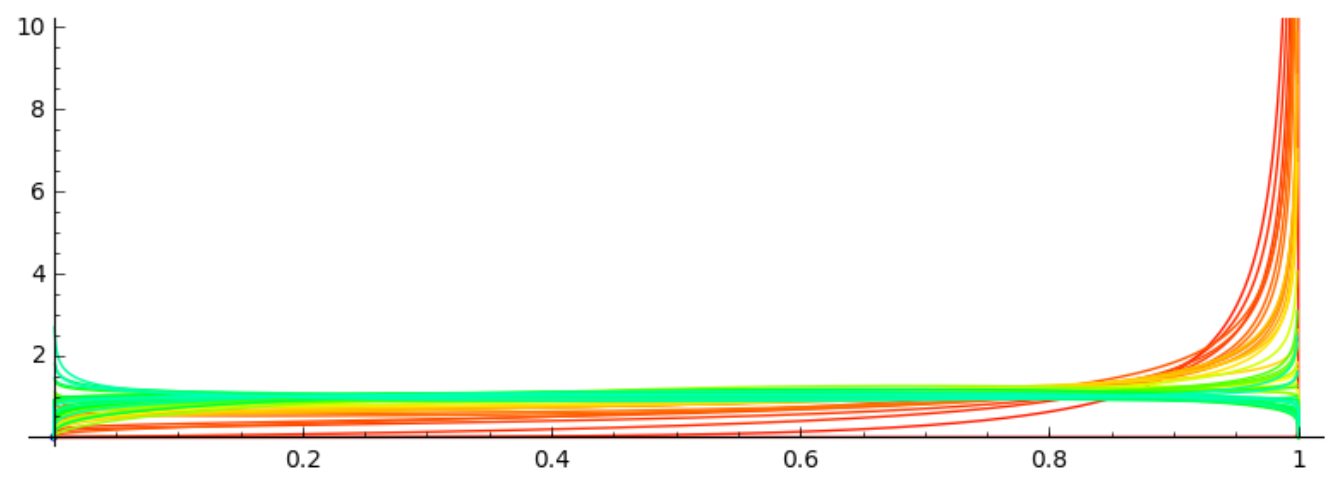
\includegraphics[width=0.95\linewidth]{figures/MLE_AandB_star2complete2path_n50_reps10_first.png}\\
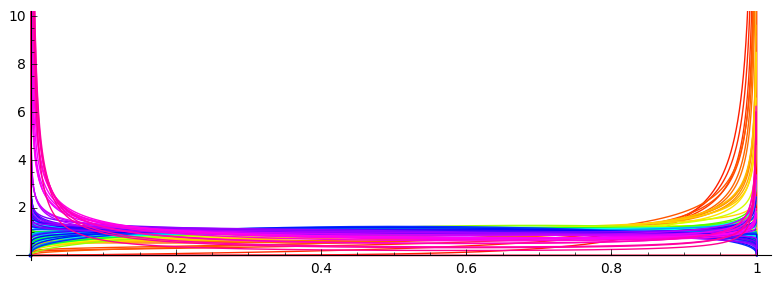
\includegraphics[width=0.95\linewidth]{figures/MLE_AandB_star2complete2path_n50_reps10_last.png}
\caption{Probability density function (PDF) of the $\mathcal{B}(\alpha+1,\beta+1)$ distribution at the maximum likelihood estimates of $\alpha$ and $\beta$ based on $10$ sampled transmission trees from each SICN in the sequential family that interpolates from the star network (red hue) to the circular path network (pink hue) via the complete network (blue hue) with $n=50$ vertices. The hue of the PDFs sequentially change from red (star network), orange, yellow and green (complete network) as shown on the top plot and continue on with azure, blue, purple, to pink (path network) as shown in the bottom plot.\label{F:MLE_AandB_star2complete2path_n50_reps10_last}}
\end{figure}


The sufficient statistics of split-pair frequencies for $\alpha$ and $\beta$ from various stages of the interpolating family of SICNs spanning the star, complete and path network are shown in \autoref{F:SuffStatsStar2Complete2Path_n100_r1001}.  
Note how these sufficient statistics are also changing gradually as expected.

\begin{figure}[htbp]
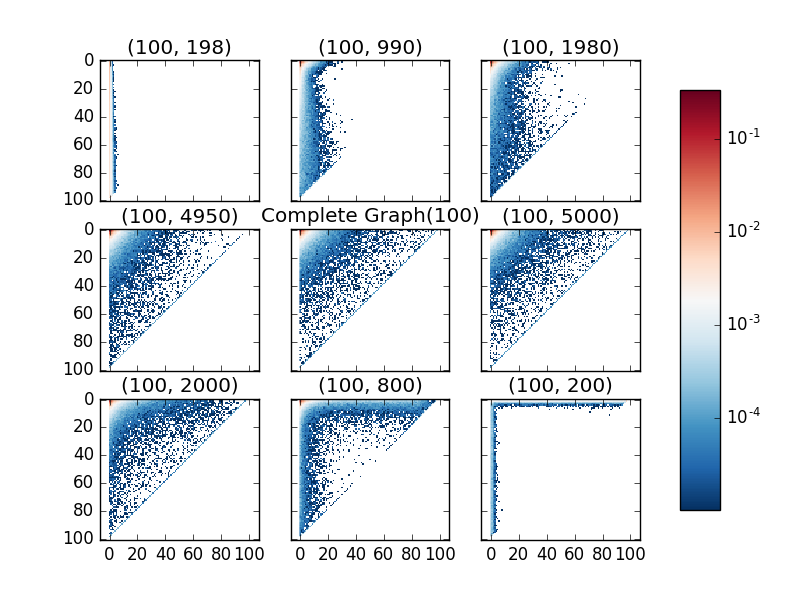
\includegraphics[width=0.95\linewidth]{figures/SuffStatsStar2Complete2Path_n100_r1001.png}\\
\caption{The sufficient statistics of split-pair frequencies for $\alpha$ and $\beta$ shown as the empirical mass function from 1000 independent transmission trees over a population of size $n=100$ at various stages of the interpolating family spanning the star, complete (in the center of the panel with 100 vertices and 9900 edges) and path networks (the sub-plots are labelled by the number of vertices and edges in the host contact network).\label{F:SuffStatsStar2Complete2Path_n100_r1001}}
\end{figure}

\subsection{Implications for statistical inference}\label{S:ImplicationsForStatisticalInference}

We have deliberately confined the inferential aspects of this study to the classical maximum likelihood estimator in the simplest sampling setting involving fully grown transmission trees with $n$ leaves over $r$ independent trials.  
This merely amounts to inferring the underlying contact network via multiple random breadth-first expansions that are encoded through rooted, ranked, planar, labelled, and binary (spanning) trees, i.e.~our transmission trees.  
We now give some basic insights into two other natural approaches to inference for applied network scientists and also provide some natural extensions of the likelihood function.

\subsubsection{An $L_1$ perspective}\label{S:AnL1Perspective}
We could have also defined the effective Beta-splitting model by minimizing the total variation distance between $\Pr((s^L,s^R);[c(0)])$, the probabilities on $\mathcal{S}_n$ generated by the transmission process unfolding on the product space of transmission trees and SICNs with initial SICNs in $[c(0)]$, and $\Pr((s^L,s^R); \alpha,\beta)$, the probabilities generated by the Beta-splitting model as follows:
\begin{equation}\label{E:TVrule}
(\alpha^*,\beta^*) := \argmin_{(\alpha,\beta) \in (-1,\infty)^2} \quad
\frac{1}{2} \, \sum_{(s^L,s^R) \in \mathcal{S}_n} \left| \Pr((s^L,s^R);[c(0)]) - \Pr((s^L,s^R); \alpha,\beta) \right| \enspace.
\end{equation}
One elegant aspect of this $L_1$-minimizing rule, as opposed to the likelihood maximizing rule behind MLE, is its desirable non-parametric decision-theoretic properties, such as being a metric on all probability distributions over $\mathcal{S}_n$, having easily interpretable distances in the universal scale of $[0,1]$, and having well-known relations to other statistical notions of divergence.  
For these reasons we believe that the $L_1$-minimizing rule, if efficiently implementable, would lead to better statistical properties for the task of characterizing the equivalence class based on empirical $\hat{P}$ of relative frequencies on $\mathcal{S}_n$ as opposed to the exact $\Pr((s^L,s^R); [c(0)])$ in \autoref{E:TVrule}.  

Unfortunately, an efficient numerical procedure for the minimization problem above is not yet available as it would require expressions 
for $\{\Pr((s^L,s^R); \alpha,\beta)\}$ as a function of $(\alpha,\beta) \in (-1,\infty)^2$ analogous to the loglikelihood expressions.
Such efficient expressions require further transformation of the probabilities at the rooted unranked planar and leaf-unlabelled resolution of transmission trees \cite[Lemma 4.1]{SainudiinVeber2016} onto $\mathcal{S}_n$, which is nothing but the planar unordered cousin of Aldous' shape statistics sequence \citep[Eqn.~(4.1)]{SainudiinStadlerVeber2015}.  
Note that  Aldous' shape statistics sequence, even in its original non-planar form \citep{Aldous2001}, can itself be further projected to various tree shape statistics \cite[p.~1231]{SainudiinStadlerVeber2015} used routinely in simulation-based studies of transmission trees sketched earlier in \autoref{sec:intro}. 

\subsubsection{A Bayesian perspective}
We saw that the $L_1$ perspective has some merits, provided appropriate expressions can be obtained.  
In defense of the likelihood principle on the other hand, the exact likelihood expressions developed here are most useful to Bayesian methods of inference that further incorporate prior information with the likelihood function based on finite samples.  
For example, if we know that the underlying contact network is complete then we can invoke appropriate parametric families of prior distributions centred at $(0,0)$, the known MLE for the complete network, with variance in priors reflecting our extent of this prior knowledge.  
Using the simulation-based approach of \autoref{S:ClassicalSICNFamilies} we can obtain 
the effective Beta-splitting model parameters with standard errors that can inform the formulation of appropriate prior distributions.  
Such a prior formulation can not only reflect the sample sizes, number of leaves in possibly partially observed transmission trees, etc.~at our disposal, but also various aspects of the contact networks from other sources of information such as 
(i) transportation networks and cell-signal triangulated or GPS-based location networks, etc.~that underpin coarse structural information of the host contact process in the context of a communicable disease or (ii) Twitter follower networks in the context of ``cultural'' transmission events that are defined merely to be retweets or mentions, for example (see \autoref{S:D_TowardsCulturalTransmissions}).  

Thus, inducing priors over the parameter space $[-1,\infty)^2$ for more complex analytically intractable models through their effective Beta-splitting models will now be possible, due to our efficient likelihood expressions, using current semi-parametric and variational Bayes methods, including the composition of different effective Beta-splitting models as finite mixtures with possibly unknown number of components over different sub-network neighbourhoods covering the entire contact network. 

\subsubsection{Natural extensions of the likelihood function}\label{S:NaturalExtensionsOfTheLikelihoodFunction}

Next we provide some natural extensions of the likelihood expressions developed here.
%TODO
%% needs editing for incormporation - from p.24"
%To focus on the jump chain's discrete structural information about the combinatorial skeletons of the contact network buried within the distribution over discrete transmission trees, as a necessary prelude to \autoref{T:effectiveBetaSplitting},
%our likelihood expressions in \autorefs{E:perNodeMLE}, \ref{E:lkl0},\ref{E:lkl1} and \ref{E:lkl2} are {\em skeletal} and ignore leaf labels and the waiting times between events (see code in \autoref{Sec:codeC}).
%However, the likelihood function can be easily extended as remarked in \autoref{S:NaturalExtensionsOfTheLikelihoodFunction}.
%%%%%%%%%%%%%%%%%%%%%%%%%%%%%%%%%%%%%%%%%%%%%%%
\begin{remark}\label{R:ElaborateLklFuncs1}
The likelihood function can be extended to include branch-lengths -- especially under the independent but possibly non-identical exponential waiting-times assumption in the generator of the encompassing continuous time Markov chain given by \autoref{E:GenCTchainProb}, as is the case for the complete, star and path networks studied here.  
Leaf labels can also be added according to a tractable labelling process of the population as per \autoref{E:ProbOfTTLeafLabels}.
\end{remark}

\begin{remark}\label{R:ElaborateLklFuncs2}
More crucially, the likelihood expressions naturally generalize to transmission trees that are only partially grown or in the process of growing at the time of observation so that they have fewer than $n$ leaves encoding all currently infected individuals.  
For such {\em partial likelihood} expressions one merely needs to specify $\mathcal{I}(\tau_i)$, the set of internal vertices in the $i$-th partially grown transmission tree $\tau_i$, in \autoref{E:lkl0} and let this specification imply to its consequent expressions. 
Also note that the second product over internal vertices within tree $\tau_i$ in \autoref{E:lkl0} allows each $\mathcal{I}(\tau_i)$ to be distinct with its own size, i.e., $|\mathcal{I}(\tau_i)| \in \{1,2,\ldots,n-1\}$. 
Such natural extensions of the likelihood expressions may be necessary in applied contexts and do produce maximum likelihood estimates with larger standard errors at least in some cases (results not shown here).  
However, their asymptotic consistency is expected to depend on the details of the SICN itself and on how often one samples trees with nearly $n$ leaves and/or on the initialization mechanisms for the first infector across the $r$ independently drawn partial trees.  
These partial likelihoods are implementable by modifying the lists being comprehended over vertices in \autoref{Sec:codeA} and/or \autoref{Sec:codeC}, for instance.  
\end{remark}

In this work, for concreteness and clarity, we keep the transmission trees full with $n$ leaves representing the final state when the infection has invaded the whole population.  
Due to this assumption, the {\em unordered} split-fair frequencies in \autoref{E:SuffStats} become sufficient for $\alpha$ and $\beta$.  
When allowing for multiple but independent partial trees of possibly different sizes less than $n$ as per \autoref{R:ElaborateLklFuncs2}, the unordered split-fair frequencies will still remain sufficient, provided the sampling strategy is asymptotically consistent for the underlying initial SICN, albeit one may only be observing split-pair frequencies over a subset of $\mathcal{S}_n$.  

The sufficiency of unordered split-fair frequencies over $\mathcal{S}_n$ may no longer hold for (i) more complex extensions of the likelihood which may involve non-static or temporally varying networks or for (ii) multiple simultaneous partial transmission trees grown on the same static network up to possibly random discrete stopping time $M$ from a set of initially infected vertices (especially when the set of their infected vertices become mutually incident before time $M$).  
Simplest extensions of the Beta-splitting model via finite mixtures for instance could be constructed to approximate such more realistic models by limiting oneself to the sufficient statistics of {\em ordered split-pair frequencies}:
\begin{equation}\label{E:OrderedSplitPairFrequencies}
\{ f(s^L,s^R,z) : (s^L,s^R,z) \in \mathcal{S}_n \times \{0,1,2\ldots,M\} \} \enspace,
\end{equation}
where $z$ is the discrete time index, and over products of such ordered split-pair frequencies.  
We could allow $z$ to belong to $\mathbb{Z}_0$ and even allow $n \to \infty$ in order to study contact networks in the large population limit with or without appropriate rescaling of discrete time into the continuum, for the purposes of ignoring combinatorial complications of the modelled {\em individuals} in such limits, where possible and sensible.

\section{Discussion}\label{S:Discussion}

We give a probabilistic description of the transmission process in \autoref{S:Model} as a Markov chain on the product space of SI-tagged contact networks (SICNs) and transmission trees in discrete and continuous time.  
The Markov chain is also constructed as a randomized algorithm in the SageMath/Python code in \autoref{Sec:codeA}.  
This formalizes a large class of simulation programs in the computational epidemiology literature as a transmission process.  
The probabilities of transmission trees as an explicit function of both branch-lengths and tree topologies are derived in \autoref{S:Examples} from the general Markov chains of \autorefs{E:GenJumpchainProb} and \ref{E:GenCTchainProb} for some simple static contact networks.  

Although the Markov chain model is general and only needs a directed weighted graph, our examples were limited to simple connected networks with each weight set to $1$ in order to focus on the combinatorial skeletons of their associated topological Markov chains.  
It is relatively straightforward to consider the dynamics on more general networks using the richer language for digraphs \citep[Fig.~4]{pastor2015}.  
For example, the epidemic will spread to the strongly connected giant component (if it exists) and the giant out-component, provided the infection starts from one of the vertices in either the strongly connected giant component or in a giant in-component. 

We then develop a biparametric Beta-splitting family of models for the growth of transmission trees in \autoref{S:BetaSplit} that gives the exact probability of any transmission tree as a function of $\alpha > -1$ and $\beta> -1$.  
The model can be interpreted in terms of a Beta-splitting construction for the ``infection potential'' of the infector and the infectee.
Thus, the model captures aspects of the underlying contact network up to how its contact structure affects the infection potential of the infector and infectee after the infection event.
The approach avoids the explicit modeling of the underlying contact network (that is typically unobserved or only partially observed) in order to grow transmission trees, unlike the general Markov chain models of \autorefs{E:GenJumpchainProb} and \ref{E:GenCTchainProb}.  
The Beta-splitting family of models is shown analytically to contain the models generated by the complete network ($k_n$) when $(\alpha,\beta)$ equals $(0,0)$, star network ($\star_n$) when $(\alpha,\beta) \rightarrow (\infty,-1)$ and path network ($p_n$)  when $(\alpha,\beta) \rightarrow (-1,\infty)$.  
We also derive explicit expressions for the maximum likelihood estimator and sufficient statistics of split-pair frequencies for the Beta-splitting model from independent observations of the transmission trees.  
Using the distributions on split-pairs we specify equivalence classes of initial SICNs that are indistinguishable by their Beta-splitting transmission trees with the same effective Beta-splitting model through their Beta-projections into the quarter-plane $(-1,\infty)^2$ as conjectured in \citep{UCDMS20154}.  
%This conjecture fro UCDMS2015/4 is proven in UCDMS2016/1
%We conjecture that there is an equivalence class of SI-tagged contact networks that are indistinguishable by their transmission tree distributions for some given $(\alpha,\beta) \in (-1,\infty)^2$.  
We have also shown by simulations coupled with an inferential maximum likelihood procedure that the best-fitting parameters of the effective Beta-splitting models based on samples of trees grown over (i) six deterministic contact networks and four random contact networks seem to be well-separated under their Beta-projections into $(-1,\infty)^2$ and (ii) the Beta-projections of a sequential family of SI-tagged contact networks from $\star_n$ to $k_n$ to $p_n$ do indeed change gradually in $(-1,\infty)^2$ from $(\infty,-1)$ to $(0,0)$ to $(-1,\infty)$.  
Various natural implications for statistical inference were outlined for future work.  
In the following sections we discuss some obstacles that need to be overcome for a few other important extensions of this work.

\subsection{Towards births and deaths}\label{S:D_TowardsBirthsAndDeaths}

Recall from \autoref{sec:intro} that our construction needs a {\em tagged contact network}.  
We only focus on the simplest binary tags (S and I) here and thus limited ourselves to SI-tagged contact networks (SICNs).  
This simple setting allowed us to obtain our main results here because of the underlying core process being one of pure birth events, whereby individuals `are born' from the set of vertices tagged by S into the set tagged by I at some rate.  
Thus, there is no `death' here, in the sense of vertices with tag I being retagged for `removal' with tag R (SIR model).  
The tag R denotes recovery from the infection (after having learnt how to fight the infection at some other rate).  
In the SIR model the R-tagged individual does not get retagged by S or I.    
One could represent such a sequence of birth and death events by a binary sequence that could be encoded by Dyck paths that satisfy natural conditions depending on the encoding for the SIR model.  
By further incorporating such Dyck paths and the three tags one could extend the Markov chains defined here and try to study the distributions they induce on trees with leaves recruited from the vertices with the tag S into vertices with tag I and those with tag I replaced by tag R (and frozen, in the sense of not having any further descendents) at different rates.  
Extensions to SIR model which allows for the `removal' of infected individuals from the population at a given rate is also conceivable via mapping to percolation on semi-directed networks (see \cite[V.B.4]{pastor2015} and the references therein).  

By considering birth and death processes, as opposed to a pure birth process, one can also make progress on developing transmission processes with only two tags for the more complex SIS epidemic model that not only allows susceptible individuals to become infected by any infected individual at a given `birth' rate but also allows infected individuals to become susceptible again according to a given `death' rate.  Such as model is interesting from a discrete dynamics viewpoint since one could allow the discrete time $z$ to continue to infinity and study time-asymptotic distributions over SIS transmission trees -- the same set of transmission trees for the Markov chains developed here, but with the number of leaf nodes being allowed to be any appropriate number in $\{0,1,\ldots,n\}$ at time $z \in \mathbb{Z}_0$, and with all leaf vertices tagged by I (as implicitly done here) with an absorbing state when the tree has $0$ leaves with no infected individual or by conditioning on specific set of Dyck paths \citep{Addario-Berry2008} that remove such absorption events.
The Markov chains for these problems will need more complicated state spaces and immediate precedence rules for state transitions that take the possibly conditioned Dyck paths into account.  
It is not clear how one could extend the Beta-splitting construction in an interpretable manner for these settings. 
 
\subsection{Towards cultural transmissions}\label{S:D_TowardsCulturalTransmissions}
%%%%%start edit
The insights developed here through the SICNs and their transmission trees are also applicable to the simplest models of ``meme'' \citep[][p.~192]{Dawkins1976} evolution in online social media networks \citep{SolonWIREDHawkinsMeme2013} through transmission events that can be distilled (admittedly naively) from observable actions such as `likes', `mentions', `retweets' and `+1s' along with any concomitant comments.  
See a dataset spotlight \citep{Rishal2016} in the official blog of Kaggle.com for a specific extremist cultural context.  
We would like to point out that the 55 models and their parameter choices were partly informed by empirical insights from extracting, transforming, loading and exploring the raw tweets available to Twitter developers via DataFrame and GraphFrame APIs in Apache Spark \citep{Zaharia:2010:SCC:1863103.1863113}.

Although the SI model studied here is the simplest two-state Finite Markov Information Exchange (FMIE) process \citep[Sec.~2.2]{AldousIPSSSD2013} called the Pandemic Process \citep[Sec.~7]{AldousIPSSSD2013}, it is shown to be a fundamental building-block \citep[Sec.~3.2,7]{AldousIPSSSD2013} for a large class of FMIE processes which includes various classical epidemic models \cite[see][Sec.~8,9]{AldousIPSSSD2013} and has some remarkable properties: 
(i) SI model exhibits the fastest possible spread of information in any FMIE model \citep[Sec.~3.2]{AldousIPSSSD2013} and 
(ii) it approximates the initial time evolution of the SIS (where infectious hosts return to susceptibility) and SIR (where infectious hosts are removed from the population) models \citep[II.A]{pastor2015}.  
These properties of the model make the Beta-splitting tree distributions we provide here particularly useful for extensions into applied operations research along Markov control processes that are aimed at influencing the growth of certain undesirable aspects of transmission trees, over carefully filtered \citep{Rishal2016} extremist cultural networks, through interventions orchestrated from appropriate control spaces, including artificially intelligent chatbots, for instance.  


\subsection{Towards other tree resolutions}\label{S:D_TowardsOtherTreeResolutions}
We only looked at the resolution of leaf-labeled and leaf-unlabeled transmission trees with and without branch-lengths in this work.  
Transmission trees are rooted, binary, ranked, and planar.  
Fortunately, it is straightforward to carry over these probabilities to planar unranked trees, 
nonplanar ranked trees and nonplanar unranked trees using the explicit formulae and code in \cite{SainudiinVeber2016}.  
These formulae can be used to conduct simulation intensive inference based on projections of the transmission trees onto coarser tree shape statistics or used as prior distributions to constrain the micro-structure of the continuum of contacting hosts in space-time within which the pathogens can evolve through transmission events.

\subsection{Towards dynamic contact networks}\label{S:D_TowardsDynamicContactNetworks}

The jump Markov chain of the transmission process on static SI-tagged contact networks (SICNs) is a prerequisite for contemplating appropriate partial orders on the set of all SICNs in order to define natural transitions in the state space that can allow for contact networks to vary in time by possibly depending on the current state of the tagged contact network as well as the transmission tree -- a natural state space for formalizing epidemics over adaptive or coevolving contact networks.  
Such adaptive contact networks are known in simulation studies to be highly sensitive to the structure of the initial contact network (see \cite[VII.B.7]{pastor2015} and the references therein) in complete agreement with \autoref{T:effectiveBetaSplitting} on equivalence classes over initial SICNs.  

Let $\mathcal{N}_n$ be the poset under subset ordering of the connected elements of $2^{w_n}$, the power set of the edge set $w_n$ of $k_n$, the complete network with unit edge-weights.  
By fixing an initial infector, say $\imath_0$, we can use the Beta-projection: $\mathcal{B}^{\downarrow}(w): \mathcal{N}_n \to (-1,\infty)^2$, to map each (connected) contact network $w$ in $\mathcal{N}_n$ to the exact maximum likelihood estimate $(\alpha,\beta) \in (-1,\infty)^2$ while maintaining the partial ordering between contact networks in $\mathcal{N}_n$.  
Such a planar geometric embedding of the contact networks, given by $\mathcal{B}^{\downarrow}(\alpha,\beta)$ into the quarter-plane can help one gain a more systematic understanding of the connection between the transmission tree distributions specified by the Beta-splitting model at $(\alpha,\beta)$ and that specified directly by the initial contact networks in $\mathcal{B}^{\uparrow}(\alpha,\beta)$.  
Future research on Markov chains with transitions over partially ordered contact networks as well as transmission trees could build upon insights from our simpler setting here. 

\section*{Authors' Contributions}
%Contributors - from JTB site
%Each author is required to declare his or her individual contribution to the article: all authors must have materially participated in the research and/or article preparation, so roles for all authors should be described. The statement that all authors have approved the final article should be true and included in the disclosure.
DW introduced RS to transmission trees in May 2014. Both authors set out the research programme and formalized the Markov chains.  
DW made the crucial observation of complementary combs under star and path networks and this allowed RS to expand and adapt the work done in \cite{SainudiinVeber2016} for the epidemic context.  RS extended the three Theorems based on comments and suggestions by anonymous reviewers, wrote all the accompanying SageMath/Python code and conducted experiments with tweets that informed the simulation study in \autoref{T:mles}. DW conducted the simulations in \autoref{F:ETk} and all calculations involving continuous time branch-lengths.  Both authors revised the paper multiple times.

\section*{Acknowledgements}
RS thanks Robert C. Griffiths for combinatorial guidance on planar binary trees and pointers to ballot theorems, Bhalchandra Thatte and Charles Semple for pointers on partially ordered sets of networks, Anusha Raazesh for left-branching $d$-shark trees, and Daniel Stouffer and Tanja Stadler for encouragement.  
This work grew out of a lecture in a postgraduate biometrics course at Cornell University (2014), refined by feedback from Tom Britton, Mia Deijfen, Federica Giardina and Pieter Trapman at an Epidemics Group meeting in Stockholm University (2015) and extended significantly due to suggestions by an editor and two anonymous reviewers (2016).  
RS~was partly supported by a Sabbatical Grant from College of Engineering, University of Canterbury, a Visiting Scholarship at Department of Mathematics, Cornell University, Ithaca, NY, USA, consulting revenues from Wynyard Group and by the chaire Mod\'elisation Math\'ematique et Biodiversit\'e of Veolia Environnement-\'Ecole Polytechnique-Museum National d'Histoire Naturelle-Fondation X.  Twitter data analytics by RS is supported by Databricks Academic Partners Program (under Allison Kunz). DW was partially supported by Marsden grant UOA1324 from the Royal Society of New Zealand.

\bibliography{refs}

\appendix
\section{Code}\label{sec:Code}

This code is publicly shared in sagemathcloud at {\scriptsize \url{https://cloud.sagemath.com/projects/58dfa924-55ae-4b6c-9fd4-1cd0ef49eb7c/files/2015-10-25-165503.sagews}}.
The code was mainly used to aid intuition during this study and is not written to be efficient for large scale simulation studies. 
The code is presented here instead of pseudo-code in order to communicate the Algorithms used in this study in a more concrete and reproducible manner.  
This also allows the reader to perform computational experiments in sage/Python immediately to further extend this work. 

\subsection{Simulating the transmission process}\label{Sec:codeA}
{\scriptsize
%{\tiny
\begin{verbatim}
def CountsDict(X):
    '''convert a list X into a Dictionary of counts or frequencies'''
    CD = {}
    for x in X:
        CD[x] = (CD[x] + 1) if (x in CD) else 1
    return CD

def markAsInfected(C,v,m):
    '''mark vertex v as infected with marker m on each of 
       the incoming edges of v in SICN C'''
    for e in C.incoming_edge_iterator([v]):
        C.set_edge_label(e[0],e[1],m)

def susceptibleOutEdges(C,vs):
    '''return the the susceptible outedges of vertex v in vs in SICN C'''
    SOE = [e for e in C.outgoing_edge_iterator(vs) if e[2]==None]
    return SOE

def growTransmissionTree(Ttree, pDict, z, infector, infectee):
    '''grow the transmission tree Ttree and update pathsDict pDict by adding the
        z-th infection event with infector -> infectee '''
    LBT = LabelledBinaryTree
    newSubTree = LBT([LBT([None,None], label=infector), \
                      LBT([None, None], label=infectee)], label=z).clone()
    path2Infector = pDict[infector]
    if z==1:
        Ttree = newSubTree
    else:
        Ttree[tuple(path2Infector)] =newSubTree
    #print ascii_art(Ttree)
    pDict[infector]=path2Infector+[0]
    pDict[infectee]=path2Infector+[1]
    pDict[z]=path2Infector
    return Ttree

def forgetLeafLabels(T):
    '''return the transmission tree T with all leaf labels set to 0'''
    leafLabelSet=set(T.leaf_labels())
    leafUnlabelledT=T.map_labels(lambda z:0 if (z in leafLabelSet) else z)
    return leafUnlabelledT

def forgetAllLabels(T):
    '''return the transmission tree T with all vertex labels removed'''
    return T.shape()

def justTree(T):
    '''return the transmission tree T as nonplanar unranked unlabelled tree'''
    return  Graph(T.shape().to_undirected_graph(),immutable=True)

def transmissionProcessTC(C,initialI):
    '''return transmission tree outcome of the DTDS transmission MC on SICN C 
       with initial infection at vertex initialI'''
    #initialisation of SICN
    z=0 # infection event count
    markAsInfected(C,initialI,'infected')
    infectedIs = [initialI]
    popSize=C.order()
    # initialisation of Transmission Tree
    pathsDict={} # dictionary of vertices -> paths from root in tree
    LBT = LabelledBinaryTree
    # individuals in tree are labelled by "i"+str(integer_label)
    T = LBT([None,None],label="i"+str(initialI)).clone()
    pathsDict["i"+str(initialI)]=[]
    while (len(infectedIs) < popSize):
        z=z+1 # increment infection event count
        currentSOE = susceptibleOutEdges(C,infectedIs)
        numberInfected=len(currentSOE)
        nextEdge = currentSOE[randrange(0,numberInfected)]
        C.set_edge_label(nextEdge[0],nextEdge[1],z)
        infectedIs.append(nextEdge[1])
        markAsInfected(C,nextEdge[1],'inf')
        T=growTransmissionTree(T, pathsDict, z, "i"+str(nextEdge[0]),"i"+str(nextEdge[1]))
        #comment the next line in large simulations!
        print "step z = ",z; print ascii_art(T); print "--------------------"
    return T.as_ordered_tree(with_leaves=False) 
# demo
sage: transmissionProcessTC(graphs.CompleteGraph(4).to_directed(),0)
# output
step z =  1
  1_
 /  \
i0   i3
--------------------
step z =  2
    __1__
   /     \
  2_      i3
 /  \     
i0   i1   
--------------------
step z =  3
    ___1___
   /       \
  2_        3_
 /  \      /  \
i0   i1   i3   i2
--------------------
[1[2[i0[], i1[]], 3[i3[], i2[]]], [1/3, 1/4, 1/3]]
\end{verbatim}
}


\subsection{Likelihood of Beta-splitting transmission trees}\label{Sec:codeC}

{\scriptsize
%{\tiny
\begin{verbatim}
def splitsSequence(T):
    '''return a list of tuples (left,right) split sizes at each split vertex'''
    l = []
    LabelledBinaryTree(T).post_order_traversal(lambda node:
       l.append((node[0].node_number(),node[1].node_number())))
    return l

def prob_RPT(T,a,b):
    '''probability of ranked planar tree T under Beta-splitting model
       a,b>-1, where (a+1,b+1) are the parameters of the beta distribution'''
    return prod(map(lambda x: beta(x[0]+a+1,x[1]+b+1)/beta(a+1,b+1),
                              splitsSequence(T)))

def negLogLkl_SplitPairCounts(spc,a,b):
    '''-log likelihood of multiple independent ranked planar trees
       through their sufficient statistics of the frequence of
       split-pair counts spc= [(nL_i,nR_i,c_i): i=1,..,K]
       under Beta-splitting model
       a,b>-1, where (a+1,b+1) are the parameters of the beta
       distribution. This implements first Equation in Thm 1 involving beta functions'''
    return -RR(sum(map(lambda x:
                x[2]*log(1.0*beta(x[0]+a+1,x[1]+b+1)/beta(a+1,b+1)), spc)))

def splitPairsCounts(TS):
    '''list of the frequency of all distinct split-pairs, 
       i.e. (# of left splits, # right splits)
       below each internal vertex in each transmission tree 
       in the list TS of transmission trees'''
    splitPairCounts=sorted(CountsDict(flatten([splitsSequence(t) \
                                          for t in TS],max_level=1)).items())
    return [(x[0][0],x[0][1],x[1]) for x in splitPairCounts]

def splitPairsCountsDict(TS):
    '''dictionary of the frequency of all distinct split-pairs, 
       i.e. (# of left splits, # right splits)
       below each internal vertex in each transmission tree in the list 
       TS of transmission trees'''
    sD = CountsDict(flatten([splitsSequence(t) for t in TS],max_level=1))
    return sD

def logLklOfASplitPair(a,b,nL,nR):
    '''beta(nL+a+1,nR+b+1)/beta(a+1,b+1) without beta functions via Eqn 2 in Thm 1'''
    A1=sum([log((b+j)/(b+j+a)) for j in range(nR+1)])
    A2=sum([log((a+i)/(a+i+b+nR+1)) for i in range(nL+1)])
    A3=log(b*a/((a+b)*(a+b+1)))
    return A1+A2-A3

def negLogLkl_SplitPairCounts2(spc,a,b):
    '''-log likelihood of multiple independent ranked planar trees
       through their sufficient statistics of the frequency of
       split-pair counts spc= [(nL_i,nR_i,c_i): i=1,..,K]
       under Beta-splitting model
       a,b>-1, where (a+1,b+1) are the parameters of the beta
       distribution. This implements second Equation in Thm 1 without beta functions'''
    return -(sum(map(lambda x:
                x[2]*logLklOfASplitPair(a,b,x[0],x[1]), spc)))

def LklOfASplitPair(a,b,nL,nR):
    '''beta(nL+a+1,nR+b+1)/beta(a+1,b+1) without beta functions via Eqn 2 in Thm 1'''
    A1=prod([((b+j)/(b+j+a)) for j in range(nR+1)])
    A2=prod([((a+i)/(a+i+b+nR+1)) for i in range(nL+1)])
    A3=(b*a/((a+b)*(a+b+1)))
    return (A1*A2)/A3

def negLogLkl_SplitPairCounts2Prod(spc,a,b):
    '''- log likelihood of multiple independent ranked planar trees
       through their sufficient statistics of the frequency of
       split-pair counts spc= [(nL_i,nR_i,c_i): i=1,..,K]
       under Beta-splitting model
       a,b>-1, where (a+1,b+1) are the parameters of the beta
       distribution -- This implements second Equation in Thm 1 without beta functions'''
    return -(sum(map(lambda x:
                x[2]*log(LklOfASplitPair(a,b,x[0],x[1])), spc)))

# demo of the mle for a complete graph with 50 vertices and 10 sampled trees
c_1 = lambda p: p[0]+0.9999999 # constraint for alpha > -1
c_2 = lambda p: p[1]+0.9999999 # constraint for beta > -1
# simulation settings
n=50
reps=10
# trial 1: make a list of 10 independent transmission trees on complete graph with 50 vertices
ts1=[transmissionProcessTC(graphs.CompleteGraph(n).to_directed(),0)  for _ in range(reps)]
spc1=splitPairsCounts(ts1)
# trial 2: make another list of 10 indep transmission trees on complete graph with 50 vertices
ts2=[transmissionProcessTC(graphs.CompleteGraph(n).to_directed(),0)  for _ in range(reps)]
spc2=splitPairsCounts(ts2)

# fastest and numerically most robust MLE computation using sufficient statistics
# USE this for larger simulations
def negLkl1(AB):
        return negLogLkl_SplitPairCounts2(spc1,AB[0],AB[1])

def negLkl2(AB):
        return negLogLkl_SplitPairCounts2(spc2,AB[0],AB[1])

%time mle=minimize_constrained(negLkl1,[c_1,c_2],[0.0,0.0],disp=0) #MLE for trial 1
print [n,reps,mle]
%time mle=minimize_constrained(negLkl2,[c_1,c_2],[0.0,0.0],disp=0) #MLE for trial 2
print [n,reps,mle]

# output
CPU time: 4.73 s, Wall time: 9.52 s
[50, 10, (-0.06644703305884028, -0.05022885910313697)]
CPU time: 9.34 s, Wall time: 18.87 s
[50, 10, (0.004665943054046424, -0.043007797370934346)]

\end{verbatim}
}

\subsection{Transmission trees under various contact networks}\label{A:variousContactNetworks}
{\scriptsize
%{\tiny
\begin{verbatim}
n = 50 # number of individuals in the population
reps = 1 # number of independent transmission trees

# Bidirectional Circular Network
ts=[transmissionProcessTC(digraphs.Circulant(n,[1,-1]),0)  for _ in range(reps)]

# Balanced Tree Network
ts=[transmissionProcessTC(graphs.BalancedTree(3,2).to_directed(),0)  for _ in range(5)]
ascii_art(ts[0]) # labelled transmission tree is a "left-branching 3-shark"
                     _____________1______________
                    /                           /    
         __________2___________              __3___
        /                     /             /     / 
  _____5______             __4____        _6___  i4
 /           /            /      /       /    / 
i0        __7___       __8___   i10     12_  i6 
         /     /      /     /          /  /     
       _9___  i7     10_   i11        i1 i5     
      /    /        /  /             
     11_  i9       i3 i12            
    /  /                             
   i2 i8

# Toroidal Grid Network

# 2D
def toroidal2DGrid(n):
    G = graphs.GridGraph([n,n])
    #G.show()  # long time
    G.add_edges([((i,0),(i,n-1)) for i in range(n)])
    G.add_edges([((0,i),(n-1,i)) for i in range(n)])
    G.relabel()
    return G
ts=[transmissionProcessTC(toroidal2DGrid(10).to_directed(),0)  for _ in range(10)]

# 3D
def toroidal3DGrid(n):
    G = graphs.GridGraph([n,n,n])
    #G.show()  # long time
    G.add_edges([((0,i,j),(n-1,i,j)) for i in range(n) for j in range(n)])
    G.add_edges([((i,0,j),(i,n-1,j)) for i in range(n) for j in range(n)])
    G.add_edges([((i,j,0),(i,j,n-1)) for i in range(n) for j in range(n)])
    G.relabel()
    return G
ts=[transmissionProcessTC(toroidal3DGrid(m).to_directed(),0)  for _ in range(10)]

# Some Random Contact Networks

## Erdos Reyni Network
def ErdosReyniConnectedCompOf0(n,p,reps):
    '''return reps many transmission trees from the connected component 
    containing initial infection vertex 0'''
    ts=[]
    i=0; MAXTrials=10000; successfulTrials=0;
    while (successfulTrials<reps or i>MAXTrials):
        i=i+1
        g0=graphs.RandomGNP(n,p).to_directed()
        g=g0.subgraph(g0.connected_component_containing_vertex(0))
        if g.order()>1:
            #print g.order(), g.size()
            ts.append(transmissionProcessTC(g,0))
            successfulTrials=successfulTrials+1
    return ts

# demo of the mle
mleList=[]
c_1 = lambda p: p[0]+0.9999999 # constraint for alpha > -1
c_2 = lambda p: p[1]+0.9999999 # constraint for beta > -1
n=100
#Lambdas=[floor(RR(n/2^i)) for i in range(ceil(log(n,2)))]; Lambdas.reverse(); #Lambdas
Lambdas=sorted(Set([floor(RR(n/(5/4)^i)) for i in range(ceil(log(n,5/4)))]));
for L in Lambdas:
    # edge prob in Erdos-Reyni random graph on n vertices = lambda/n  
    # where lambda = expected degree of a vertex
    prob=RR(L/n) 
    reps=30 # all reps have the same unlabelled transmission tree topology
    for i in range(5):
        ts= ErdosReyniConnectedCompOf0(n,prob,reps)
        spc=splitPairsCounts(ts)
        def negLkl(AB):
            return negLogLkl_SplitPairCounts2(spc,AB[0],AB[1])
        mle=minimize_constrained(negLkl,[c_1,c_2],[0.0,0.0],disp=0)
        # mean number of connected components 
        # = pop size = # leaves in transmission tree
        meanNumCc=RR(mean([(t.node_number()+1)/2 for t in ts]))
        mleL=[n, prob, L, reps, meanNumCc, mle]
        print mleL
        mleList.append(mleL)

## Random Regular
d,n=4,100 # n>d>2, and n*d is even
reps=10
ts=[transmissionProcessTC(graphs.RandomRegular(d,n).to_directed(),0) \
                                                  for _ in range(reps)]

## Small World Model

def findMaxDegAndItsVertex(gr):
    '''find the maximum degree in a graph and its vertex with smalelst ID'''
    maxD=0; maxDv=0;
    for vd in gr.degree_iterator(range(n),True):
        #print vd
        if vd[1] > maxD:
            maxD=vd[1]; maxDv=vd[0];
    return maxD,maxDv

import networkx # so we use the networkx implementation
def ConnectedSmallWorldFromMostpopular(n,k,p,reps):
    '''return reps many transmission trees from the connected small-world network
       initialized from the most popular smallest-labelled vertex'''
    ts=[]
    i=0; MAXTrials=10000; successfulTrials=0;
    while (successfulTrials<reps or i>MAXTrials):
        i=i+1
        g0 = DiGraph(networkx.watts_strogatz_graph(n,k,p))
        if g0.is_connected(): # just making sure we have connected network
            #print g0.order(), g0.size()
            maxDV=findMaxDegAndItsVertex(g0)
            # to initialize from the most popular smallest labelled vertex
            ts.append(transmissionProcessTC(g0,maxDV[1]))
            successfulTrials=successfulTrials+1
    return ts

def ConnectedSmallWorldFromAnywhere(n,k,p,reps):
    '''return reps many transmission trees from the connected small-world network
       initialize from a random vertex'''
    ts=[]
    i=0; MAXTrials=10000; successfulTrials=0;
    while (successfulTrials<reps or i>MAXTrials):
        i=i+1
        g0 = DiGraph(networkx.watts_strogatz_graph(n,k,p))
        if g0.is_connected(): # just making sure we have connected network
            #print g0.order(), g0.size()
            # to initialize at a random vertex, say 0 - it's too noisy!
            ts.append(transmissionProcessTC(g0,0))
            successfulTrials=successfulTrials+1
    return ts

def spc2spcRF(spc):
    '''to turn the split-pair counts into split-pair relative frequencies to
       interrogate local optimization madness... - should be really using rigorous 
       interval global optimization here!'''
    s=sum([x[2] for x in spc])
    spcRf=[]
    for i in range(len(spc)):
        spcRf.append((spc[i][0],spc[i][1],spc[i][2]/s))
    return spcRf

# demo of the mle 
c_1 = lambda p: p[0]+0.9999999 # constraint for alpha > -1
c_2 = lambda p: p[1]+0.9999999 # constraint for beta > -1
# simulation settings
mles=[]
n,k,p,reps,repeatMLE=50,5,0.10,30,5
for i in range(repeatMLE):
    # small world initialized from the maximal degree vertex with the smallest label
    #ts=ConnectedSmallWorldFromMostpopular(n,k,p,reps)
    # small world initialized from a random vertex (actually label 0)
    ts=ConnectedSmallWorldFromAnywhere(n,k,p,reps)
    #--use MLE-equivalent line line below if spc-freqs need normalization for numerics...
    #spc=spc2spcRF(splitPairsCounts(ts)) 
    spc=splitPairsCounts(ts)
    def negLkl(AB):
        #--our standard method - not ok for n ~ 50 due to 
        #--SICN-circularity's (k=2) implications for number screen wrt log...
        #--our standard method below not ok for n>=50, k=2
        #return negLogLkl_SplitPairCounts2(spc,AB[0],AB[1]) 
        #--this product likelihood method ok for n=50 but not n=100,k=2 -->boundary...
        return negLogLkl_SplitPairCounts2Prod(spc,AB[0],AB[1]) 
    mle=minimize_constrained(negLkl,[c_1,c_2],[.0,.0],disp=0)
    x = [i, n, k, p, reps, mle, negLkl(mle)]
    print x
    mles.append(x)
y=mean([x[5][0] for x in mles]),std([x[5][0] for x in mles]), \
mean([x[5][1] for x in mles]),std([x[5][1] for x in mles]); [x.N(digits=4) for x in y]

## Preferential Attachment Model

def findMaxDegAndItsVertex(gr):
    '''find the maximum degree in a graph and its vertex with smalelst ID'''
    maxD=0; maxDv=0;
    for vd in gr.degree_iterator(range(n),True):
        #print vd
        if vd[1] > maxD:
            maxD=vd[1]; maxDv=vd[0];
    return maxD,maxDv

def PrefAttachmentFromMostPopular(n,m,reps):
    '''return reps many transmission trees from the preferential attachment model 
    with initial infection from the smallest vertex with the maximum degree'''
    ts=[]
    for i in range(reps):
        g=graphs.RandomBarabasiAlbert(n,m)
        maxDV=findMaxDegAndItsVertex(g)
        ts.append(transmissionProcessTC(g.to_directed(),maxDV[1]))
    return ts

# demo of the mle  
c_1 = lambda p: p[0]+0.9999999 # constraint for alpha > -1
c_2 = lambda p: p[1]+0.9999999 # constraint for beta > -1
# simulation settings
mles=[]
n,m,reps,repeatMLE=100,1,30,10
for i in range(repeatMLE):
    ts=PrefAttachmentFromMostPopular(n,m,reps)
    spc=splitPairsCounts(ts)
    def negLkl(AB):
        return negLogLkl_SplitPairCounts2(spc,AB[0],AB[1])
    mle=minimize_constrained(negLkl,[c_1,c_2],[0.0,0.0],disp=0)
    x = [i, n, m, reps, mle]
    print x
    mles.append(x)

# to initiliaze from any one of the initial m vertices 
# (0 is equally likely in initial vertex set {0,...,m-1})
ts=[transmissionProcessTC(graphs.RandomBarabasiAlbert(n,m).to_directed(),0) \
                                                         for _ in range(reps)]
\end{verbatim}
}

\subsection{A family of contact networks interpolating the star, complete and path networks}\label{Sec:codeD}
{\scriptsize
\begin{verbatim}
def star2Complete2Path(n):
    '''list of digraphs from star to complete to circular path with n vertices'''
    connects=[]
    for i in range(1,n+1):
        connects.append(range(1,i))
    L=[]
    for i in range(0,n):
        g=digraphs.Circulant(n,connects[i])
        g.add_edges([(0,i) for i in range(n)])
        L.append(g)
    for i in range(n-2,0,-1):
        g=digraphs.Circulant(n,connects[i])
        L.append(g)
    return L
\end{verbatim}
}

\subsection{Transmission tree distributions}
See \cite[Appendix: Algorithms]{SainudiinVeber2016} for simulating transmission trees and obtaining the probability for various equivalence classes of trees under the Beta-splitting model.

\end{document}
